%% This Beamer template is based on the one found here: https://github.com/sanhacheong/stanford-beamer-presentation, and edited to be used for Stanford ARM Lab

\documentclass[10pt,aspectratio=169]{beamer}
%\mode<presentation>{}

\usepackage{media9}
\usepackage{amssymb,amsmath,amsthm,enumerate}
\usepackage[utf8]{inputenc}
\usepackage{array}
\usepackage[parfill]{parskip}
\usepackage{graphicx}
\usepackage{caption}
\usepackage{subcaption}
\usepackage{bm}
\usepackage{amsfonts,amscd}
\usepackage[]{units}
\usepackage{listings}
\usepackage{multicol}
\usepackage{multirow}
\usepackage{tcolorbox}
\usepackage{physics}
\usepackage{multicol}
%encoding
%--------------------------------------
\usepackage[T1]{fontenc}
\usepackage[utf8]{inputenc}
%--------------------------------------

%Portuguese-specific commands
%--------------------------------------
\usepackage[portuguese]{babel}
%--------------------------------------

%Hyphenation rules
%--------------------------------------
\usepackage{hyphenat}
\hyphenation{mate-mática recu-perar}
%--------------------------------------

% Enable colored hyperlinks
\hypersetup{colorlinks=true}

% The following three lines are for crossmarks & checkmarks
\usepackage{pifont}% http://ctan.org/pkg/pifont
\newcommand{\cmark}{\ding{51}}%
\newcommand{\xmark}{\ding{55}}%

% Numbered captions of tables, pictures, etc.
\setbeamertemplate{caption}[numbered]

%\usepackage[superscript,biblabel]{cite}
\usepackage{algorithm2e}
\renewcommand{\thealgocf}{}

% Bibliography settings
\usepackage[style=ieee]{biblatex}
\setbeamertemplate{bibliography item}{\insertbiblabel}
\addbibresource{references.bib}

% Glossary entries
\usepackage[acronym]{glossaries}
\newacronym{ML}{ML}{machine learning}
\newacronym{HRI}{HRI}{human-robot interactions}
\newacronym{RNN}{RNN}{Recurrent Neural Network}
\newacronym{LSTM}{LSTM}{Long Short-Term Memory}


\theoremstyle{remark}
\newtheorem*{remark}{Remark}
\theoremstyle{definition}

\newcommand{\empy}[1]{{\color{darkorange}\emph{#1}}}
\newcommand{\empr}[1]{{\color{cardinalred}\emph{#1}}}
\newcommand{\examplebox}[2]{
	\begin{tcolorbox}[colframe=darkcardinal,colback=boxgray,title=#1]
		#2
\end{tcolorbox}}

\usetheme{Stanford} 
\def \i  {\item}
\def \ai {\item[] \quad \arrowbullet}
\newcommand \si[1]{\item[] \quad \bulletcolor{#1}}
\def \wi {\item[] \quad $\ \phantom{\Rightarrow}\ $}
\def \bi {\begin{itemize}\item}
\def \ei {\end{itemize}}
\def \be {\begin{equation*}}
\def \ee {\end{equation*}}
\def \bie {$\displaystyle{}
\def \eie {{\ }$}}
\def \bsie {\small$\displaystyle{}
\def \esie {{\ }$}\normalsize\selectfont}
\def \bse {\small\begin{equation*}}
\def \ese {\end{equation*}\normalsize}
\def \bfe {\footnotesize\begin{equation*}}
\def \efe {\end{equation*}\normalsize}
\renewcommand \le[1] {\\ \medskip \lefteqn{\hspace{1cm}#1} \medskip}
\def \bex {\begin{example}}
\def \eex {\end{example}}
\def \bfig {\begin{figure}}
\def \efig {\end{figure}}
\def \btheo {\begin{theorem}}
\def \etheo {\end{theorem}}
\def \bc {\begin{columns}}
\def \ec {\end{columns}}
\def \btab {\begin{tabbing}}
\def \etab {\end{tabbing}\svneg\svneg}
\newcommand \col[1]{\column{#1\linewidth}}
\def\vneg  {\vspace{-5mm}}
\def\lvneg {\vspace{-10mm}}
\def\svneg {\vspace{-2mm}}
\def\tvneg {\vspace{-1mm}}
\def\vpos  {\vspace{5mm}}
\def\lvpos {\vspace{10mm}}
\def\svpos {\vspace{2mm}}
\def\tvpos {\vspace{1mm}}
\def\hneg  {\hspace{-5mm}}
\def\lhneg {\hspace{-10mm}}
\def\shneg {\hspace{-2mm}}
\def\thneg {\hspace{-1mm}}
\def\hpos  {\hspace{5mm}}
\def\lhpos {\hspace{10mm}}
\def\shpos {\hspace{2mm}}

\logo{
\includegraphics[height=0.4in]{./images/logoufjf10.png}}

% commands to relax beamer and subfig conflicts
% see here: https://tex.stackexchange.com/questions/426088/texlive-pretest-2018-beamer-and-subfig-collide
\makeatletter
\let\@@magyar@captionfix\relax
\makeatother

\newcommand{\code}[1]{\textcolor{red} {\textit{#1}}} %comentarios

\title[Uma Ferramenta Computacional para Simulação de Escoamento Pulsátil em Modelos de Árvores Arteriais 1D]{Uma Ferramenta Computacional para Simulação de Escoamento Pulsátil em Modelos de Árvores Arteriais 1D}
%\subtitle{Subtitle Of Presentation}

%\beamertemplatenavigationsymbolsempty

\begin{document}
	
	\author[Modelagem Computacional]{
		\begin{tabular}{c} 
			\Large
			Igor Pires dos Santos\\
			\footnotesize \href{mailto:igor.pires@ice.ufjf.br}{igor.pires@ice.ufjf.br}\\
			\textbf{Orientadores:} Rafael Alves Bonfim de Queiroz \\ \& Ruy Freitas Reis
		\end{tabular}
		\vspace{-4ex}}
	
	\institute{
		\vskip 5pt
		\begin{figure}
			\centering
			\begin{subfigure}[t]{0.5\textwidth}
				\centering
				
\includegraphics[height=0.33in]{images/logoufjf1}
			\end{subfigure}%
			~ 
			\begin{subfigure}[t]{0.5\textwidth}
				\centering
				
\includegraphics[height=0.33in]{./images/PGMC.png}
			\end{subfigure}
		\end{figure}
		\vskip 5pt
		Programa de Pós-Graduação em Modelagem Computacional\\
		Universidade Federal de Juiz de Fora\\
		\vskip 3pt
	}
	
	% \date{June 15, 2020}
	\date{\today}
	
	\begin{noheadline}
		\begin{frame}\maketitle\end{frame}
	\end{noheadline}
	
	\setbeamertemplate{itemize items}[default]
	\setbeamertemplate{itemize subitem}[circle]
	
	\begin{frame}
		\frametitle{Sumário} % Table of contents slide, comment this block out to remove it
		\tableofcontents % Throughout your presentation, if you choose to use \section{} and \subsection{} commands, these will automatically be printed on this slide as an overview of your presentation
	\end{frame}
	
	\section{Introdução}
	\begin{frame}[allowframebreaks]
		\frametitle{Introdução}
		
		\begin{itemize}
			\item A construção de modelos de árvores arteriais é importante para a realização de estudos hemodinâmicos. Neste trabalho, apresentam-se: 
			\item (i) um esquema analítico para o cálculo das características locais das ondas de fluxo e pressão em modelos de árvores arteriais 1D 
			\item (ii) um ambiente computacional desenvolvido para a simulação e visualização dos resultados no tocante à construção de modelos e estudos hemodinâmicos. Os resultados obtidos neste trabalho estão condizentes com dados numéricos relatados na literatura.
			
		\end{itemize}
		
		\framebreak
		
		\begin{itemize}
			\item A propagação de ondas em um tubo é governada pela equação de onda para a pressão $p(x,t)$ e volume de fluxo $q(x,t)$, ambas sendo funções no tempo $t$ e coordenada axial $x$ ao longo do tubo.
		\end{itemize}
		

		\begin{equation}
		\frac{\partial q}{\partial t} = -cY \frac{\partial p}{\partial x}  
		\label{01_p}
		\end{equation}
		
		\begin{equation}
		\frac{\partial p}{\partial t} = -\frac{c}{Y} \frac{\partial p}{\partial x}  
		\label{02_q}
		\end{equation}
		
		\framebreak
		\begin{itemize}
			\item Para uma onda harmônica simples Eq.\ref{01_p} e Eq.\ref{02_q} ficam na forma:
		\end{itemize}
		

		\begin{equation}
		p = \bar{p}_0 \exp{i\omega(t - x/c)} + R  \bar{p}_0 \exp{i\omega(t - 2L/c + x/c)}
		\label{03_p}
		\end{equation}
		
		\begin{equation}
		q = Y(\bar{p}_0 \exp{i\omega(t - x/c)} -  R  \bar{p}_0 \exp{i\omega(t - 2L/c + x/c)})
		\label{04_1}
		\end{equation}
		
		\framebreak
		
		\begin{itemize}
			\item Para definir os valores do coeficiente de reflexão $R$ e pressão média $\bar{p}_0$ de cada segmento foi utilizado o modelo matemático descrito por Duan \& Zamir (1995).
			\item Este modelo matemático possui uma complexidade pequena e é capaz de ser iterado muito rapidamente para modelos geométricos numerosos.
		\end{itemize}
		
	\end{frame}
	
	\section{Modelo Matemático}
	\begin{frame}[allowframebreaks]
		\frametitle{Modelo Matemático}
		
		\begin{itemize}
			\item Inicialmente se definem as propriedades características de cada segmento :
			
			\item Espessura da parede ($h$):		
			\item 
					\begin{equation}
					h = 0.1 \times r
					\label{05}
					\end{equation}
			\item Velocidade de Onda ($c$):
			\item 
					\begin{equation}
					 c = \sqrt{\frac{Eh}{\rho 2 r}}
					\label{06}
					\end{equation}
		\end{itemize}
		
		\framebreak
		
		\begin{itemize}
			\item Velocidade angular ($\omega$):
			\item 
					\begin{equation}
					\omega = 2 \pi f
					\label{07}
					\end{equation}
			\item Beta ($\beta$):
			\item 
					\begin{equation}
					 \beta = \omega \frac{L}{c}
					\label{08}
					\end{equation}
			\item Admitância Característica ($Y$):
			\item  
					\begin{equation}
					 Y = \frac{\pi r^2}{\rho c}
					\label{09}
					\end{equation}
			
		\end{itemize}
		
		
		\framebreak
		
		\begin{itemize}
			\item \textbf{Caso 2:} Ângulo de fase
			\item Módulo de Young ($E_c$):
			\item 
					\begin{equation}
					  E_c = \|E_c\|\exp{i\phi}
					\label{12}
					\end{equation}
			\item
			\item Ângulo de Fase ($\phi$):
			\item 
					\begin{equation}
					 \phi = \phi_0 (1 - \exp{-w})
					\label{13}
					\end{equation}
			
		\end{itemize}
		
		
		\framebreak
		
		\begin{itemize}
			\item \textbf{Caso 3:} Viscoso
			\item Velocidade de Onda Viscosa ($c_v$):
			\item 
					\begin{equation}
					  c_v = c\sqrt{\epsilon}
					\label{10}
					\end{equation}
			\item
			\item Admitância ($Y_v$):
			\item 
					\begin{equation}
					Y_v = Y\sqrt{\epsilon}
					\label{11}
					\end{equation}
			
		\end{itemize}
		
		\framebreak
		
		\begin{itemize}
			\item Alpha ($\alpha$):
			\item 
					\begin{equation}
					  \alpha = R \sqrt{\frac{\omega \rho}{\mu}}
					\label{12}
					\end{equation}
			\item Fator Viscoso ($\epsilon$):
			\item 
					\begin{equation}
					 \epsilon = 1 - F_{10}(\alpha)
					\label{15}
					\end{equation}
			\item Função auxiliar do Fator Viscoso ($ F_{10}$):
			\item 
					\begin{equation}
						F_{10} (\alpha) = \frac{2.0}{\alpha \sqrt{i}}(1.0+\frac{1.0}{2.0\alpha}),
						\label{14}
					\end{equation}
			
		\end{itemize}
		
		\framebreak
		
		\begin{itemize}
			\item \textbf{Reflection Coefficient <<complex>> e Admittance <<complex>>}
			\item Se folha $ R = 0 $, senão $ R = \frac{Y - (Ye_r + Ye_l)}{Y + (Ye_r Ye_l)}$.
			\item Se folha $ Ye = Y $, senão $ Ye = Y * \frac{(1 - R\exp{-2i\beta})}{(1 + R\exp{-2i\beta})}$.
			\item \textbf{Medium Pressure <<complex>>}
			\item Se raiz $ \bar{P} = \bar{P}_0 $, senão $ \bar{P} = \bar{P}_f * \frac{((1 + R_f)\exp{-i\beta_f})}{(1 + R\exp{-2i\beta})}$.
		\end{itemize}
		
		\framebreak
		
		\begin{itemize}
			\item \textbf{Pressure <<complex>>}
			\item $ P = \bar{P} * ( \exp{-i\beta X} + R\exp{-i2\beta}\exp{i\beta X})$.
			
			
		\end{itemize}
		
		\begin{itemize}
			\item \textbf{Flow <<complex>>}
			\item $ Q = M \bar{P} * (\exp{-i\beta X} - R\exp{-i2\beta}\exp{i\beta X})$.
			\item $ M = \frac{Y}{Y_r}$
			
		\end{itemize}
			
\end{frame}	
	
\section{Modelo Computacional}
\begin{frame}[allowframebreaks]
	\frametitle{Modelo Computacional}
	
	\begin{center}
		\begin{itemize}
			\begin{multicols}{2}
				\vfill
				\item Um elemento inteligente (\textit{WiseElement}) possui duas estruturas básicas. A \textit{WiseStructure} que representa os dados dispostos no padrão \textit{VTK}(\textit{Visualization Toolkit}) e \textit{DataStructure} que representa os dados abstratos disponíveis na estrutura.
				\columnbreak
				\item 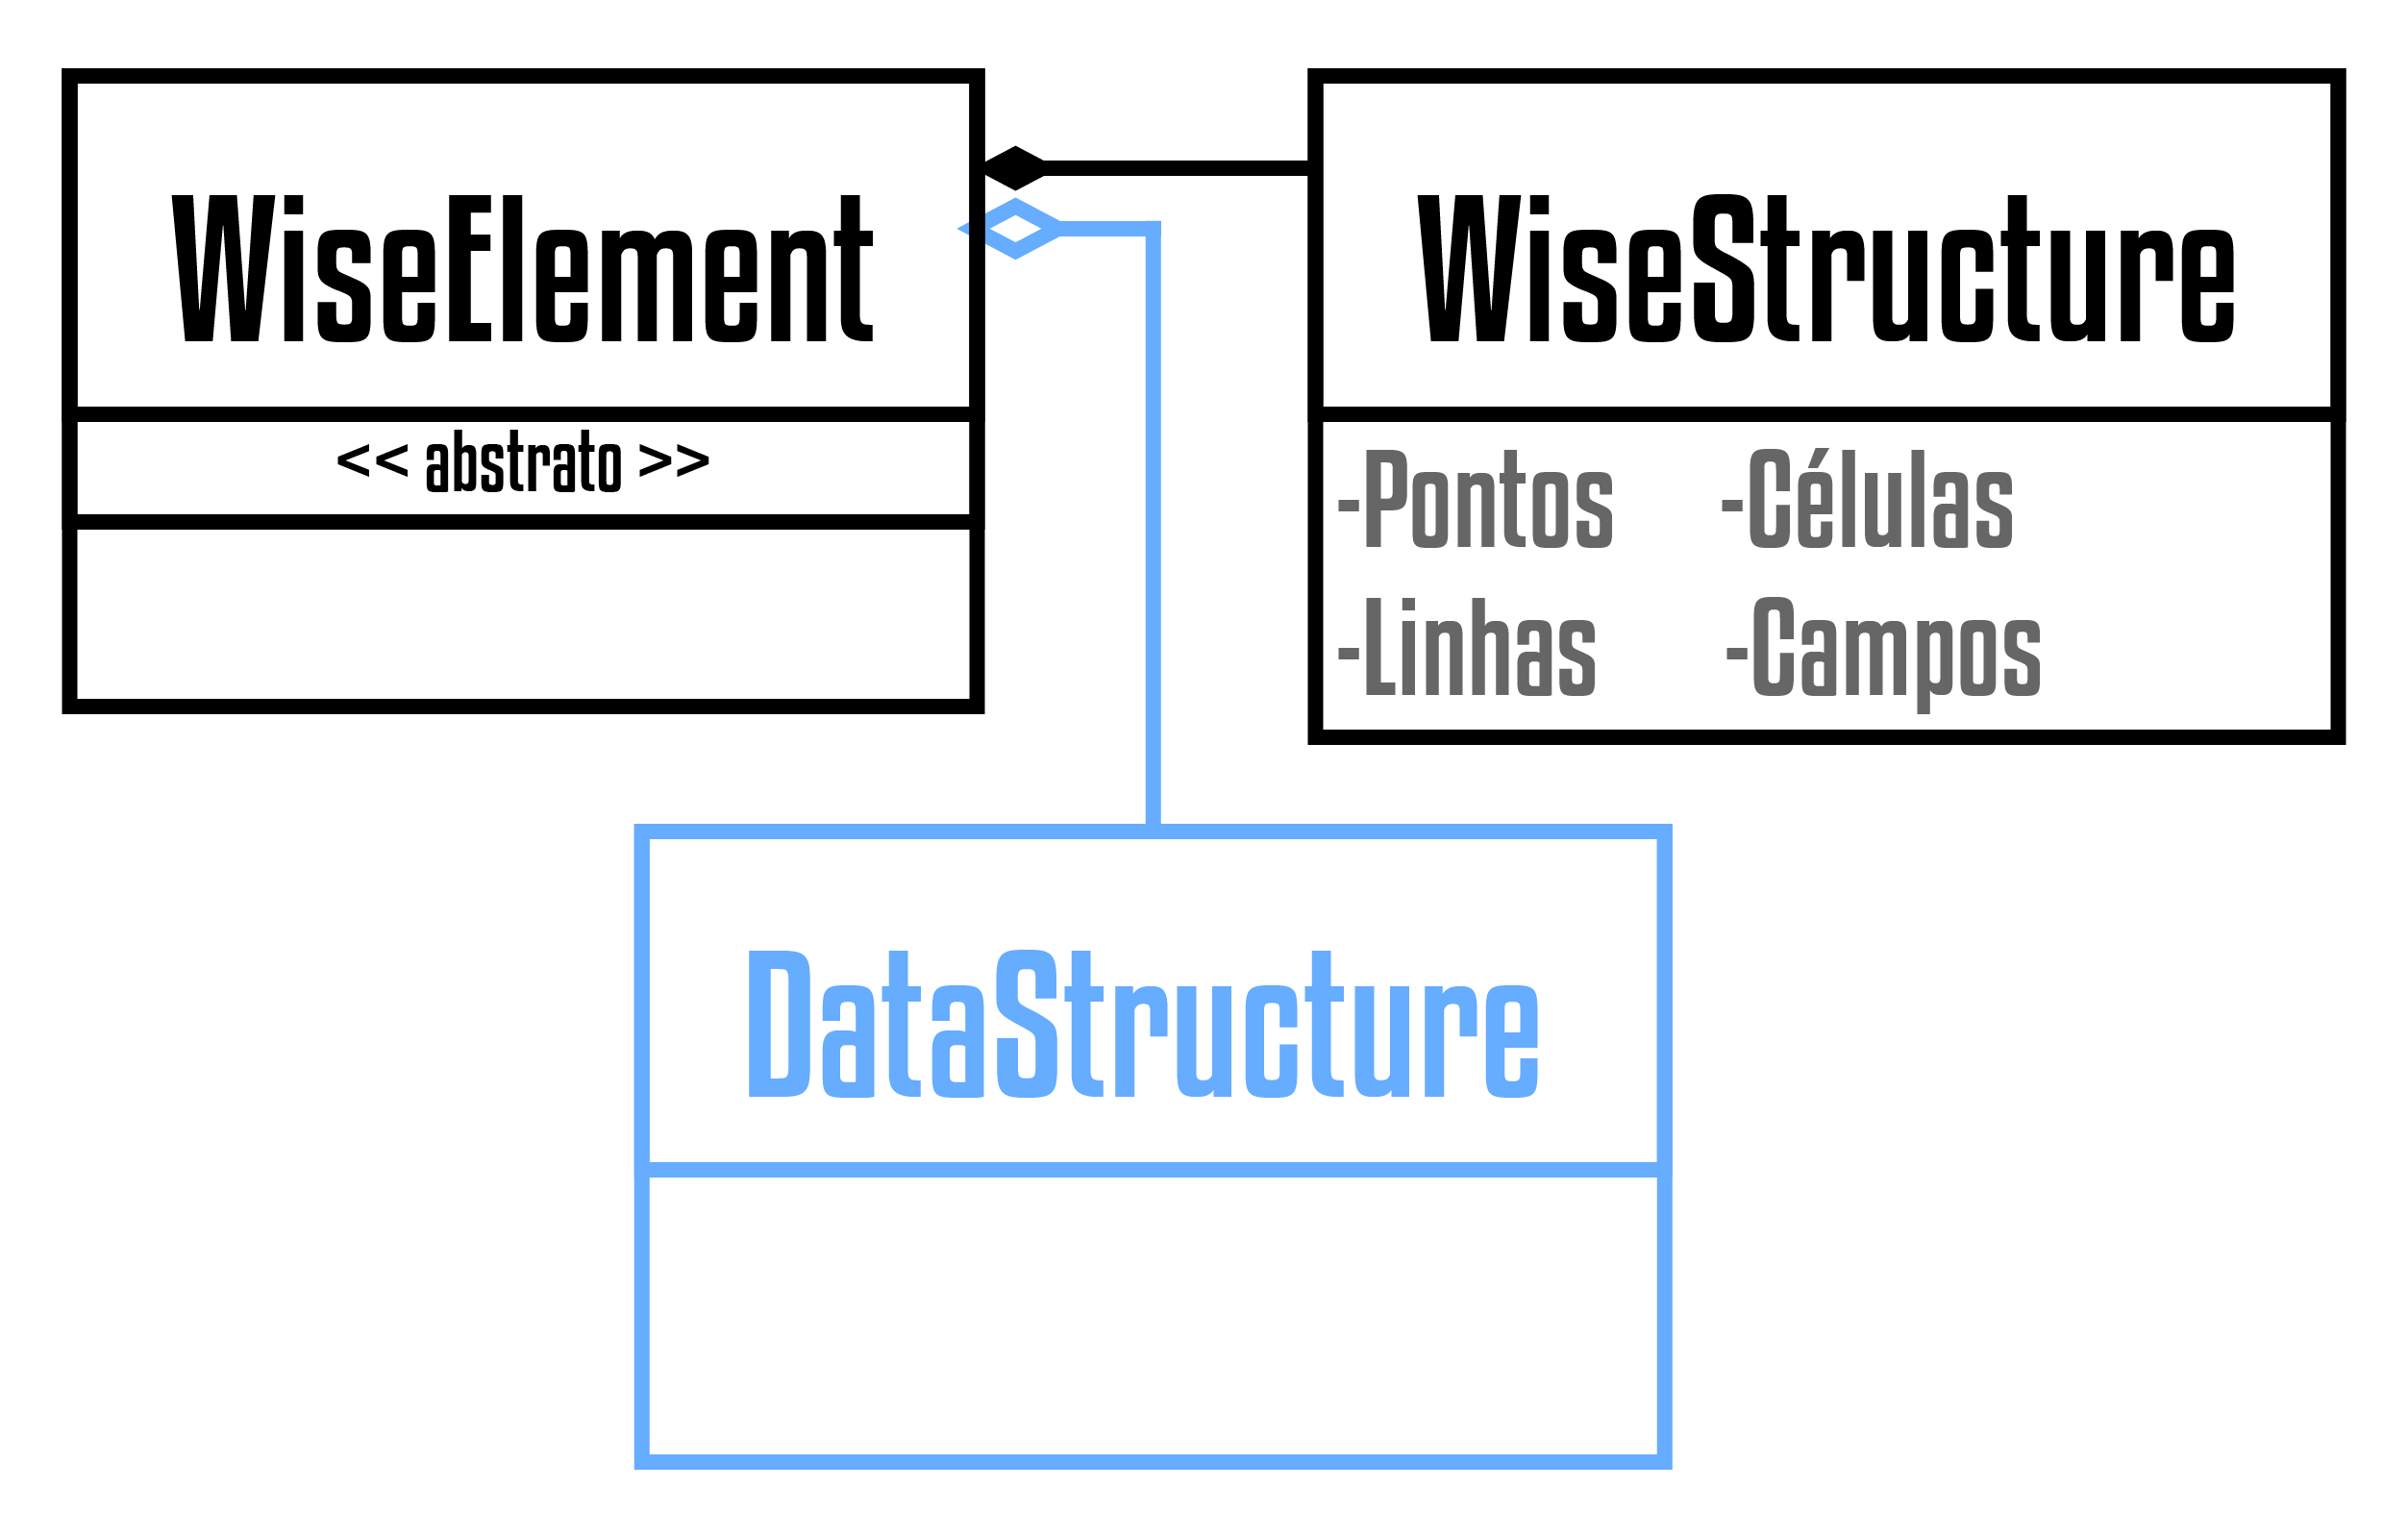
\includegraphics[width=0.45\textwidth]{Figures/WiseElement@16x.png}
			\end{multicols}
		\end{itemize}
	\end{center}
	
	\framebreak	
	
	\begin{center}
		\begin{itemize}
			\begin{multicols}{2}
				\vfill
				\item Todos os elementos inteligentes recebem a estrutura básica \textit{WiseStructure} por herança e requer por meio de funções virtuais a definição de métodos que possibilitem a manipulação dos dados abstratos.
				\columnbreak
				\item 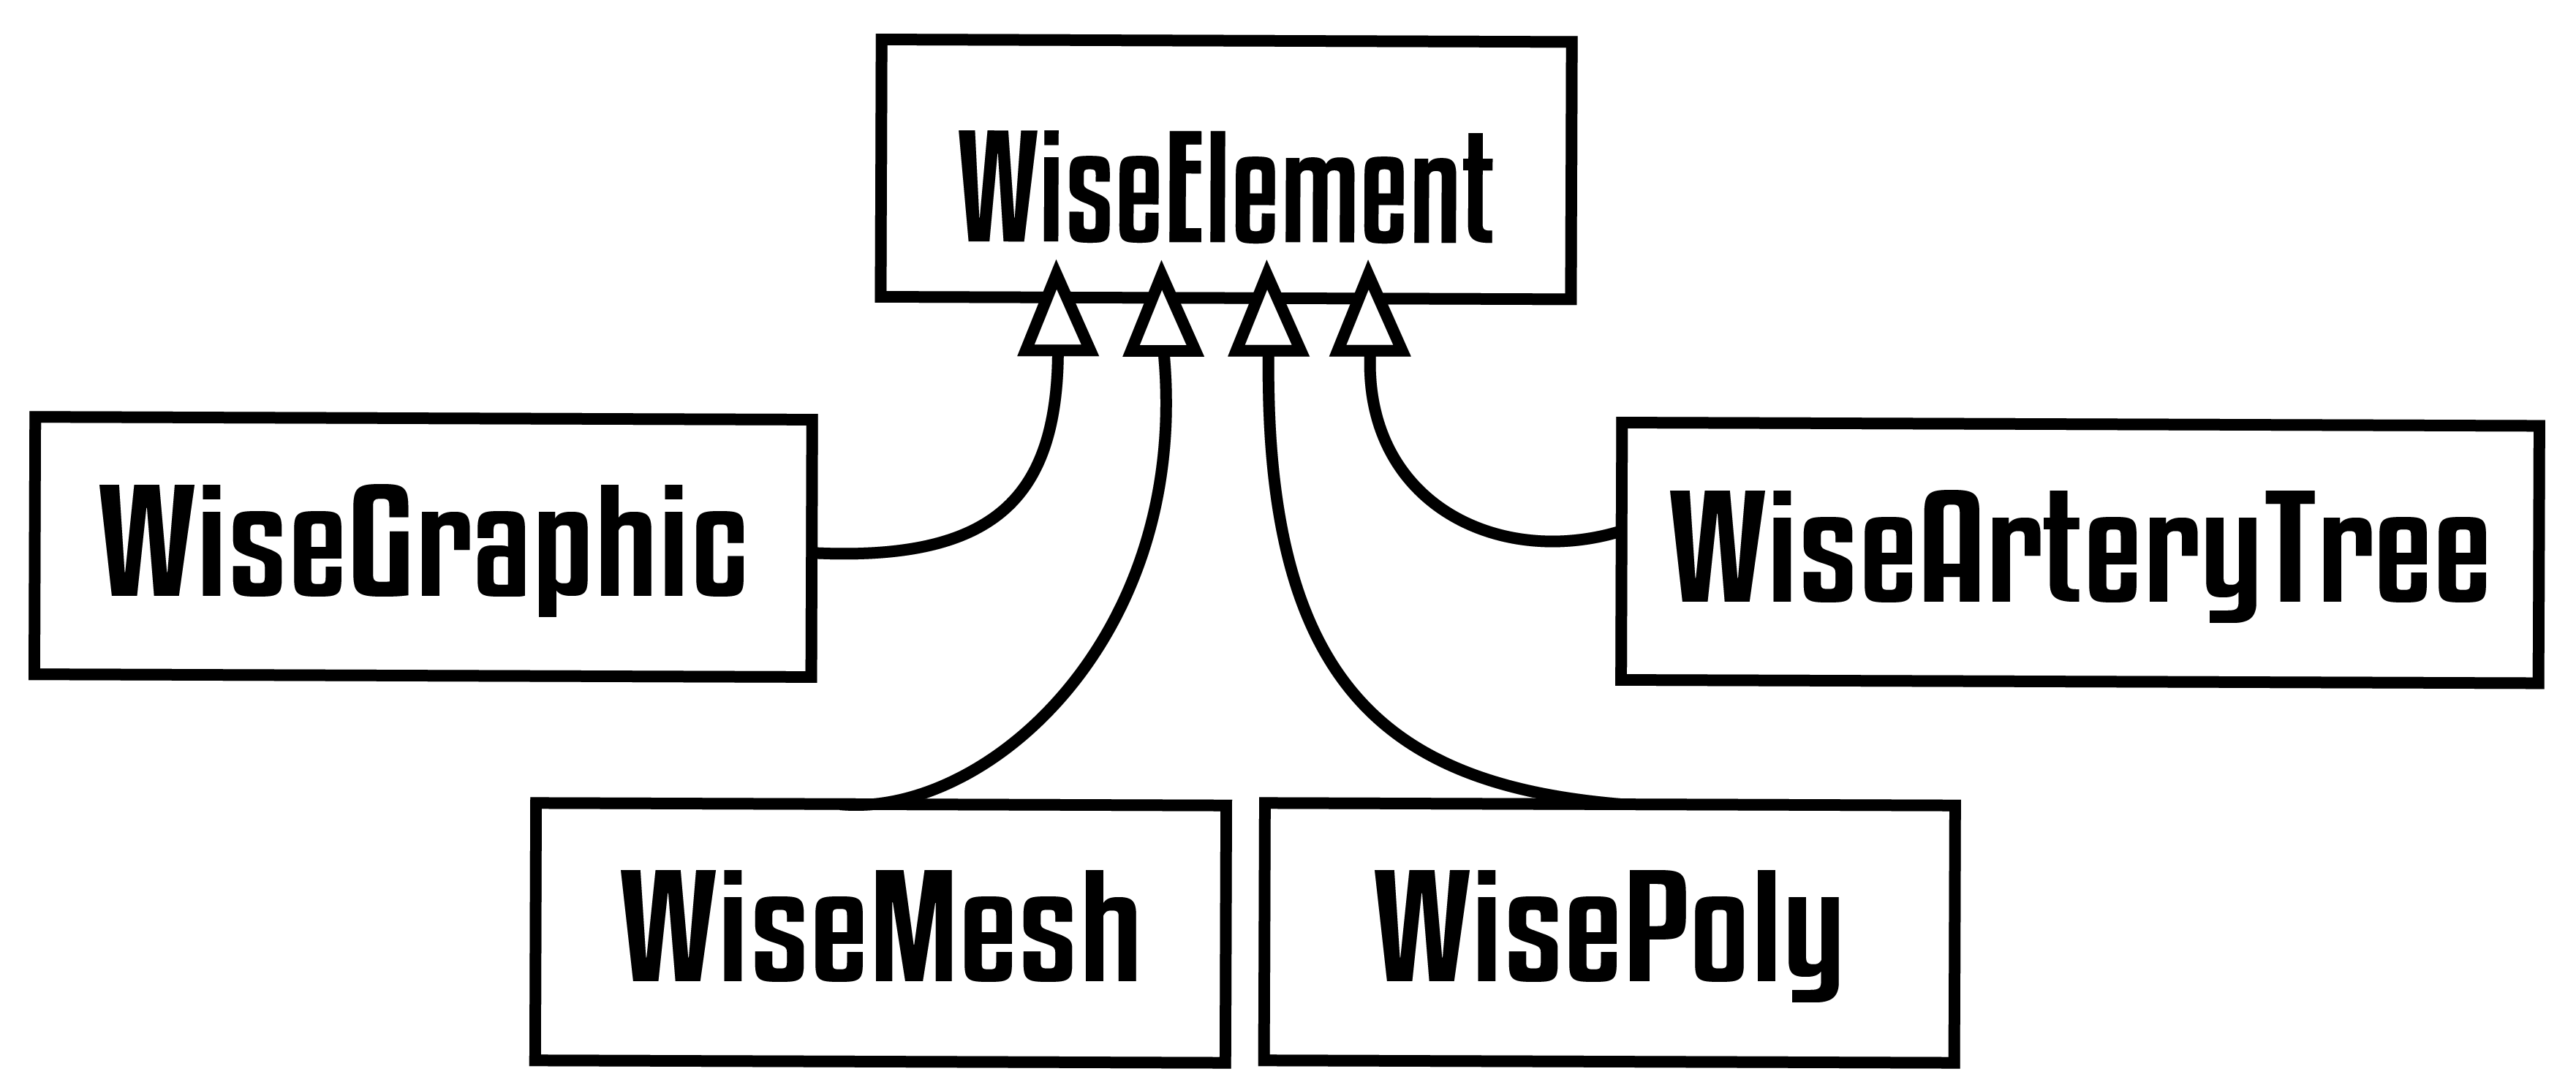
\includegraphics[width=0.45\textwidth]{Figures/WiseElements@16x.png}
			\end{multicols}
		\end{itemize}
	\end{center}
	
	\framebreak
	
	\begin{itemize}
		\item Os elementos inteligentes são regidos por uma máquina de estados, aonde os estados representam condições esperadas do elemento inteligente e as transições indicam ações tomadas com o elemento inteligente.
	\end{itemize}
	
	\framebreak
	
	\begin{center}
		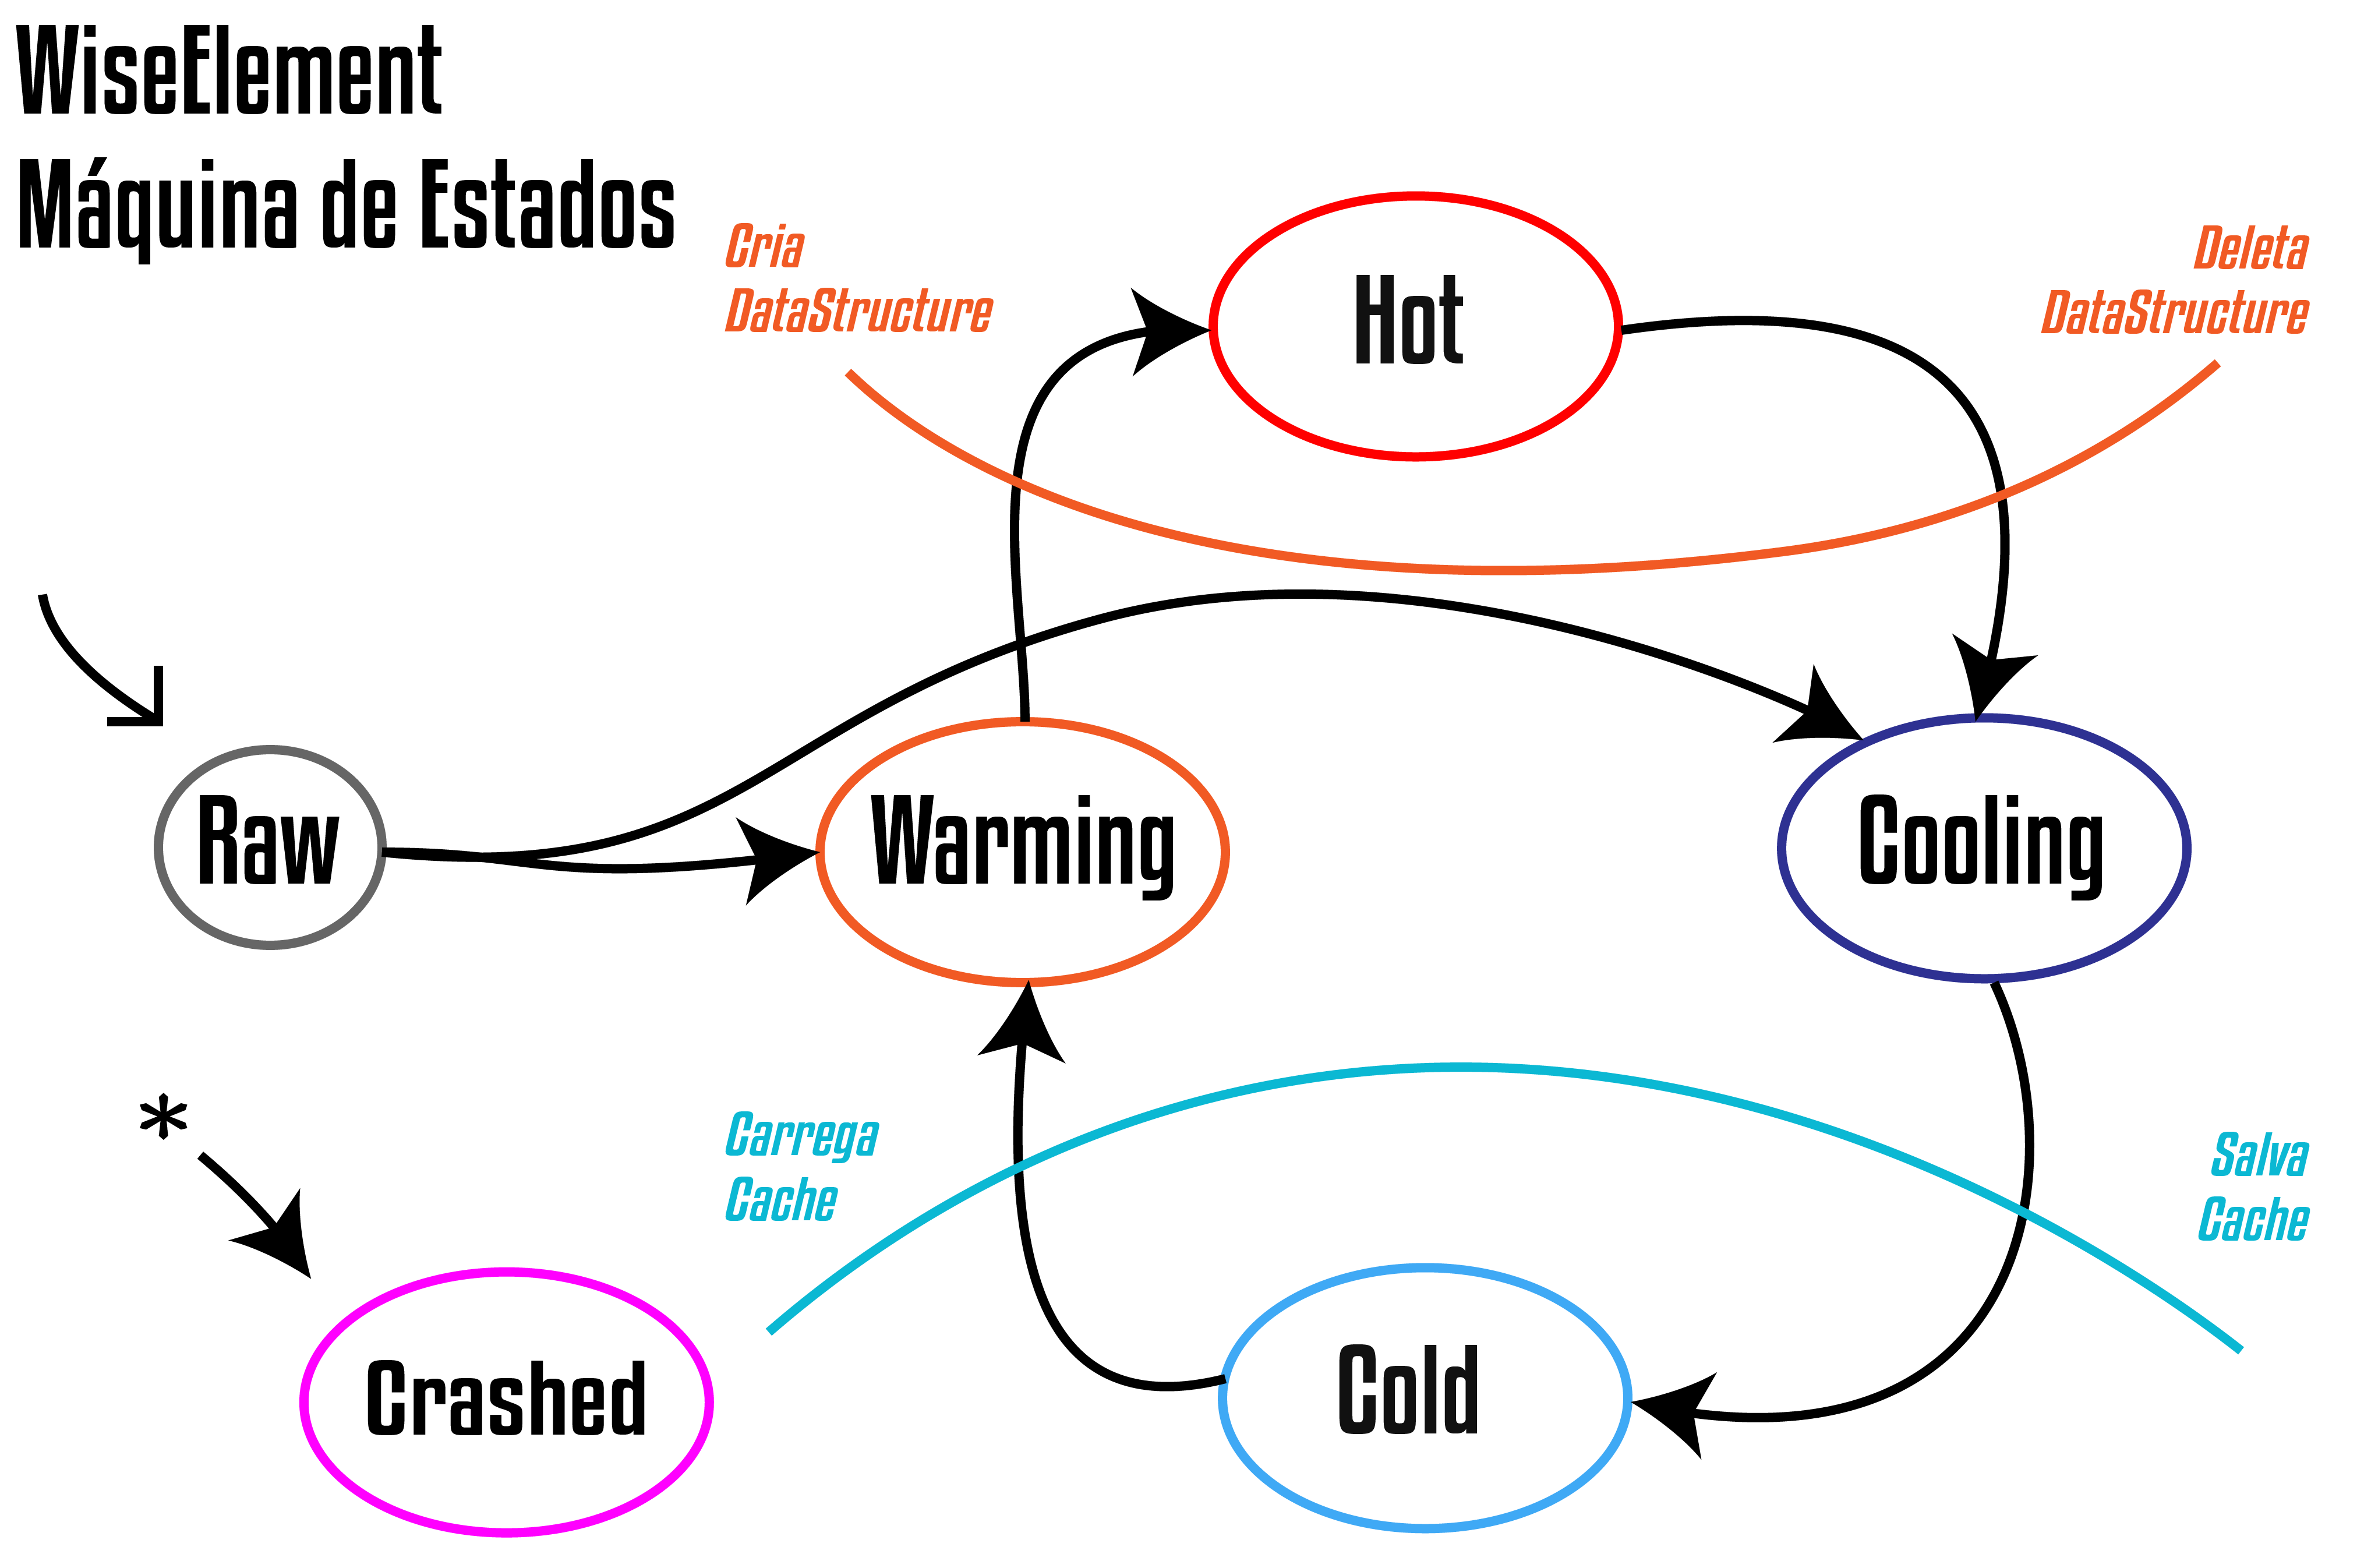
\includegraphics[width=0.6\textwidth]{Figures/WiseElementStatus@16x.png}
	\end{center}
	
	\framebreak
	
	\begin{center}
		\begin{itemize}
			\begin{multicols}{2}
				\vfill
				\item Neste estado espera-se que um elemento possua consigo ambas as estruturas presentes no elemento inteligente, seus dados abstratos e a estrutura inteligente \textit{WiseStructure}.
				\columnbreak
				\item 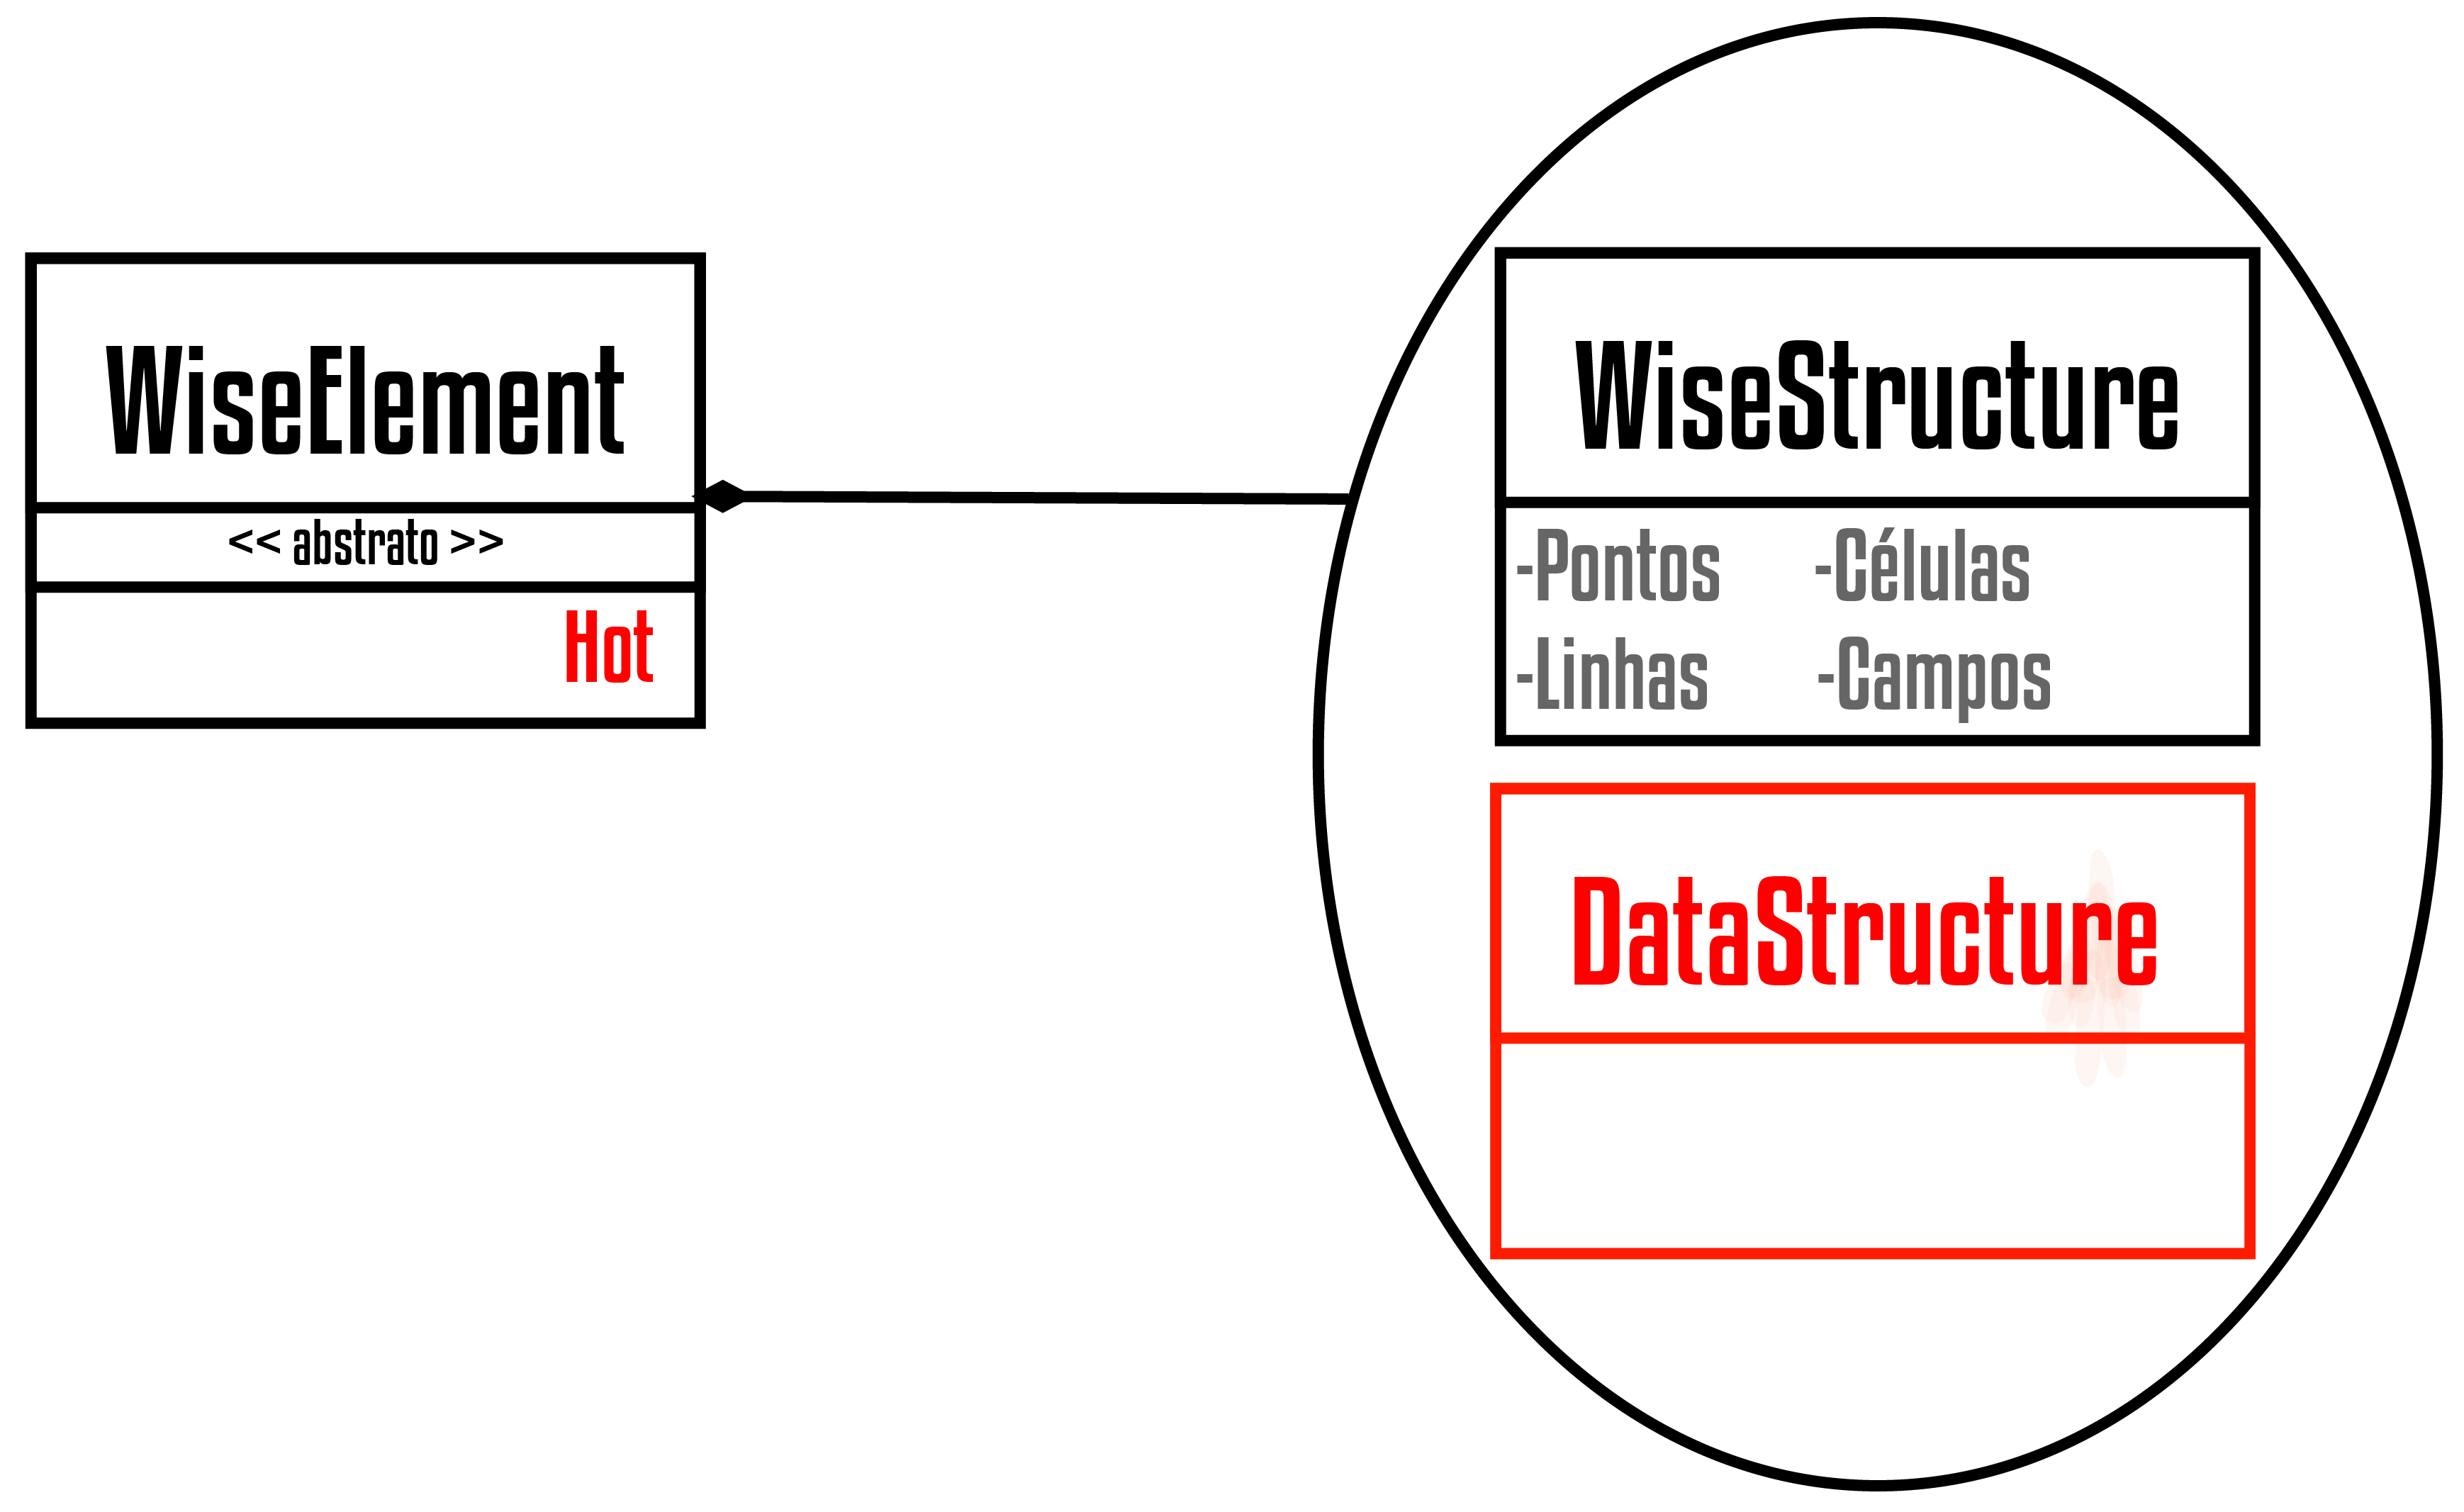
\includegraphics[width=0.45\textwidth]{Figures/WiseElementHot@16x.png}
			\end{multicols}
		\end{itemize}
	\end{center}
	
	\framebreak
	
	\begin{center}
		\begin{itemize}
			\begin{multicols}{2}
				\vfill
				\item O estado \textit{Warming} é equivalente ao estado \textit{Cooling} e \textit{Raw}.
				\item Estes estados indicam que somente a estrutura inteligente deste elemento está presente. No caso de um elemento no estado \textit{Raw}, não é esperado que a estrutura completa esteja presente nesta estrutura.
				\item Os outros estados indicam que o elemento está completamente carregado na estrutura inteligente e aguarda esfriamento ou aquecimento, processo de armazenar e recuperar arquivos em HD.
				\columnbreak
				\item 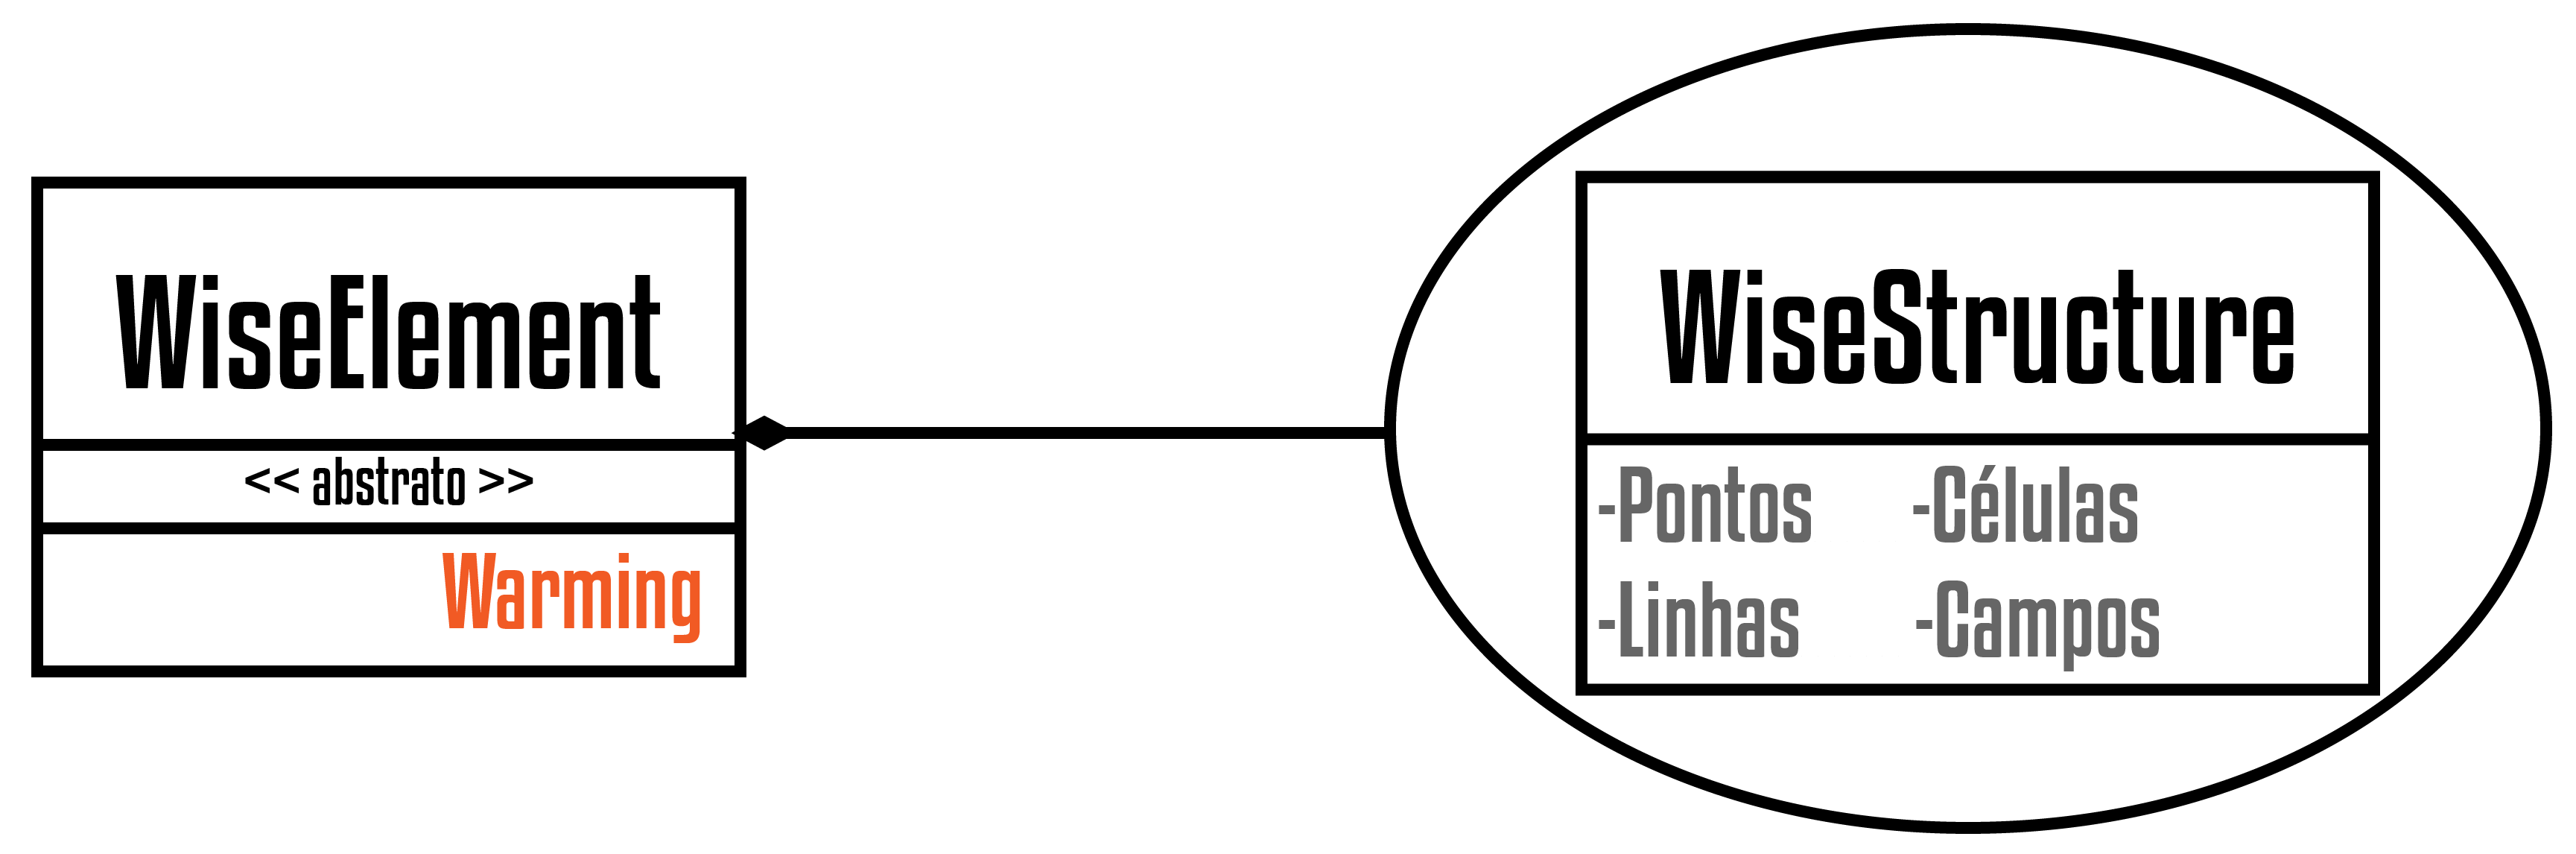
\includegraphics[width=0.45\textwidth]{Figures/WiseElementWarming@16x.png}
			\end{multicols}
		\end{itemize}
	\end{center}
	
	\framebreak
	
	\begin{center}
		\begin{itemize}
			\begin{multicols}{2}
				\vfill
				\item Espera-se que os elementos neste estado estejam salvos em HD.
				\columnbreak
				\item 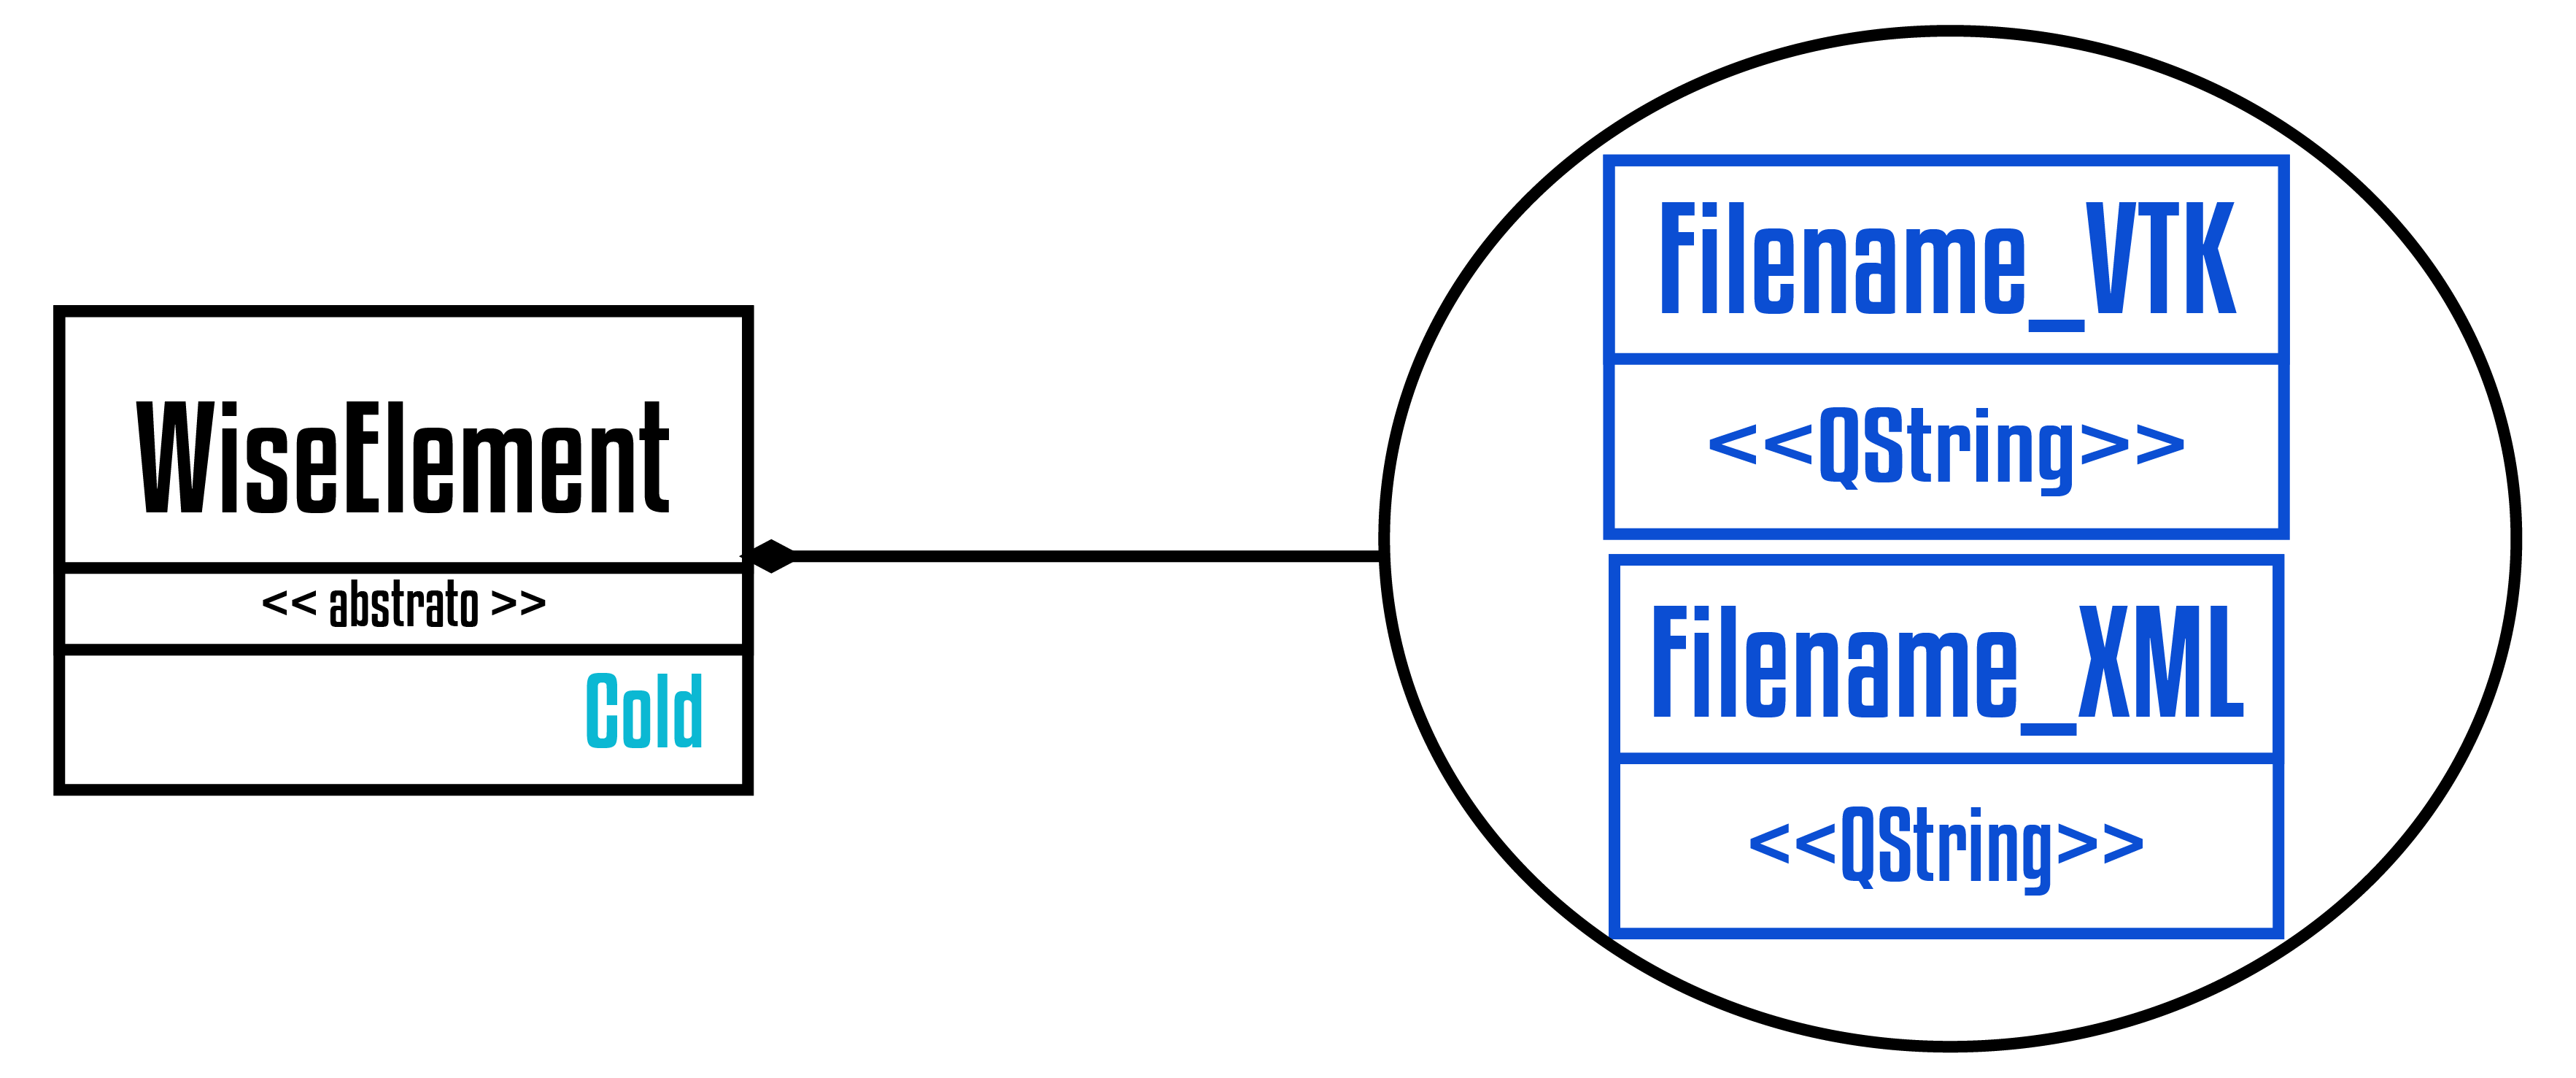
\includegraphics[width=0.45\textwidth]{Figures/WiseElementCold@16x.png}
			\end{multicols}
		\end{itemize}
	\end{center}
	
	\framebreak
	\begin{center}
		\begin{itemize}
			\begin{multicols}{2}
				\vfill
				\item Utilizando o padrão de fábricas para criar e manipular elementos inteligentes, o seguinte fluxo de trabalho foi idealizado:
				\columnbreak
				\item 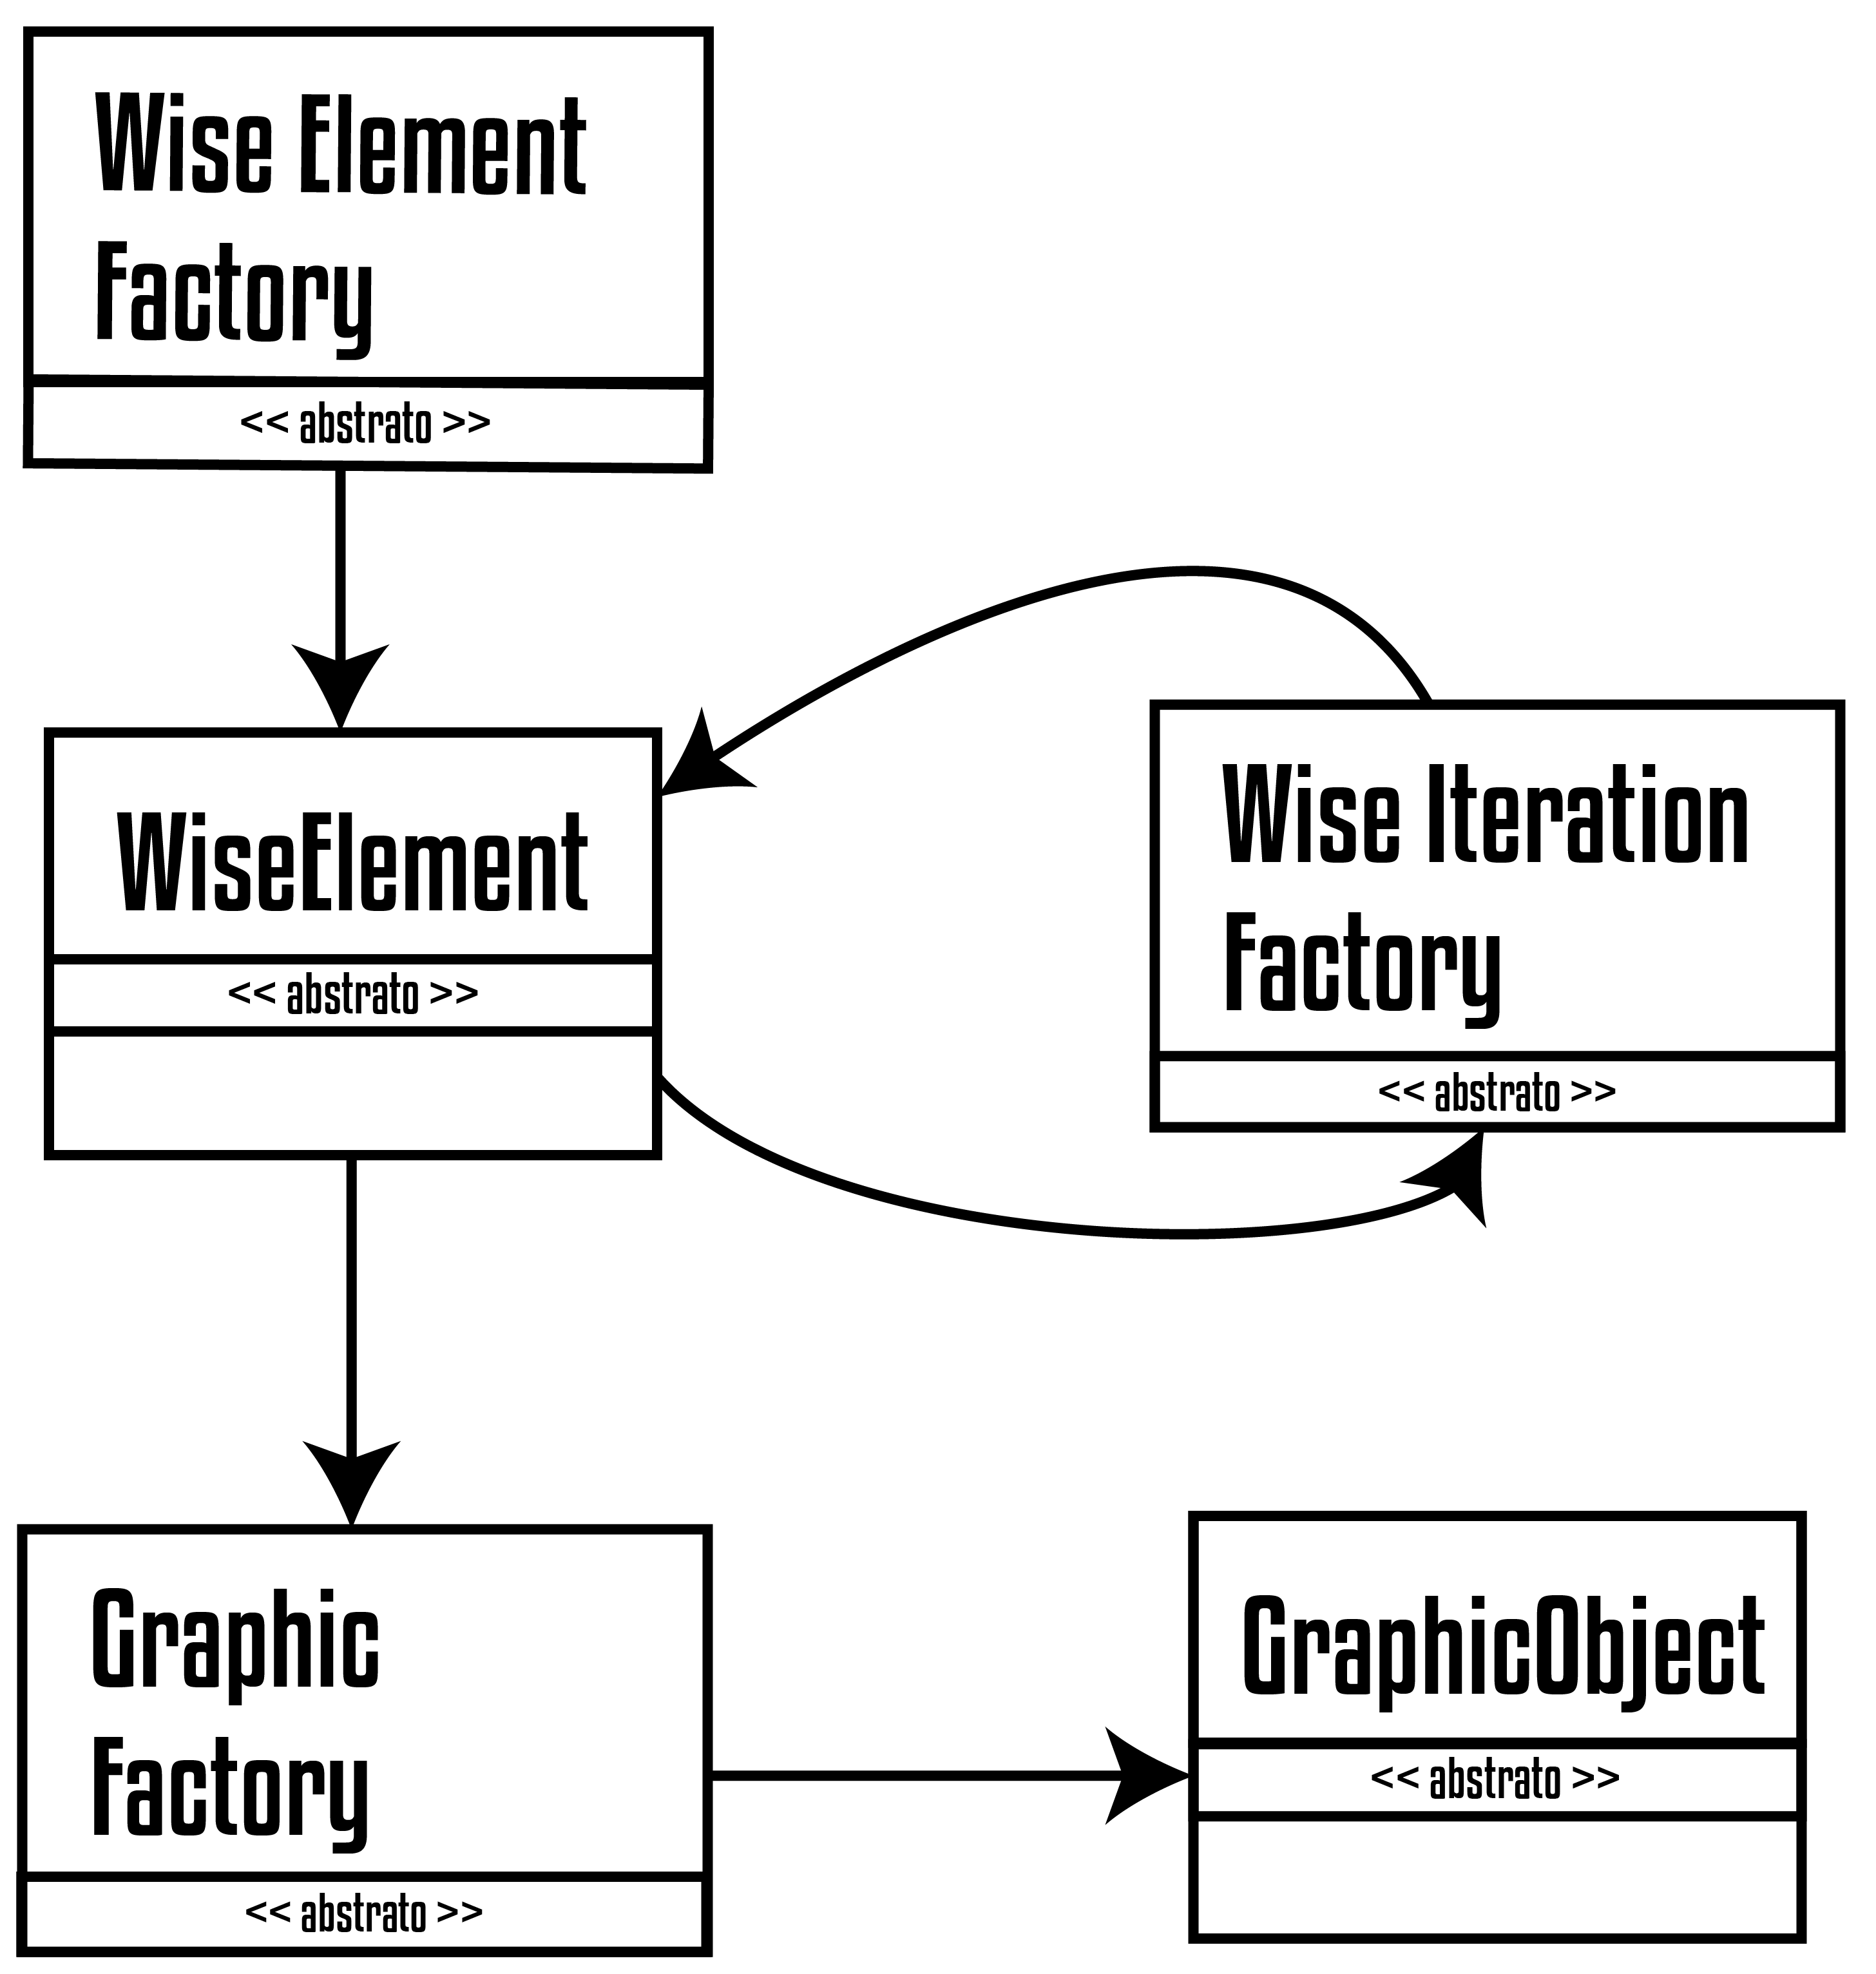
\includegraphics[width=0.45\textwidth]{Figures/WiseElementWorkflow@16x.png}
			\end{multicols}
		\end{itemize}
	\end{center}
	
	\framebreak

	\begin{itemize}
			\item A primeira fábrica \textit{WiseElementFactory} é responsável por criar corretamente cada tipo de elemento inteligente.
			\item A fábrica \textit{WiseIterationFactory} tem a função de utilizar os dados abstratos de um elemento inteligente com a finalidade de executar algum algoritmo.
			\item Finalmente, a fábrica \textit{GraphicFactory} gera os objetos capazes de se desenhar com diretivas OpenGL \textit{GraphicObject}.
	\end{itemize}	
	
	\framebreak	
	
	\framebreak
	
	\begin{itemize}
			\item O objeto inteligente \textit{WiseObject} é o objeto capaz de executar todo esse fluxo de trabalho.
	\end{itemize}	
	
	\begin{center}
		
	 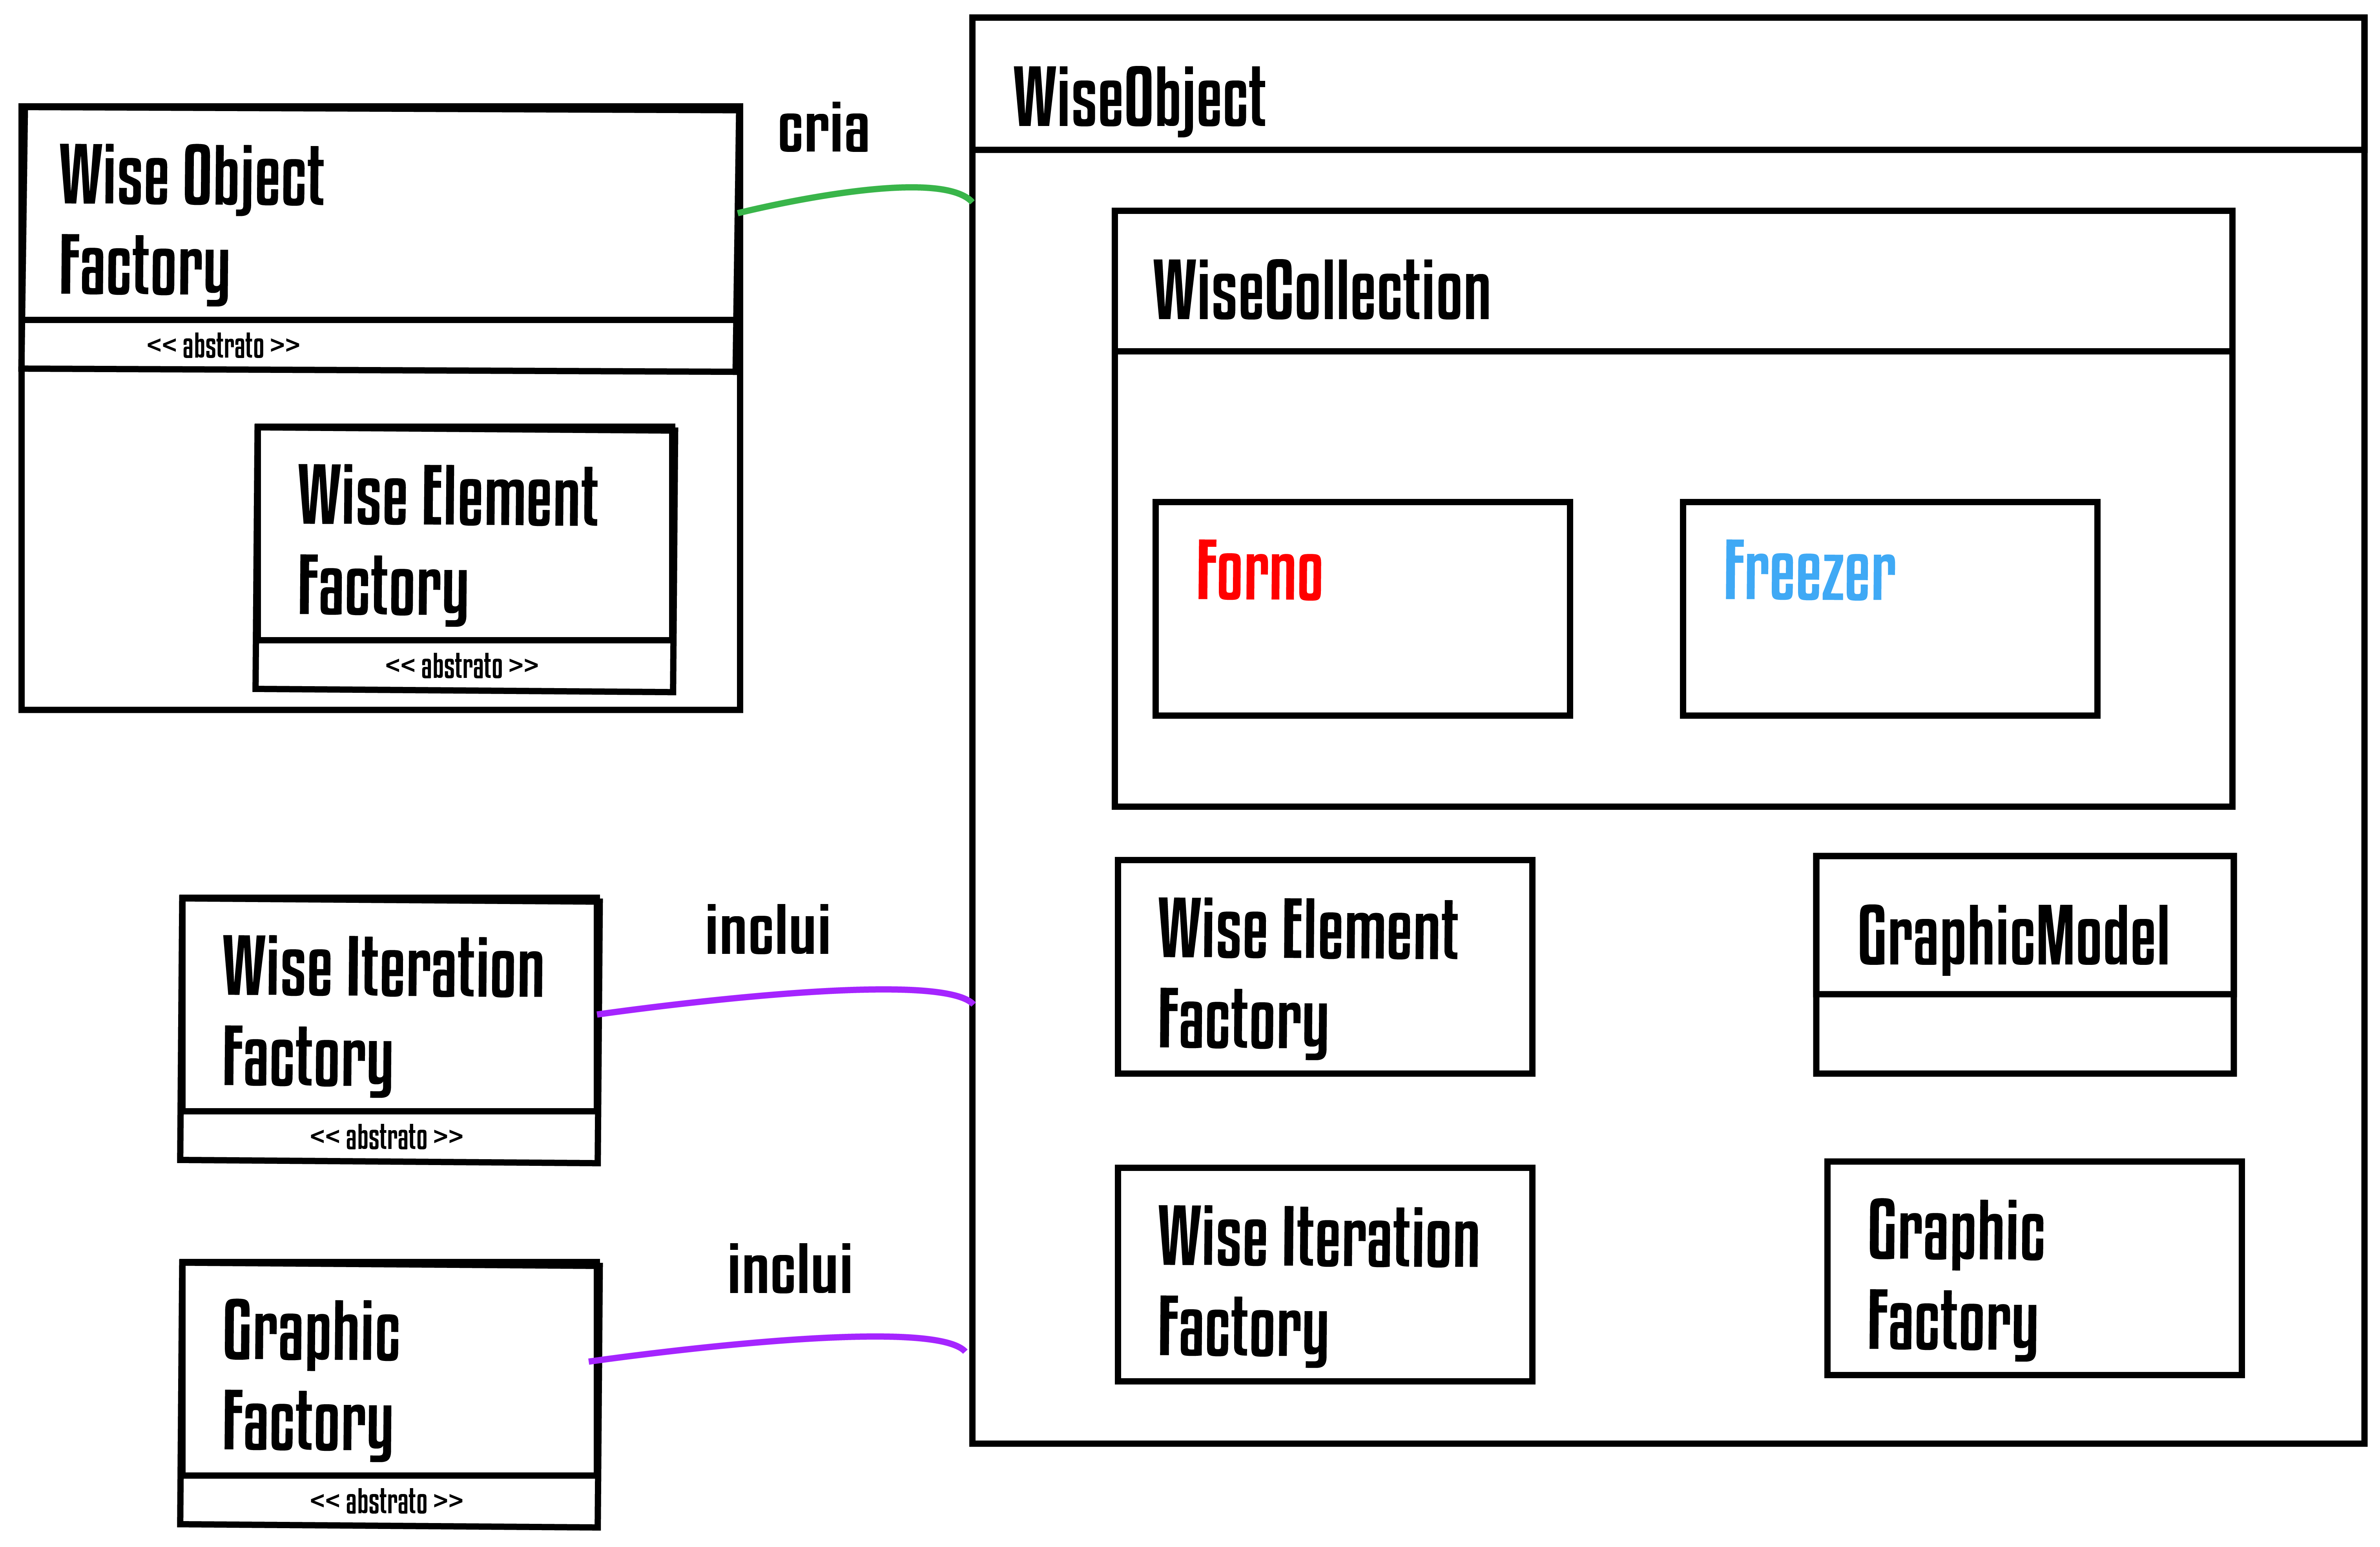
\includegraphics[width=0.7\textwidth]{Figures/WiseObject@16x.png}
		
	\end{center}
	
	\framebreak
	
	\begin{center}
		\begin{itemize}
			\begin{multicols}{2}
				\vfill
				\item Cada objeto inteligente contém uma coleção de elementos inteligentes:
				\columnbreak
				\item 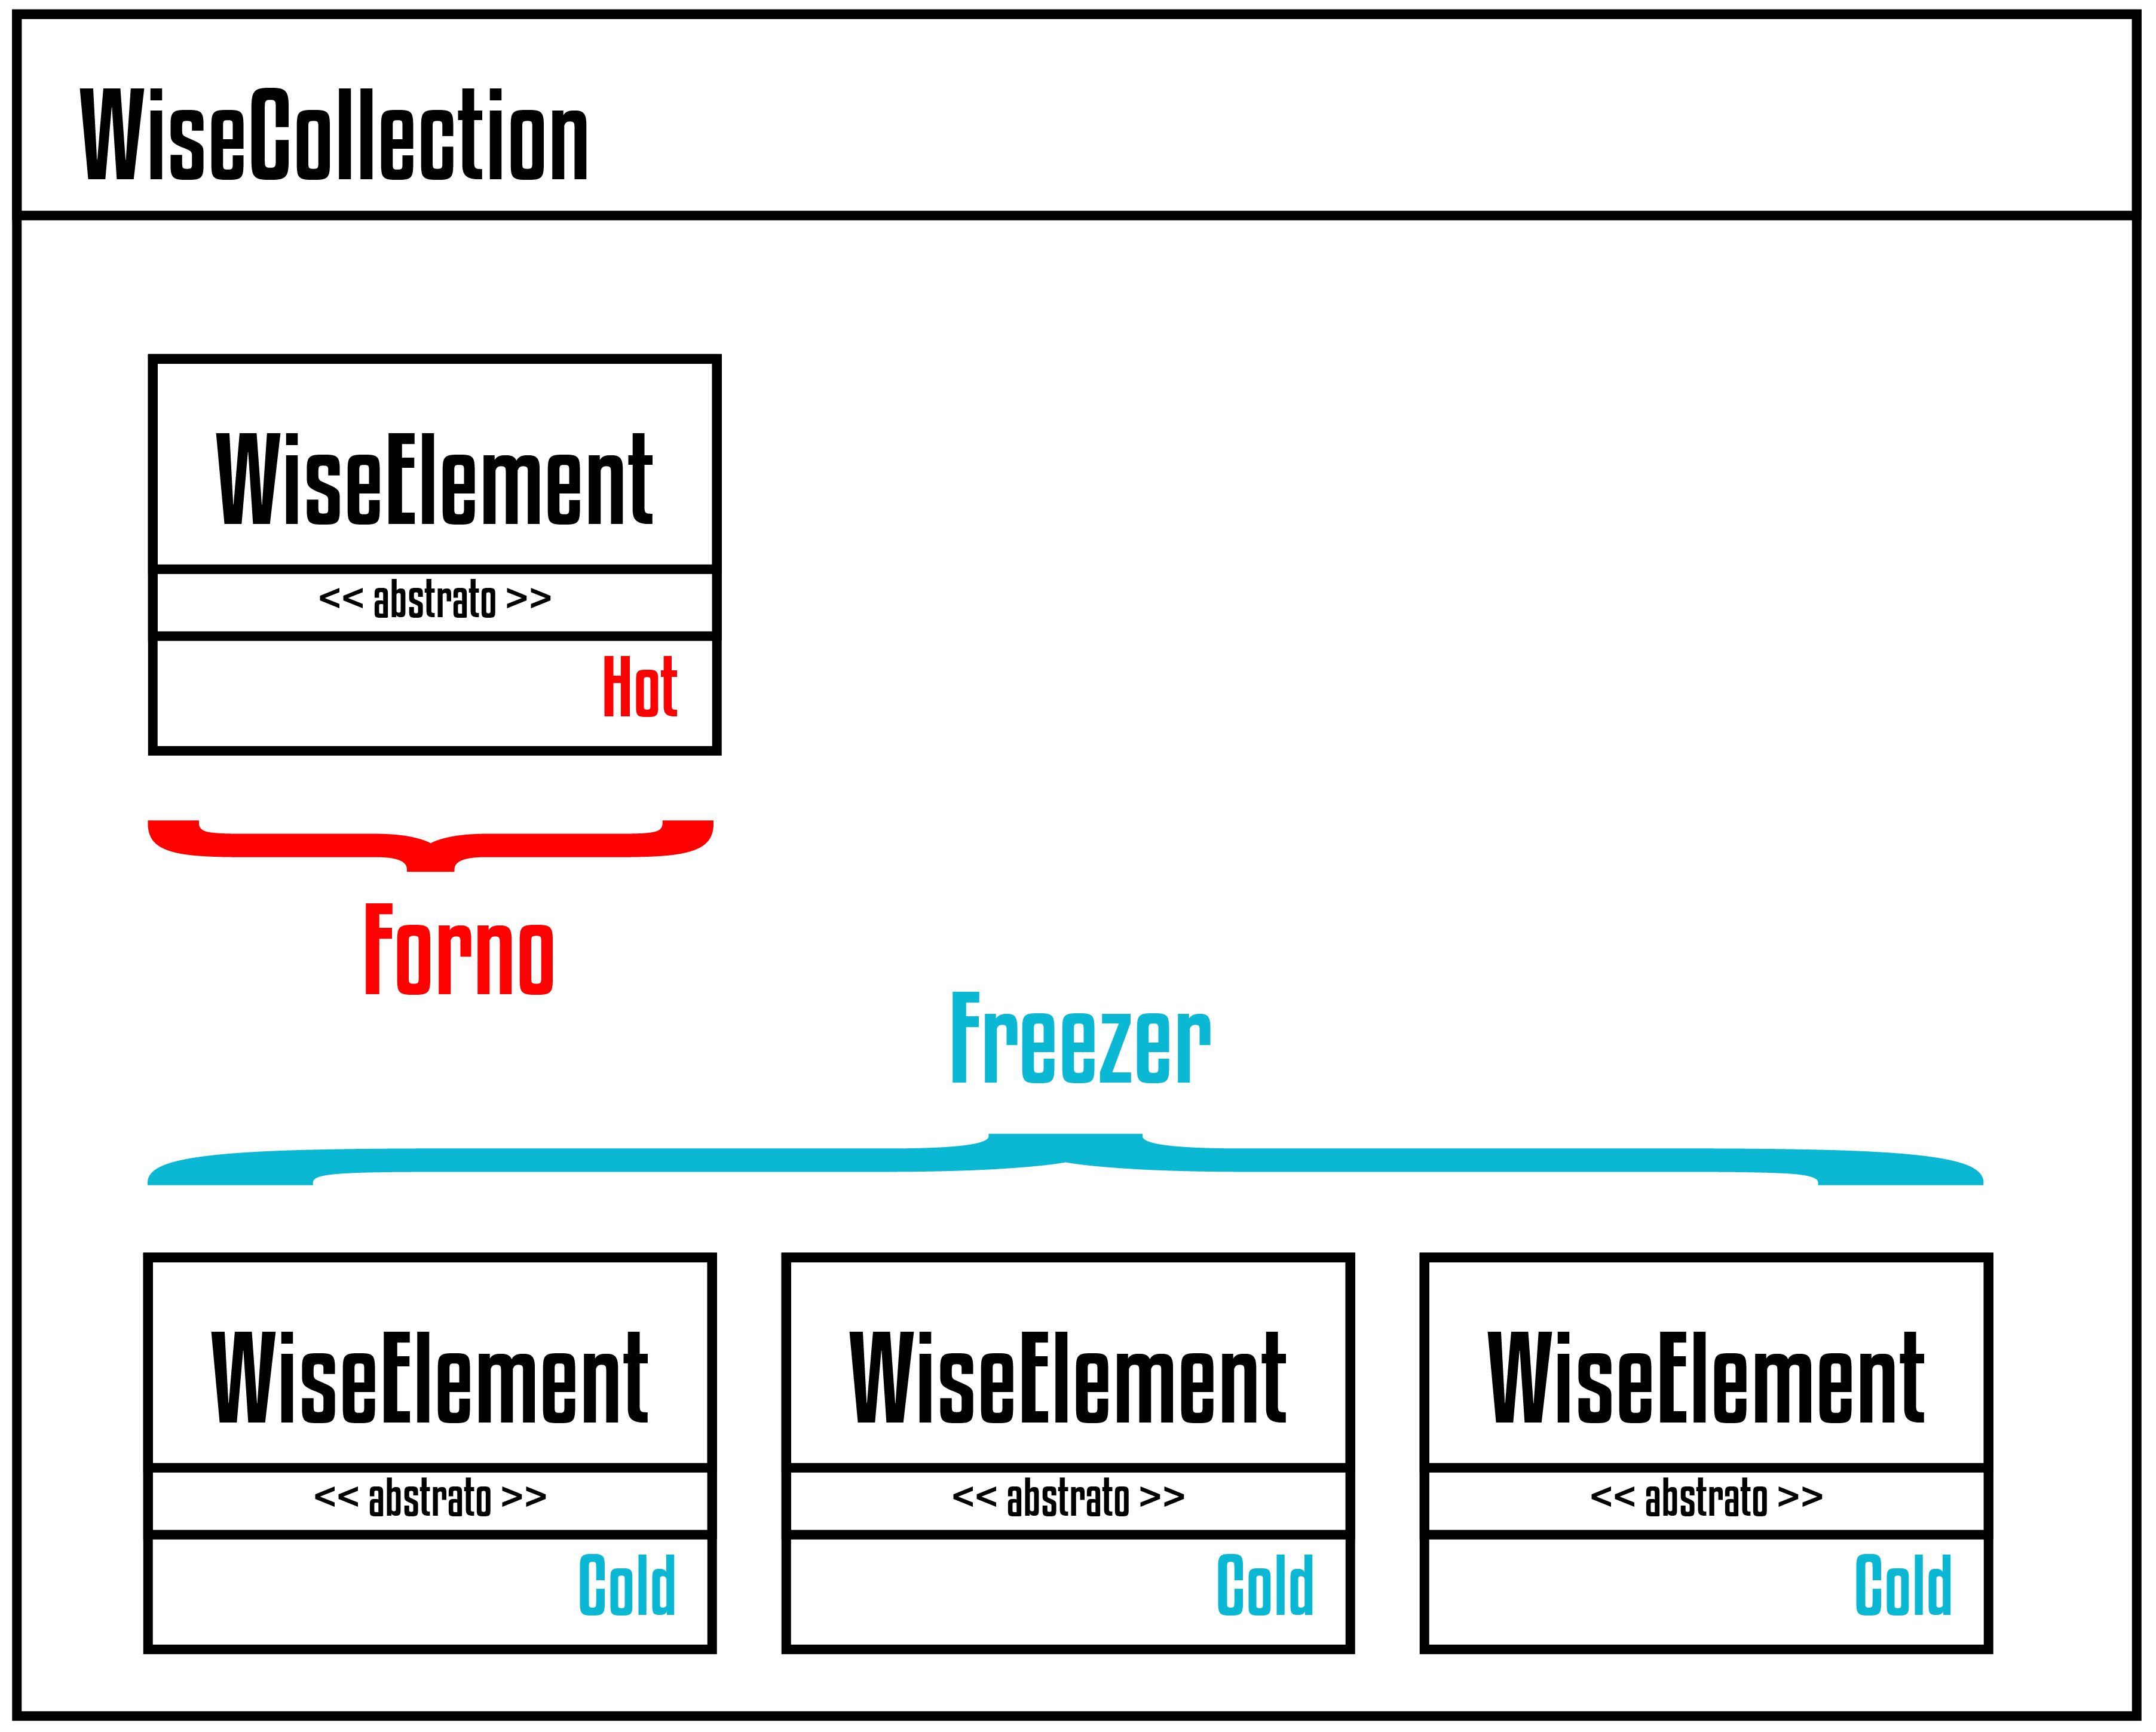
\includegraphics[width=0.45\textwidth]{Figures/WiseCollection@16x.png}
			\end{multicols}
		\end{itemize}
	\end{center}

	\framebreak
	
	\begin{itemize}
		\item Pode-se criar um objeto inteligente com um elemento inteligente, portanto é possível construir um objeto inteligente à partir de qualquer instância de elemento inteligente e sua fábrica.
		\item A estrutura \textit{Forno} é um ponteiro para um elemento que estará sempre no estado \textit{Hot}, ele representa o último elemento gerado pela iteração e é utilizado a cada nova iteração.
		\item Finalmente, a estrutura \textit{Freezer} é responsável por armazenar os elementos em cache e manter o seu registro.
	\end{itemize}
	
	\framebreak
	
	\begin{center}
		\begin{itemize}
			\begin{multicols}{2}
				\vfill
				\item É possível também que seja incluída a estrutura de visualização do objeto inteligente:
				\columnbreak
				\item 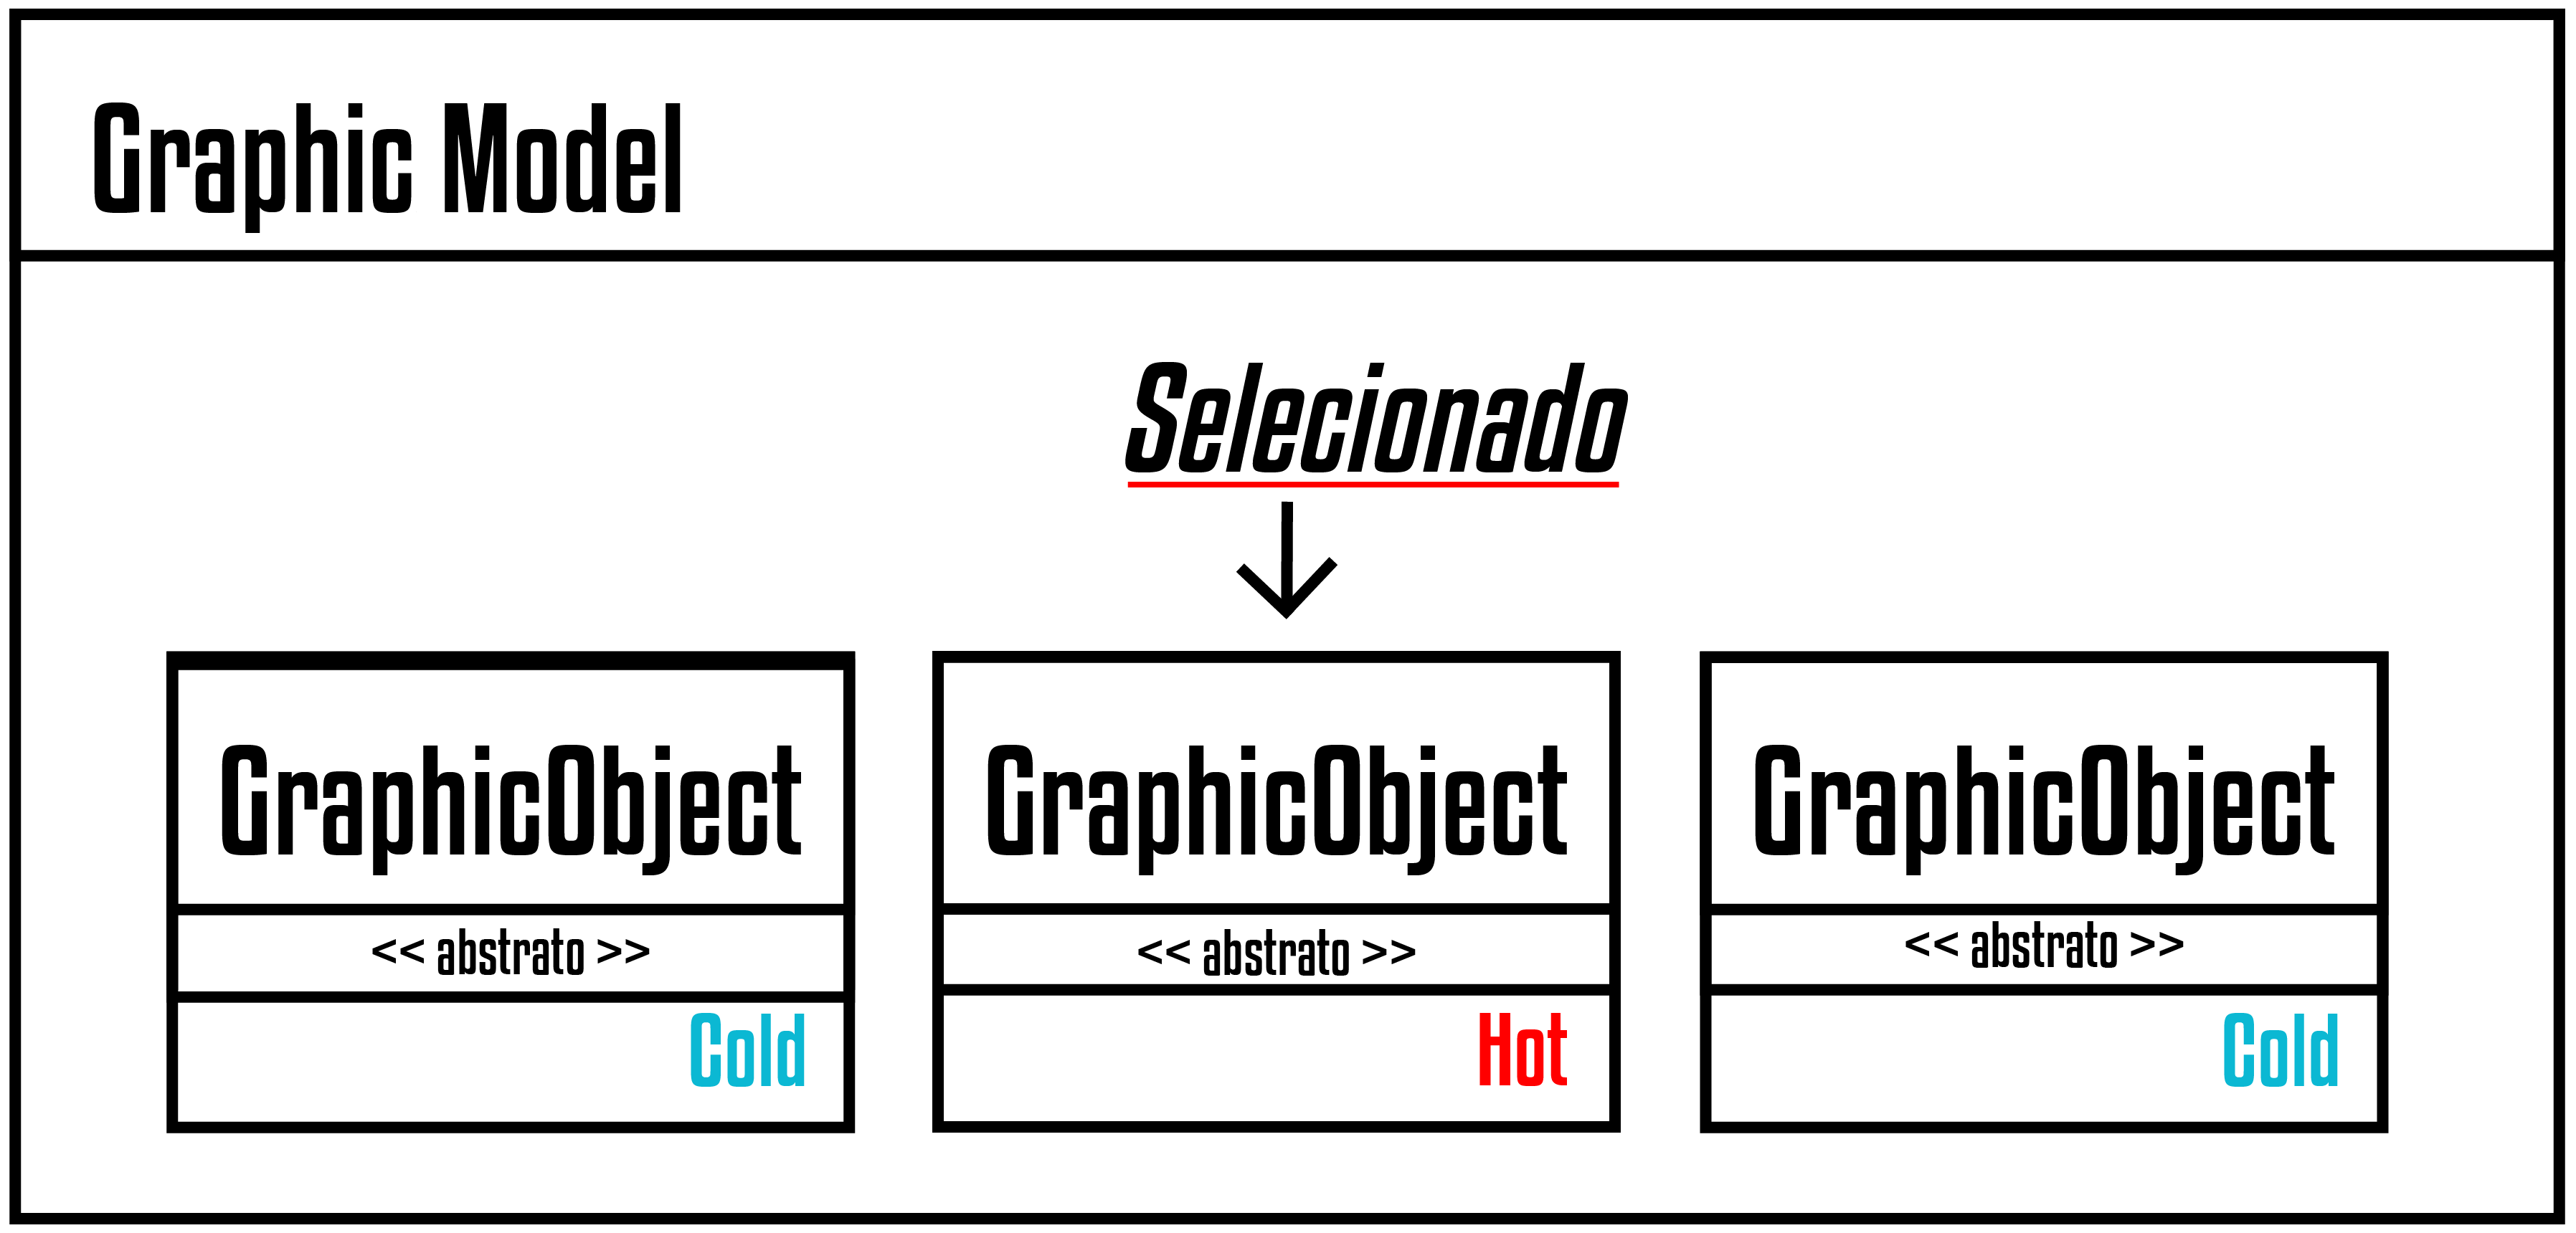
\includegraphics[width=0.45\textwidth]{Figures/GraphicModel@16x.png}
			\end{multicols}
		\end{itemize}
	\end{center}

	\framebreak
	
	\begin{center}
		\begin{itemize}
			\begin{multicols}{2}
				\vfill
				\item Os objetos gráficos são objetos que possuem uma lista de elementos gráficos com valores e é capas de desenhá-los em um quadro OpenGL.
				\item O modelo gráfico \textit{GraphicModel} irá manter a coleção de objetos gráficos em memória conforme a necessidade para visualização, mantendo uma quantidade mínima de objetos em memória a todo momento.
				\columnbreak
				\item 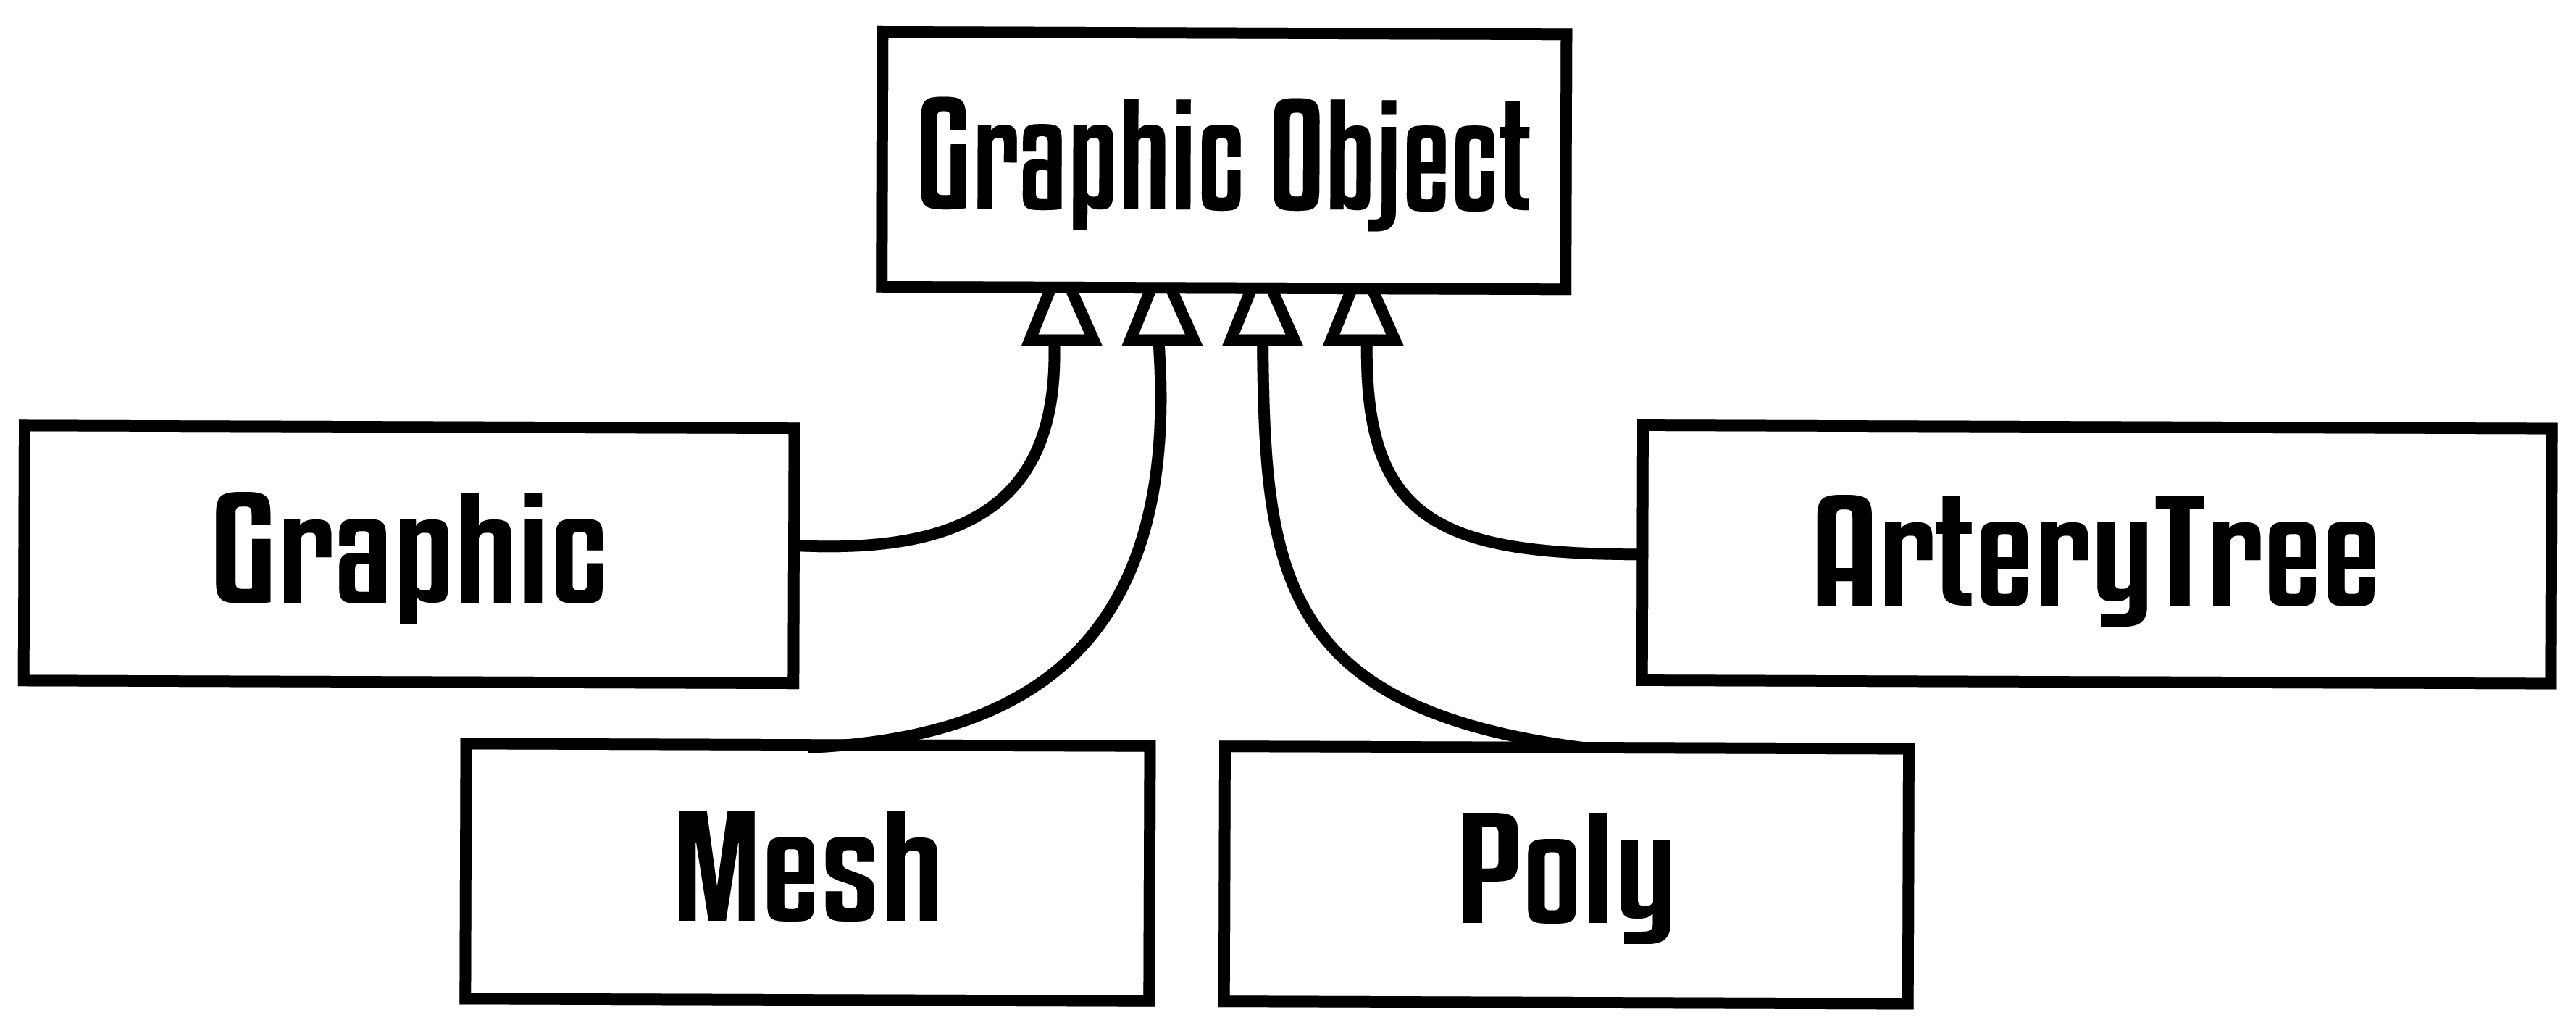
\includegraphics[width=0.45\textwidth]{Figures/GraphicObjects@16x.png}
			\end{multicols}
		\end{itemize}
	\end{center}
	
	\framebreak
	
	\begin{center}
		\begin{itemize}
			\begin{multicols}{2}
				\vfill
				\item Objetos gráficos também possuem uma máquina de estados que dita se a estrutura está presente em memória ou armazenada em cache:
				\columnbreak
				\item 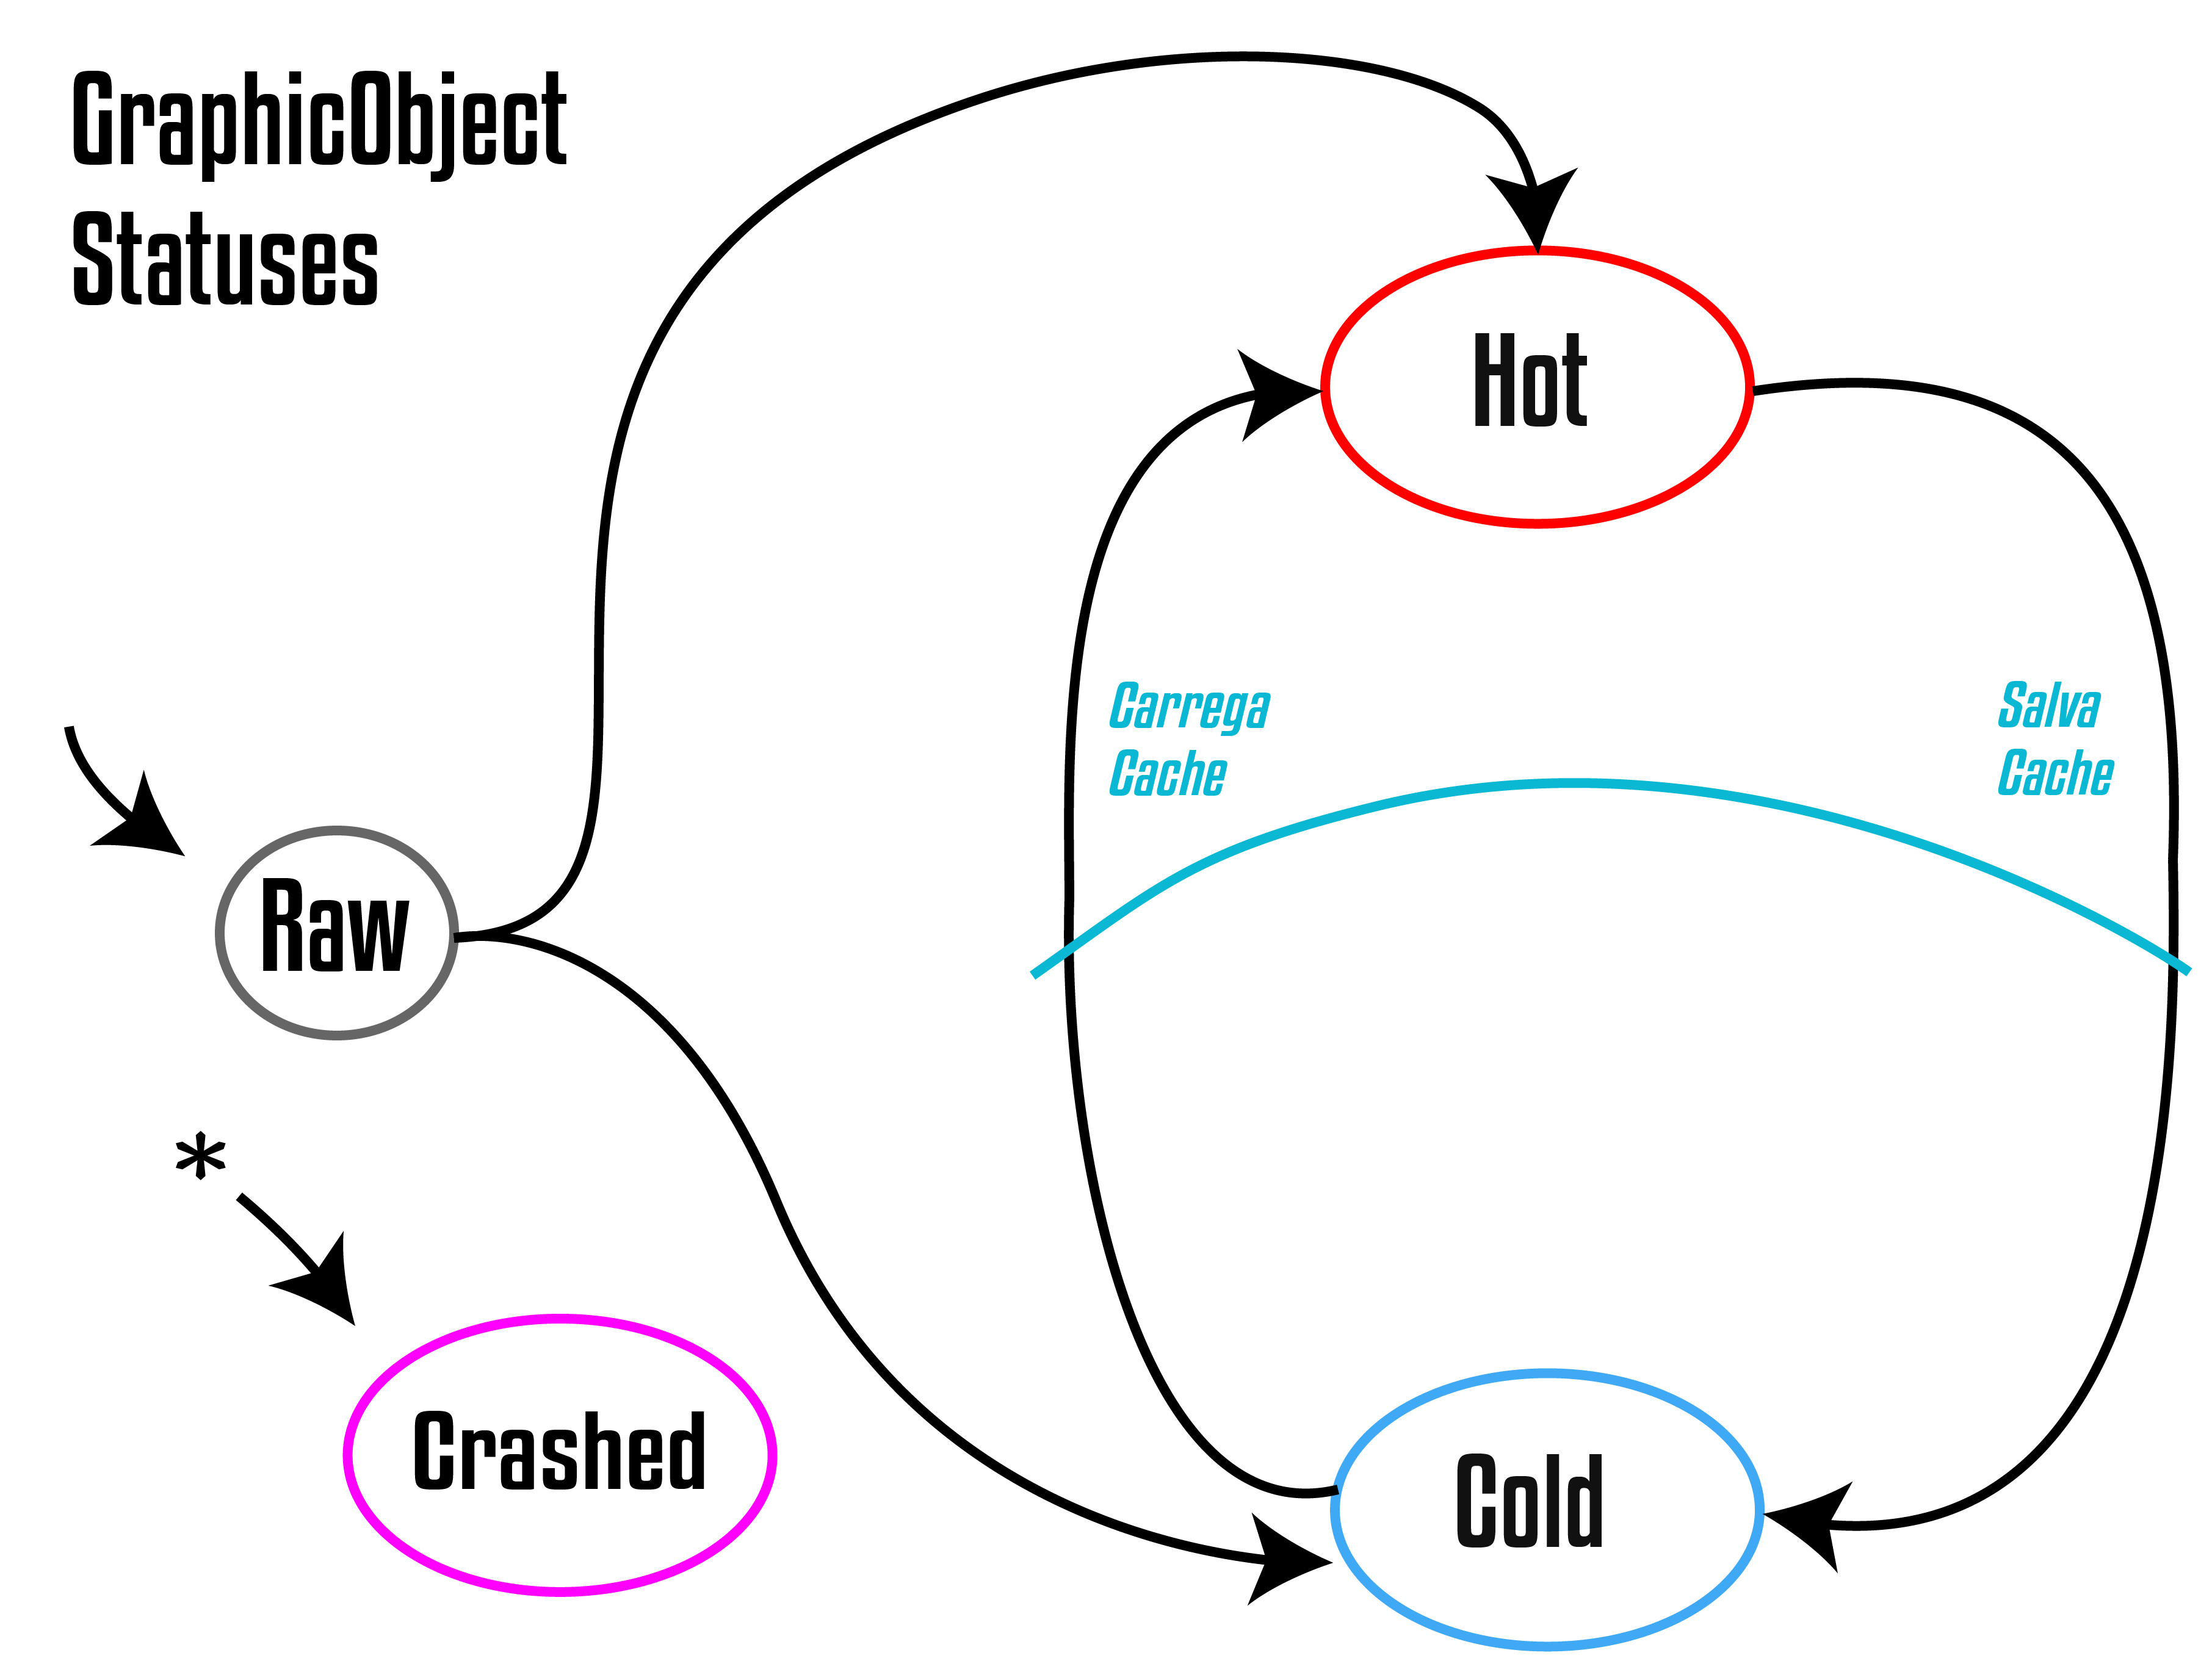
\includegraphics[width=0.45\textwidth]{Figures/GraphicObjectStatus@16x.png}
			\end{multicols}
		\end{itemize}
	\end{center}
	
	\framebreak
	\begin{itemize}
			\item Os elementos gráficos são todas as instâncias que implementam a classe abstrata \textit{GraphicElement}:
	\end{itemize}		
	
	\begin{center}
		
		\item 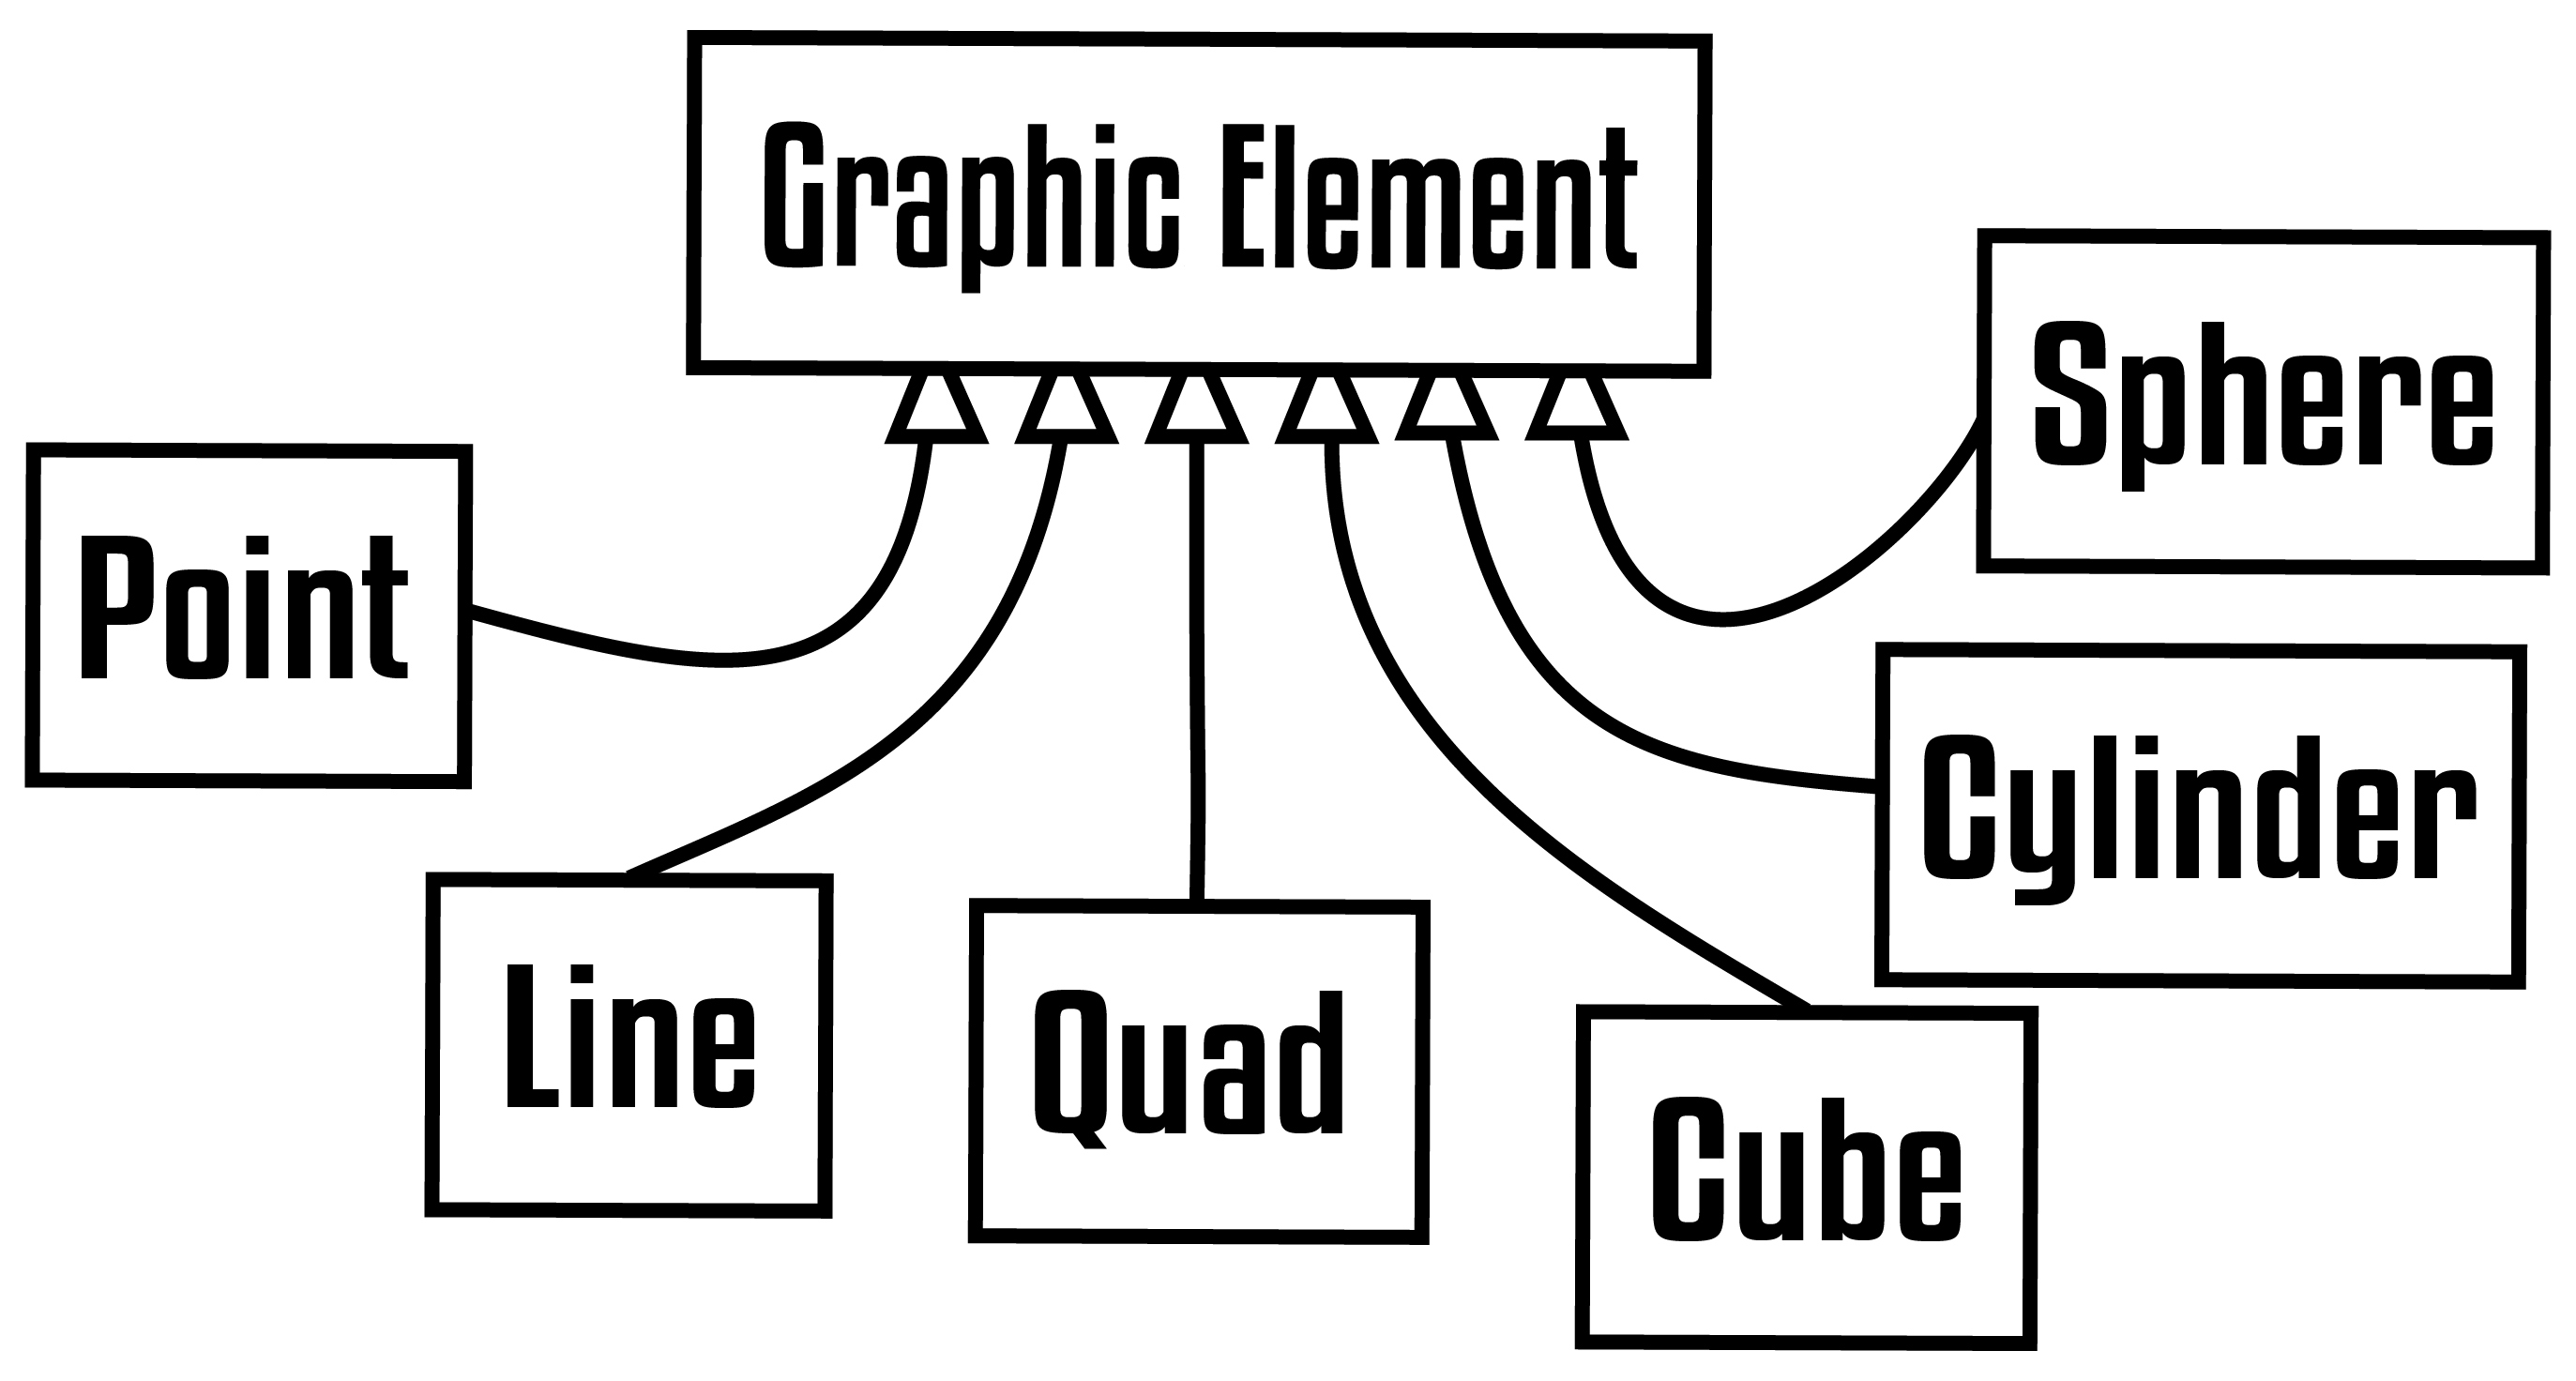
\includegraphics[width=0.6\textwidth]{Figures/GraphicElements@16x.png}
		
	\end{center}
	
	\begin{itemize}
		\item Os elementos gráficos armazenam os pontos necessários para desenhá-lo e um valor associado. Este valor associado corresponde à algum valor armazenado em um ponto, uma linha, uma célula ou um campo da \textit{WiseStructure}.
	\end{itemize}
	
	\framebreak

	\begin{itemize}
			\item Os objetos inteligentes \textit{WiseObject} possuem também uma máquina de estados:
	\end{itemize}		
	
	\begin{center}
		
		\item 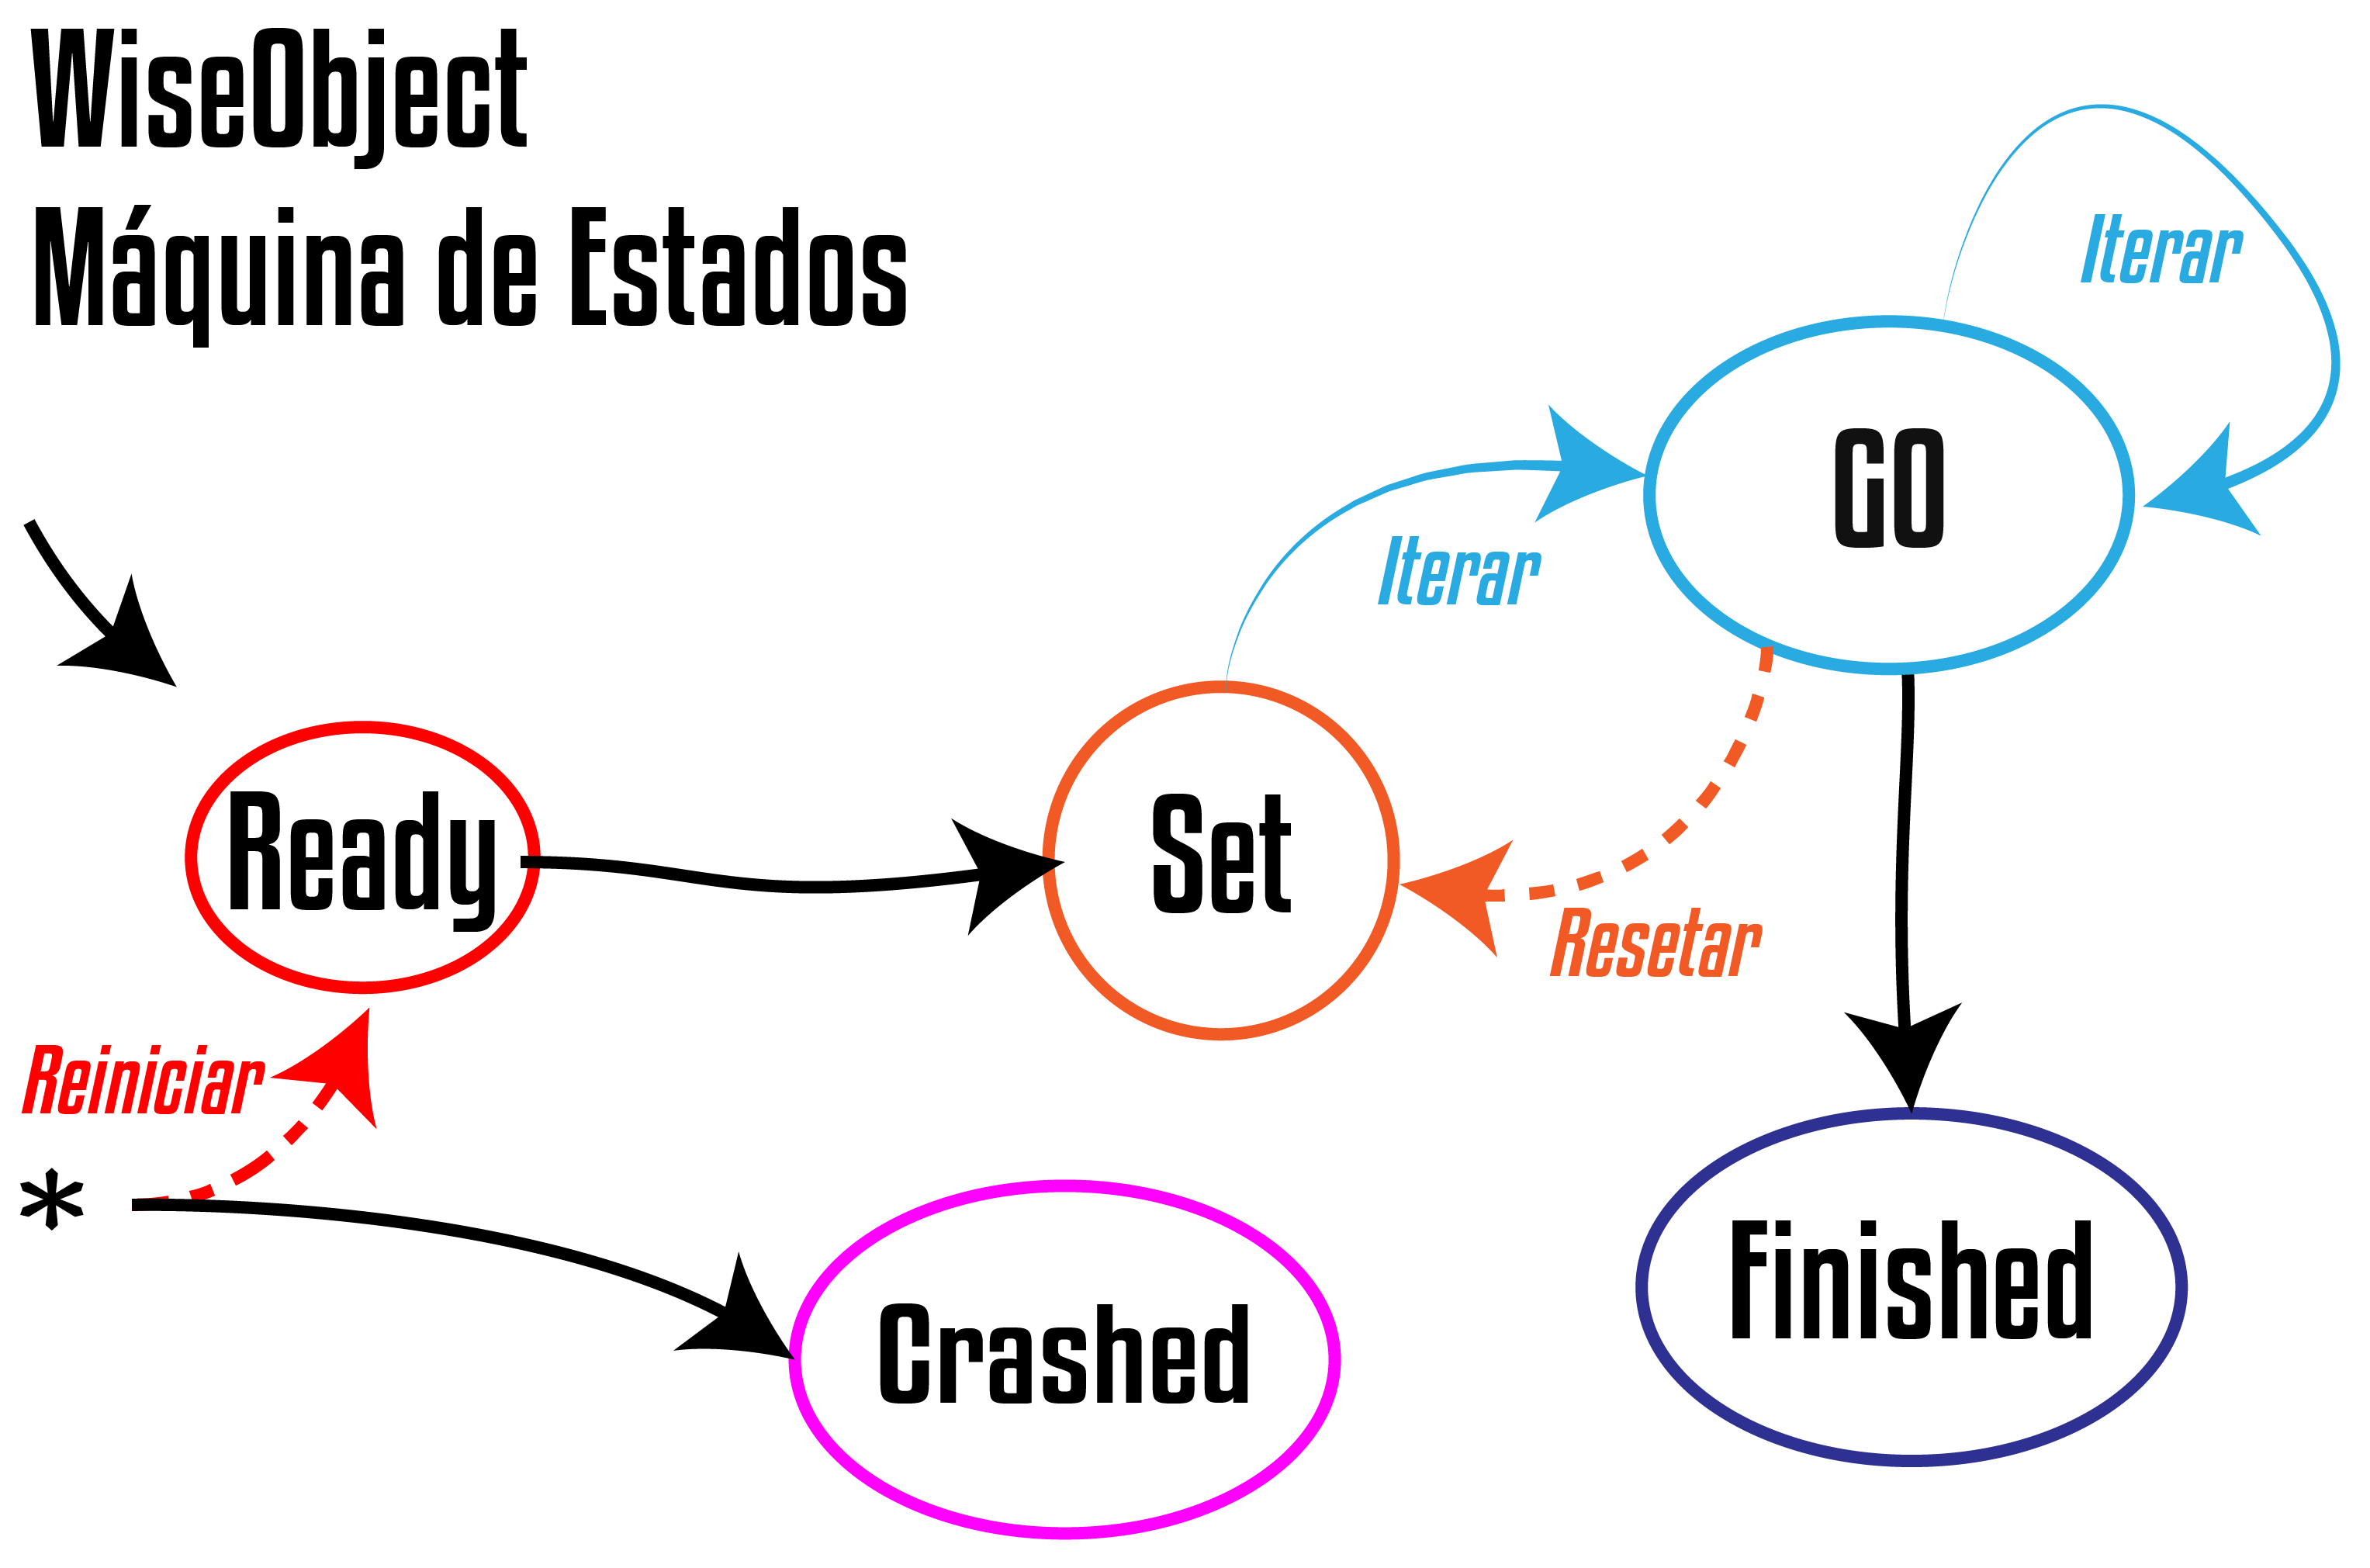
\includegraphics[width=0.6\textwidth]{Figures/WiseObjectStatus@16x.png}
		
	\end{center}
	
	\framebreak
	
	\begin{itemize}
		\item Todas as transições de estados e as ações que podem ser executadas sobre um objeto inteligente são interações do usuário. Ao se criar o objeto somente o elemento inicial e sua cópia estarão presentes no \textit{Forno} e no \textit{Freezer}, respectivamente.
		\item No estado inicial \textit{Ready} o objeto é capaz de incluir suas fábricas de iteração e gráficas.
		\item Após a inclusão de uma fábrica de iteração o objeto pode avançar para o estado \textit{Set}. Neste estado os parâmetros de iteração são adicionados à estrutura \textit{WiseStructure} e podem ser editados pelo usuário, parâmetros como frequência, viscosidade e ângulo de fase.
		\item Pode-se arbitrariamente definir o fim das iterações e enviar o objeto para o estado \textit{Finished}, que impossibilitará o objeto de continuar iterando.
		\item Finalmente, todos os estados podem levar ao estado \textit{Crashed} que indica o mau funcionamento do objeto.
	\end{itemize}
	
	\framebreak
	
		\begin{itemize}
				\item Com todas as estruturas básicas definidas, o pacote de classes que organiza or objetos e elementos inteligentes e suas necessidades intitula-se \textit{WiseThreadPool}.
		\end{itemize}		
	
	\begin{center}
		
		\item 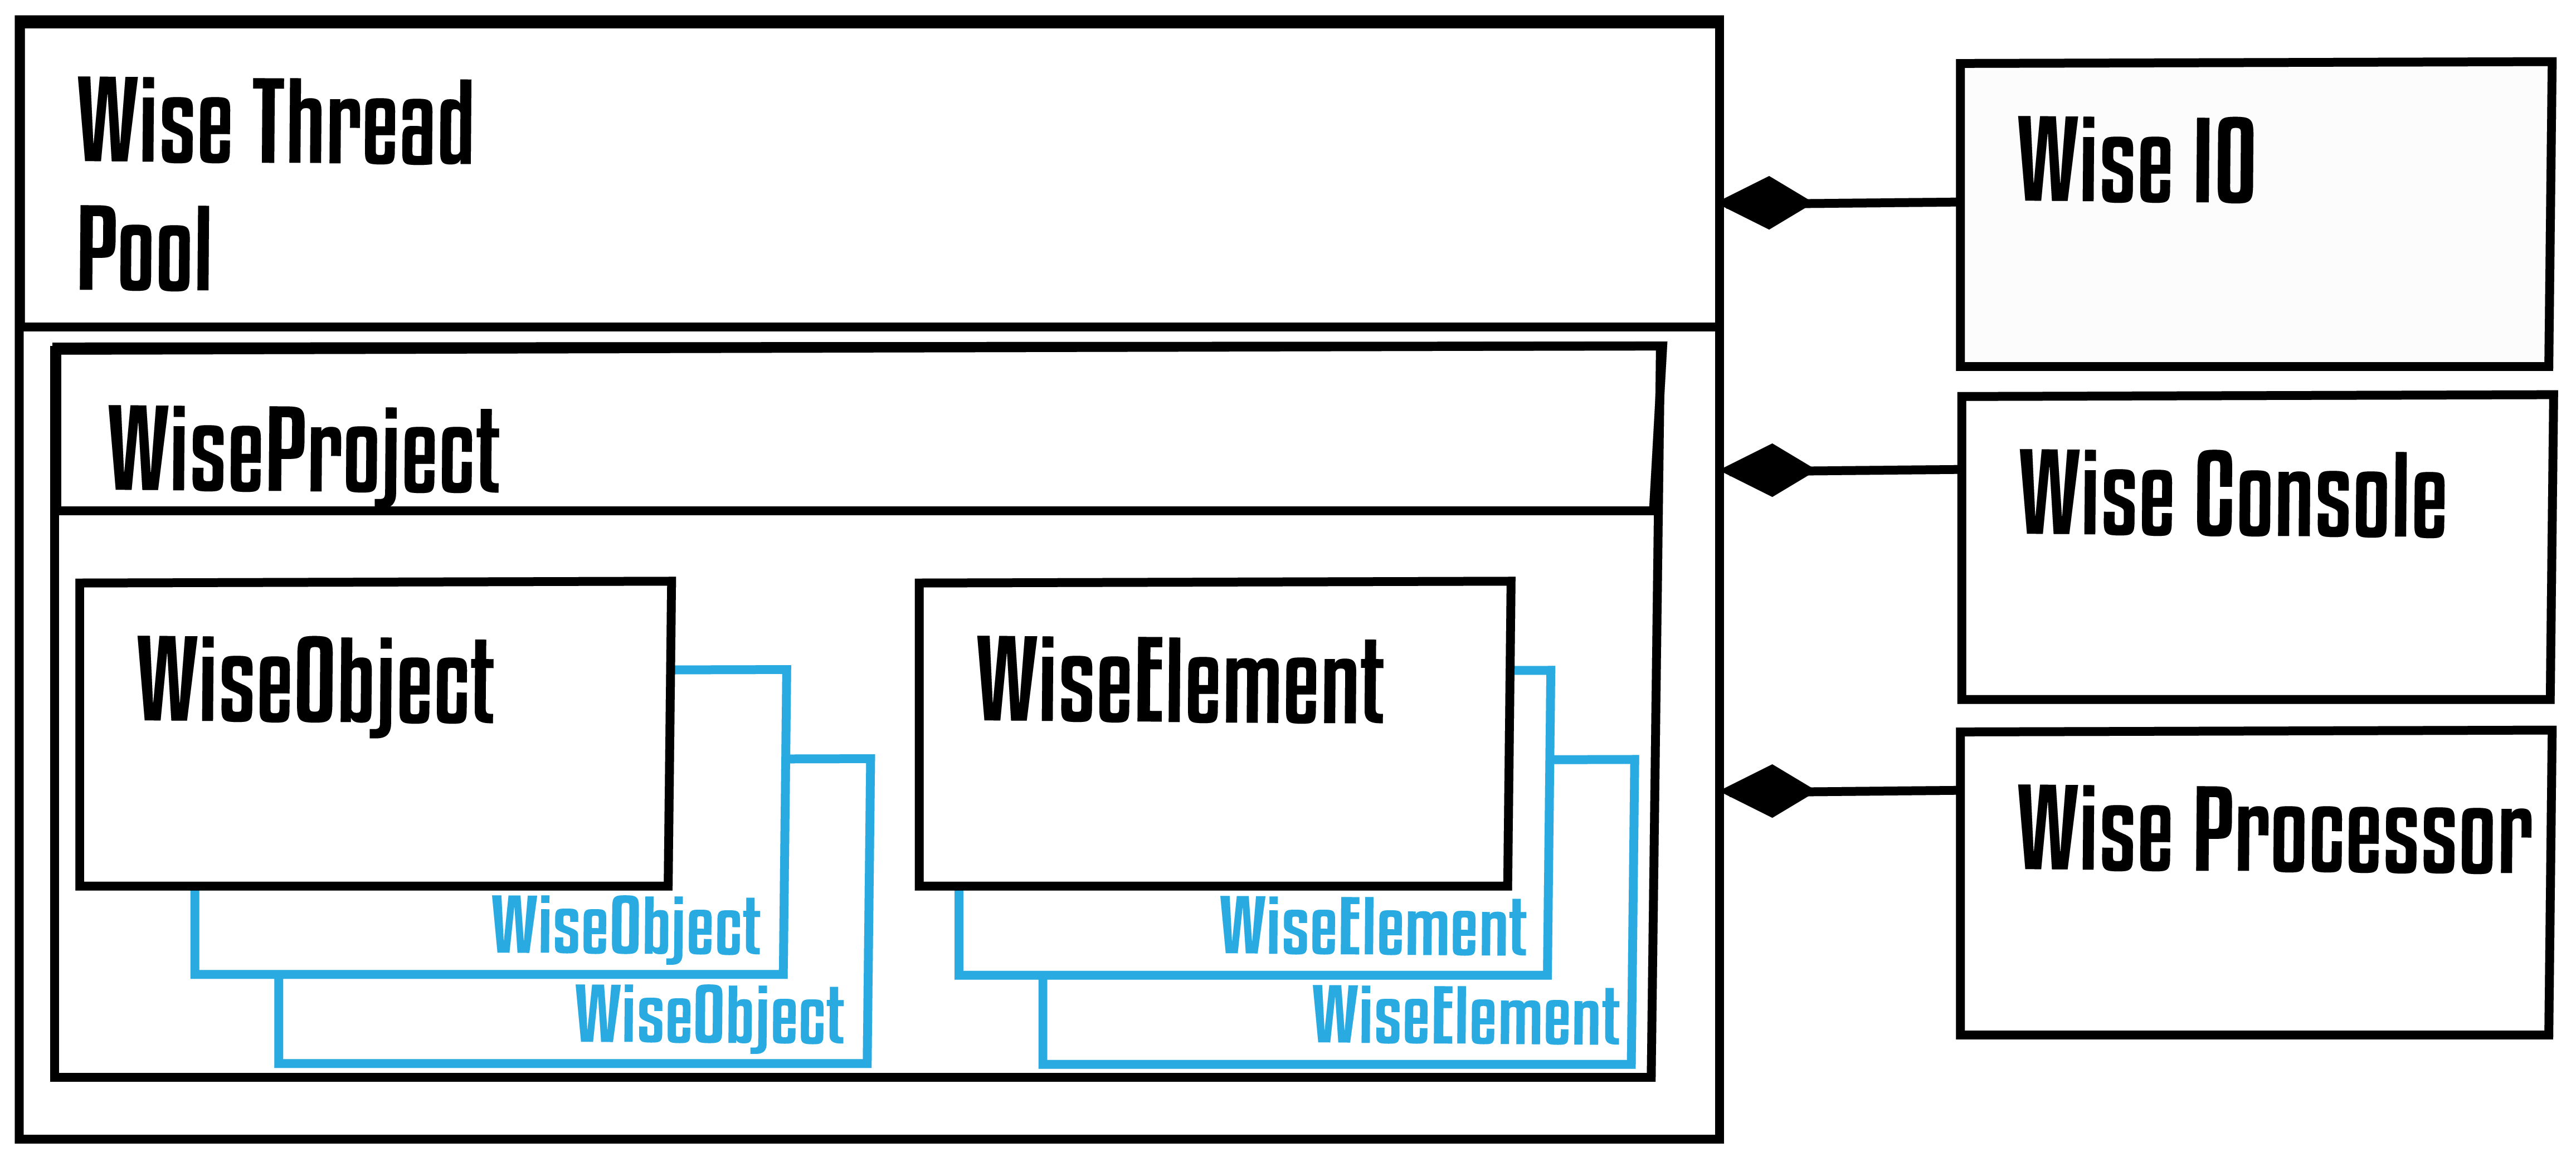
\includegraphics[width=0.6\textwidth]{Figures/WiseThreadPool@16x.png}
		
	\end{center}
	
	\framebreak
	
	\begin{itemize}
		\item Os objetos e elementos inteligentes organizam-se em projetos inteligentes, \textit{WiseProject}.
		\item A classe \textit{WiseThreadPool} é responsável por alocar estes projetos e receber suas demandas, resfriar ou aquecer objetos. É responsável também pelas demandas feitas pelo usuário através de linhas de comando.
	\end{itemize}
	
	\framebreak
	
	\begin{itemize}
		\item Cada uma das classes à seguir está contida em uma \textit{thread} própria e tem o próprio \textit{loop} de iteração.
	\end{itemize}		
	
	\begin{center}
		
		\item 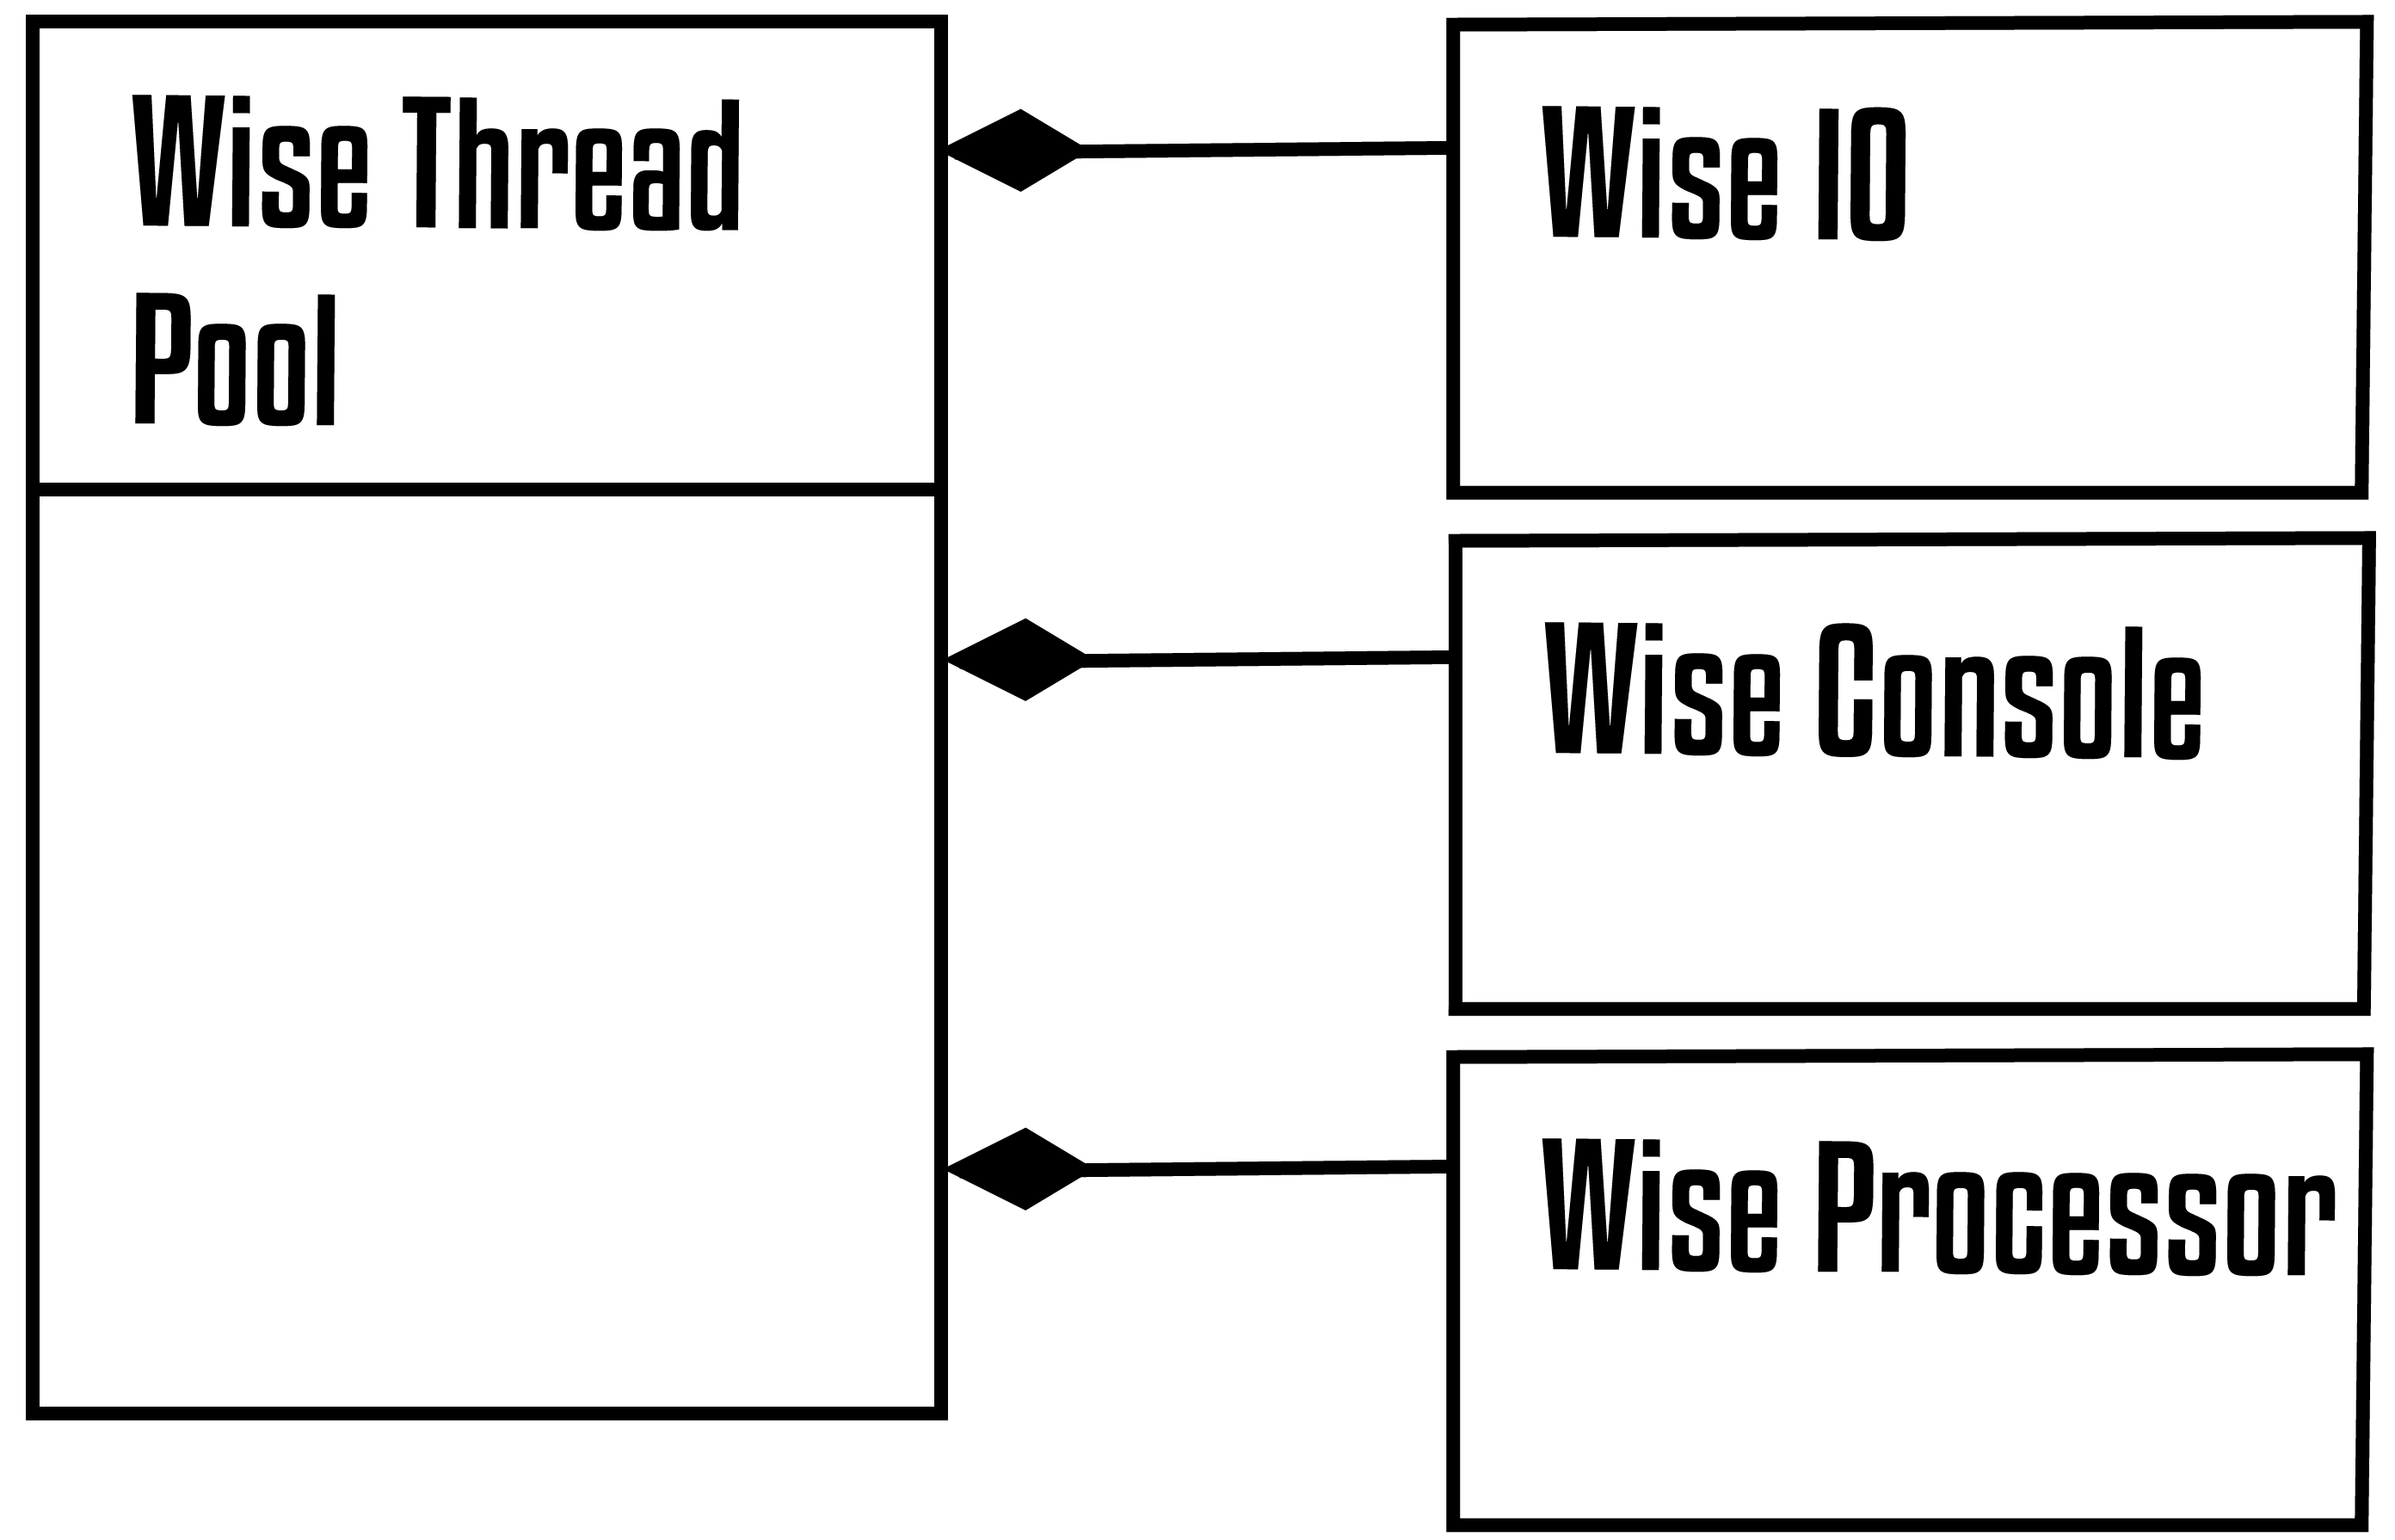
\includegraphics[width=0.6\textwidth]{Figures/WiseThreadPool2@16x.png}
		
	\end{center}
	
	\framebreak

	\begin{itemize}
		\item Ao receber uma linha de comando o objeto \textit{WiseThreadPool} enviar a mensagem e o projeto atual à uma instância de \textit{WiseConsole}, que é responsável por interpretar o comando.
		\item Caso seja um processo que utilize o disco rígido, uma instância \textit{WiseIO} será necessária para executar o comando. 
		\item Caso seja um processo de iteração, uma instância \textit{WiseProcessor} será utilizada.
		\item Para os restantes dos casos a própria classe \textit{WiseConsole} será utilizada para finalizar o comando. A alteração de parâmetros ou sua escala cai neste último caso.
	\end{itemize}		
	
	\begin{center}
		
		\item 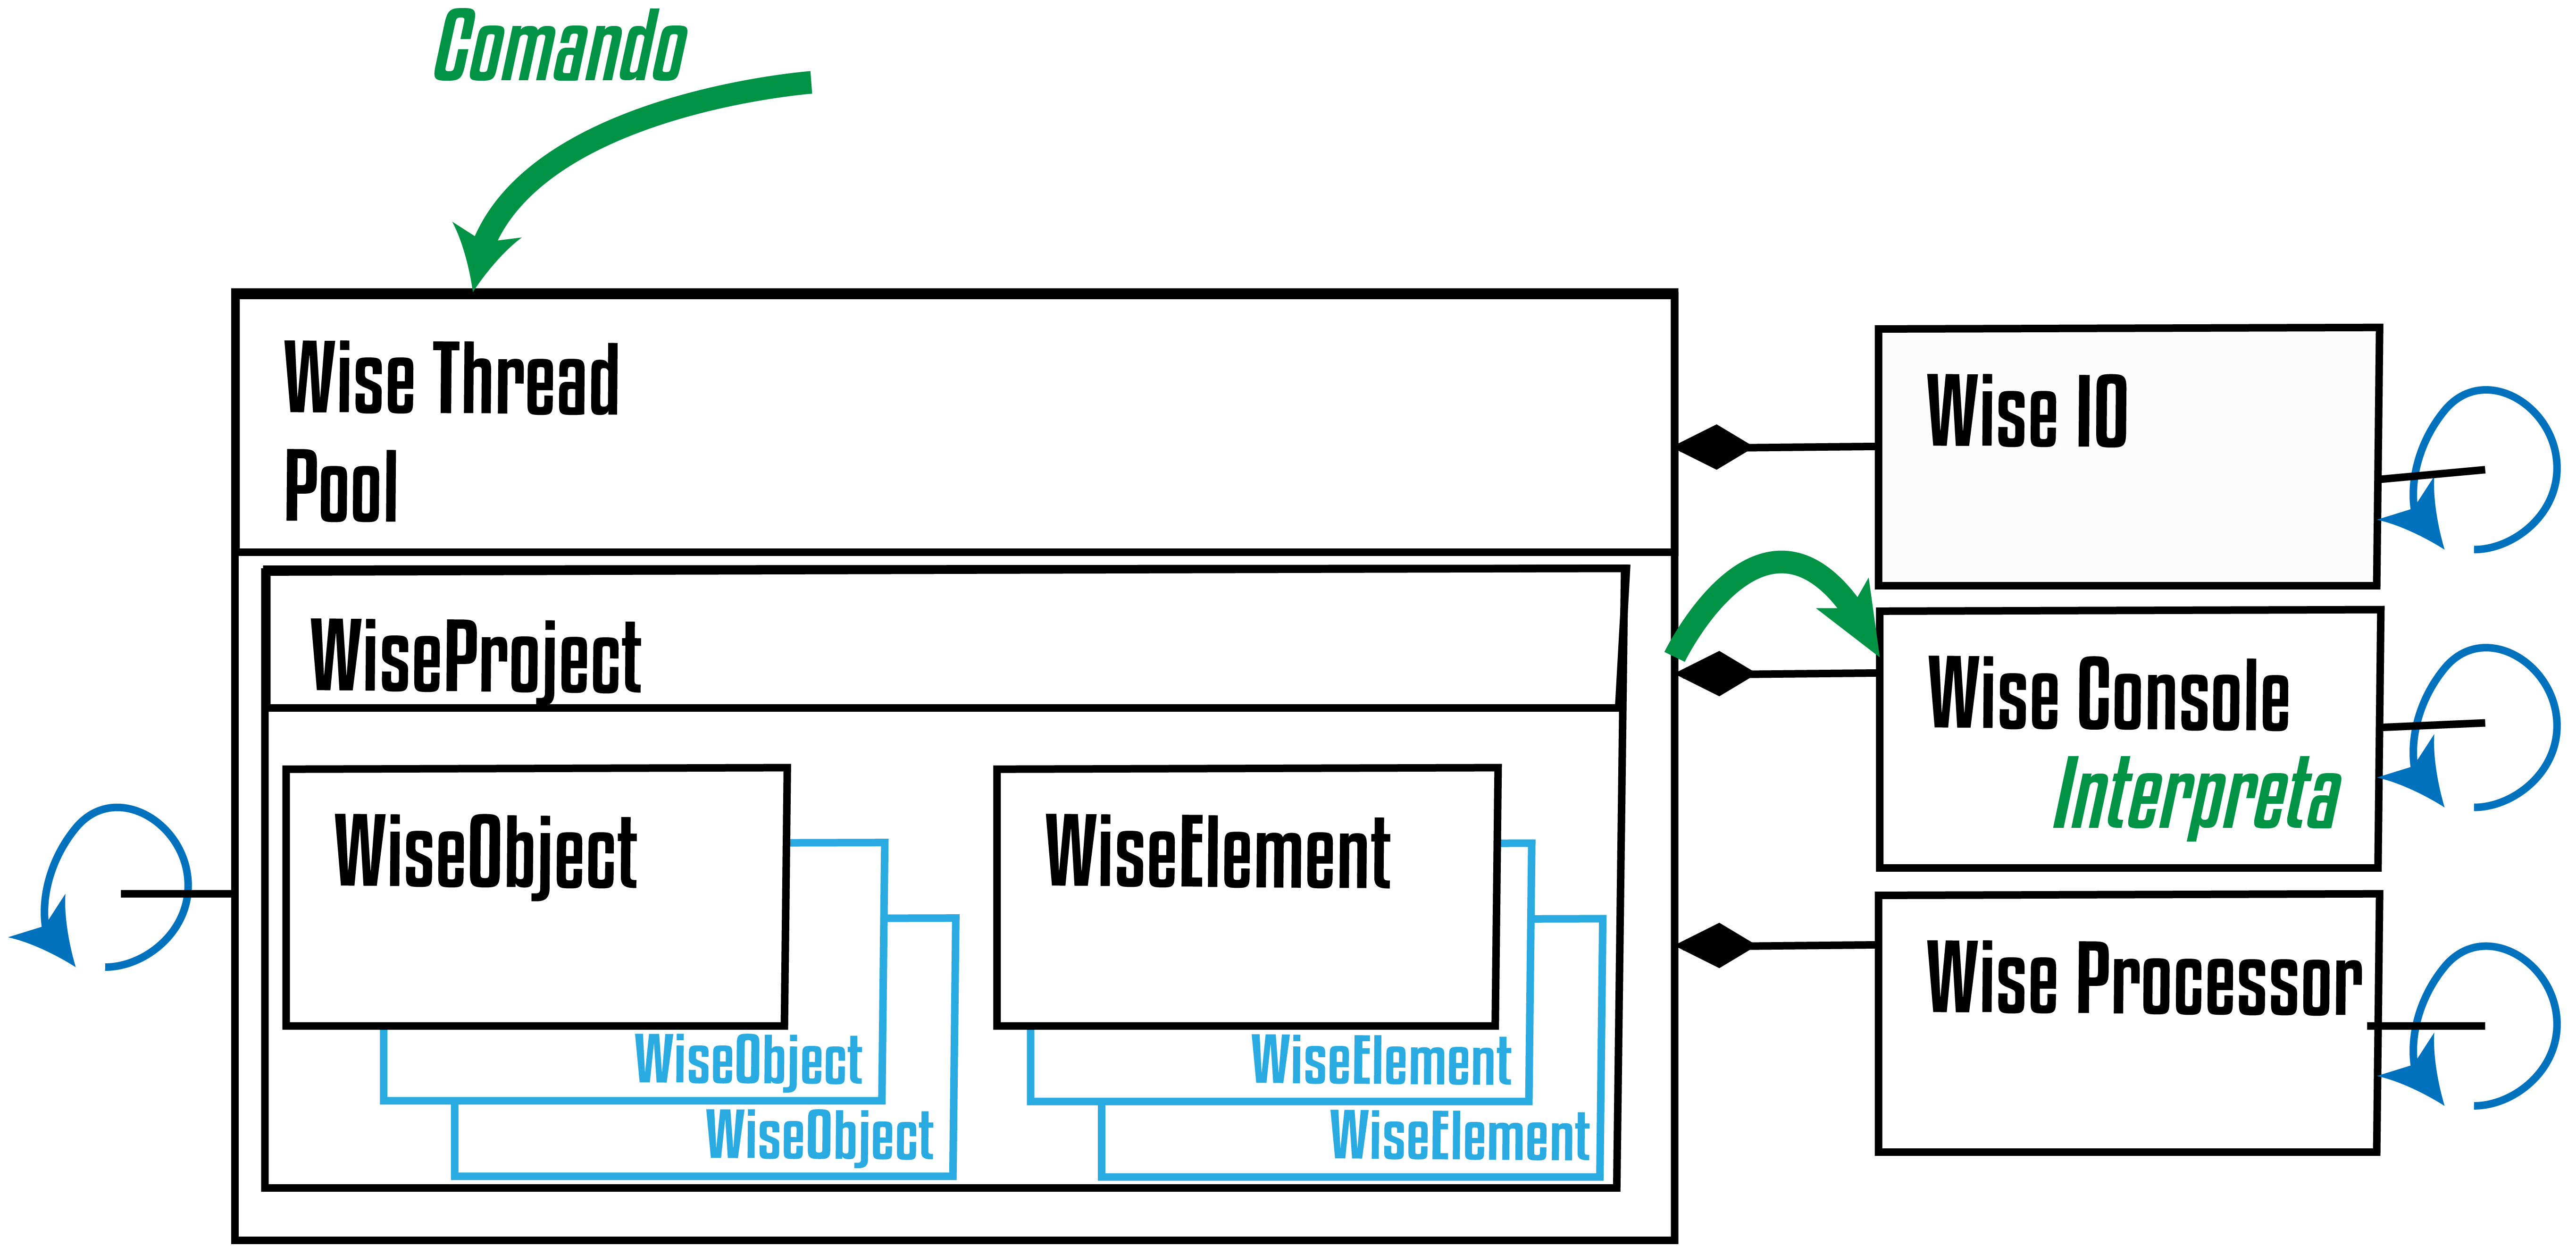
\includegraphics[width=0.6\textwidth]{Figures/WiseThreaPoolCMD@16x.png}
		
	\end{center}
	
	\framebreak
	\begin{center}
		
		\item \includegraphics[width=0.6\textwidth]{Figures/WiseThreaPoolCMDSub@16x.png}
		
	\end{center}
	
	\framebreak
	
	\begin{itemize}
			\item O resfriamento ou aquecimento de elementos envolve sempre uma instância de \textit{WiseIO}.
	\end{itemize}		
	
	\begin{center}
		
		\item 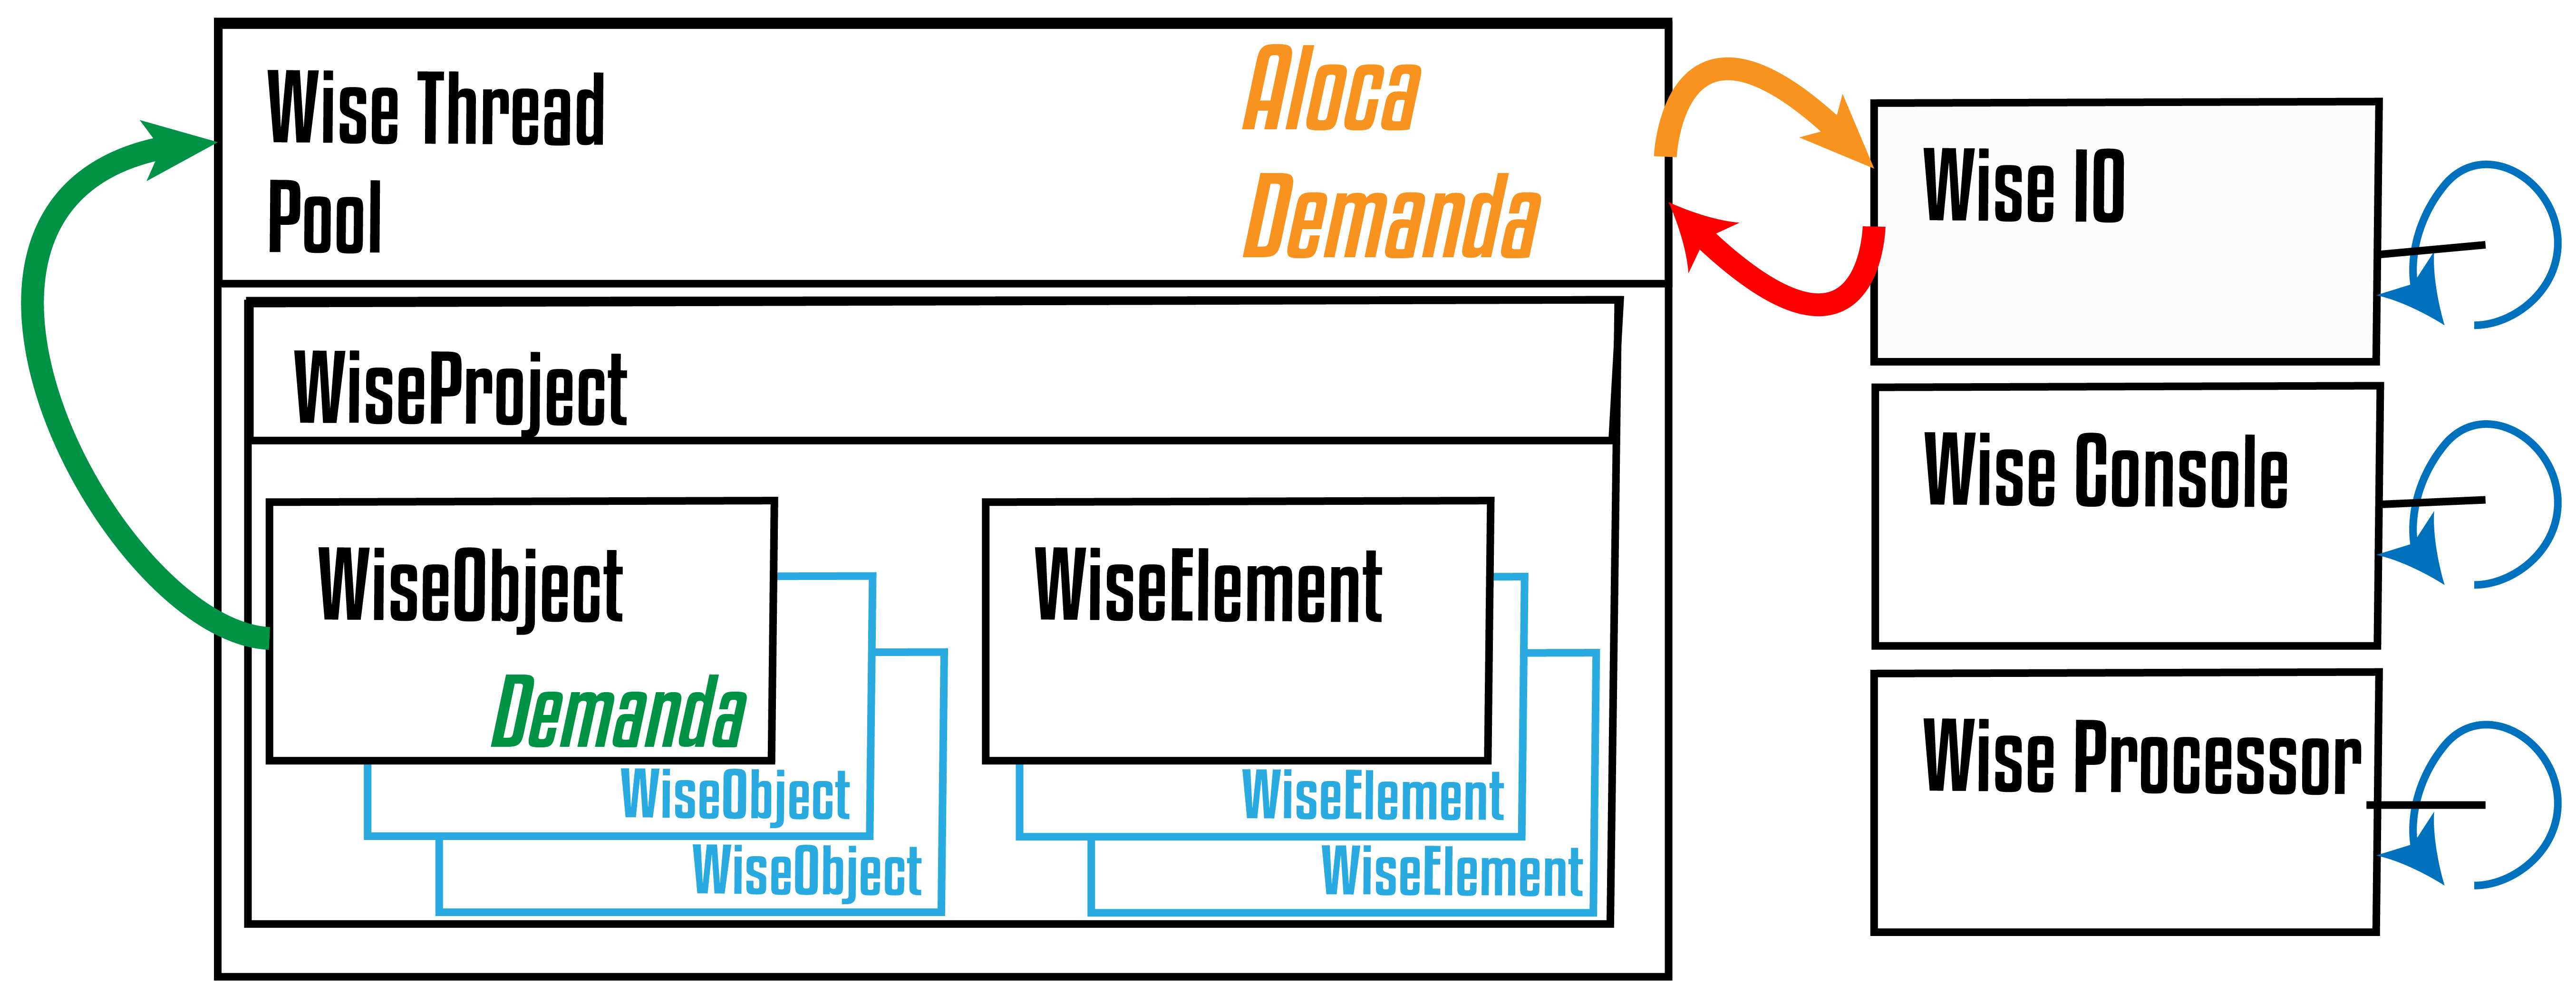
\includegraphics[width=0.6\textwidth]{Figures/WiseThreadPoolHeating@16x.png}
		
	\end{center}
	
	\framebreak
	
	\begin{itemize}
		\item Um \textit{WiseThreadPool} irá conter todas as instâncias de \textit{WiseIO}, \textit{WiseConsole} e \textit{WiseProcessor} e está preparado para utilizar mais de uma instância destes objetos por vez.
		\item Essencialmente isto significa que os objetos e elementos armazenados pelo projeto inteligente, \textit{WiseProject}, podem ser acessados pelos diferentes processadores independentemente.
		
		\item Isto dá ao usuário uma imensa liberdade na hora de decidir executar algum algoritmo concorrentemente, entretanto requer cuidados especiais na hora de utilizar os objetos.
		
		\item Como os objetos podem ser acessados por mais de um processador, eles são bloqueados por uso.
	\end{itemize}

\end{frame}
		
		
\section{Ferramenta Computacional}
\begin{frame}[allowframebreaks]
\frametitle{Ferramenta Computacional}		
	\begin{itemize}
		\item Com a estrutura de dados definida a ferramenta foi dividida em dois ambientes:
		\item  A interface gráfica \textit{\textbf{IGU}} (\textbf{I}nterface \textbf{G}ráfica \textbf{U}niversal), que representa o ambiente gráfico da ferramente.
		\item  E, o console \textit{\textbf{InGU}}(\textbf{I}nterface \textbf{n}ão-\textbf{G}ráfica \textbf{U}niversal), que é um ambiente executado sem interface gráfica e recebe comandos via texto.
	\end{itemize}

	\framebreak
	
	\begin{center}
		\begin{itemize}
		\begin{multicols}{2}
				\vfill
				\item O ambiente \textbf{IngU} ao ser executado imprime no console o cabeçalho do programa e carrega os elementos previamente carregados na ferramenta.
				\columnbreak
				\item 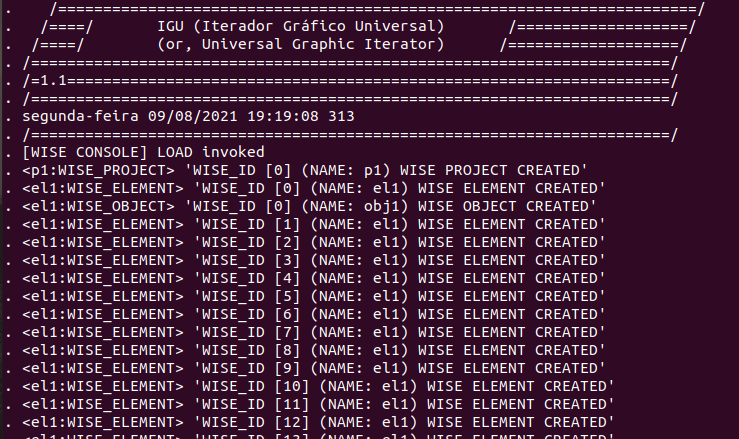
\includegraphics[width=0.5\textwidth]{Figures/InGU_console.png}
			\end{multicols}
		\end{itemize}
	\end{center}

	\framebreak
	
	\begin{itemize}
		\item O comando de ajuda é o primeiro comando da interface e foi feito para listar todas as entradas possíveis do programa.
		\item Ao receber este comando a thread \textit{WiseConsole} envia o texto pré-definido com todos os comandos.
	\end{itemize}
	
	
	\begin{center}
		\begin{table}[!htbp]
			\begin{tabular}{|c|m{0.6\textwidth}|}
				\hline
				\textbf{Linha de Comando} & \multicolumn{1}{c|}{help} \\
				\hline
				\textbf{Escopo} & \multicolumn{1}{c|}{nenhum} \\
				\hline
				\textbf{Thread Responsável} & \multicolumn{1}{c|}{WiseConsole} \\
				\hline
				\textbf{Entrada} & Nenhuma \\
				\hline
			\end{tabular}
			\caption{Descrição do comando ajuda.}
			\label{tab:help}
		\end{table}
	\end{center}

	\framebreak

	Assim como o comando de criação de elementos inteligentes, o comando de criação de objetos irá acessar a fábrica de elementos inteligentes \textit{WiseElementFactory}. É possível criar objetos inteligentes de duas formas: A primeira, utilizando um elemento inteligente; A segunda utilizando os exemplos disponibilizados pela fábrica de elementos inteligentes.
	
	Assim como descrito anteriormente, ao criar um objeto inteligente, um elemento inteligente é adicionado à estrutura do \textit{Forno}, enquanto um Clone é acoplado ao \textit{Freezer};
	
	\begin{center}
		\begin{table}[!htbp]
			\begin{tabular}{|c|c|m{0.5\textwidth}|}
				\hline
				\multirow{3}{*}{\textbf{Linha de Comando}} & \multicolumn{2}{c|}{object create <object\underline{\space\space}name> <element\underline{\space\space}name>} \\
				& \multicolumn{2}{c|}{object create <type> <example> <name> <element\underline{\space\space}name> [ARGS]} \\
				\hline
				\textbf{Escopo} & \multicolumn{2}{c|}{OBJECT} \\
				\hline
				\textbf{Thread Responsável} & \multicolumn{2}{c|}{WiseConsole} \\
				\hline
				\multirow{3}{*}{\textbf{Entrada}} & <object\underline{\space\space}name> & Nome do objeto à ser criado. \\
				& <element\underline{\space\space}name> & Nome do elemento à ser utilizado na criação ou do elemento à ser criado a partir do exemplo. \\
				& <type> & Tipo de elemento inteligente à ser criado. \\
				& <name> & Nome do exemplo de elemento inteligente à ser criado. \\
				& [ARGS] & Individualmente,  as fábricas podem receber parâmetros para a criação de elementos. \\
				\hline
			\end{tabular}
			\caption{Descrição do comando para criar objetos inteligentes.}
			\label{tab:create_object}
		\end{table}
	\end{center}

\end{frame}


\section{InGU}
\begin{frame}[allowframebreaks]
\frametitle{InGU}
	
	\begin{center}
	\begin{itemize}
		\begin{multicols}{2}
			\vfill
			\item O ambiente \textbf{InGU} tem como principal objetivo a iteração modelos utilizando alguma lógica pré-definida por algum algoritmo disponível. Através dos comandos disponibilizados é possível que estes modelos sejam criados, alterados, iterados e, opcionalmente, visualizados. Com isto o principal fluxo de uso foi disponibilizado.
			\columnbreak
			\item 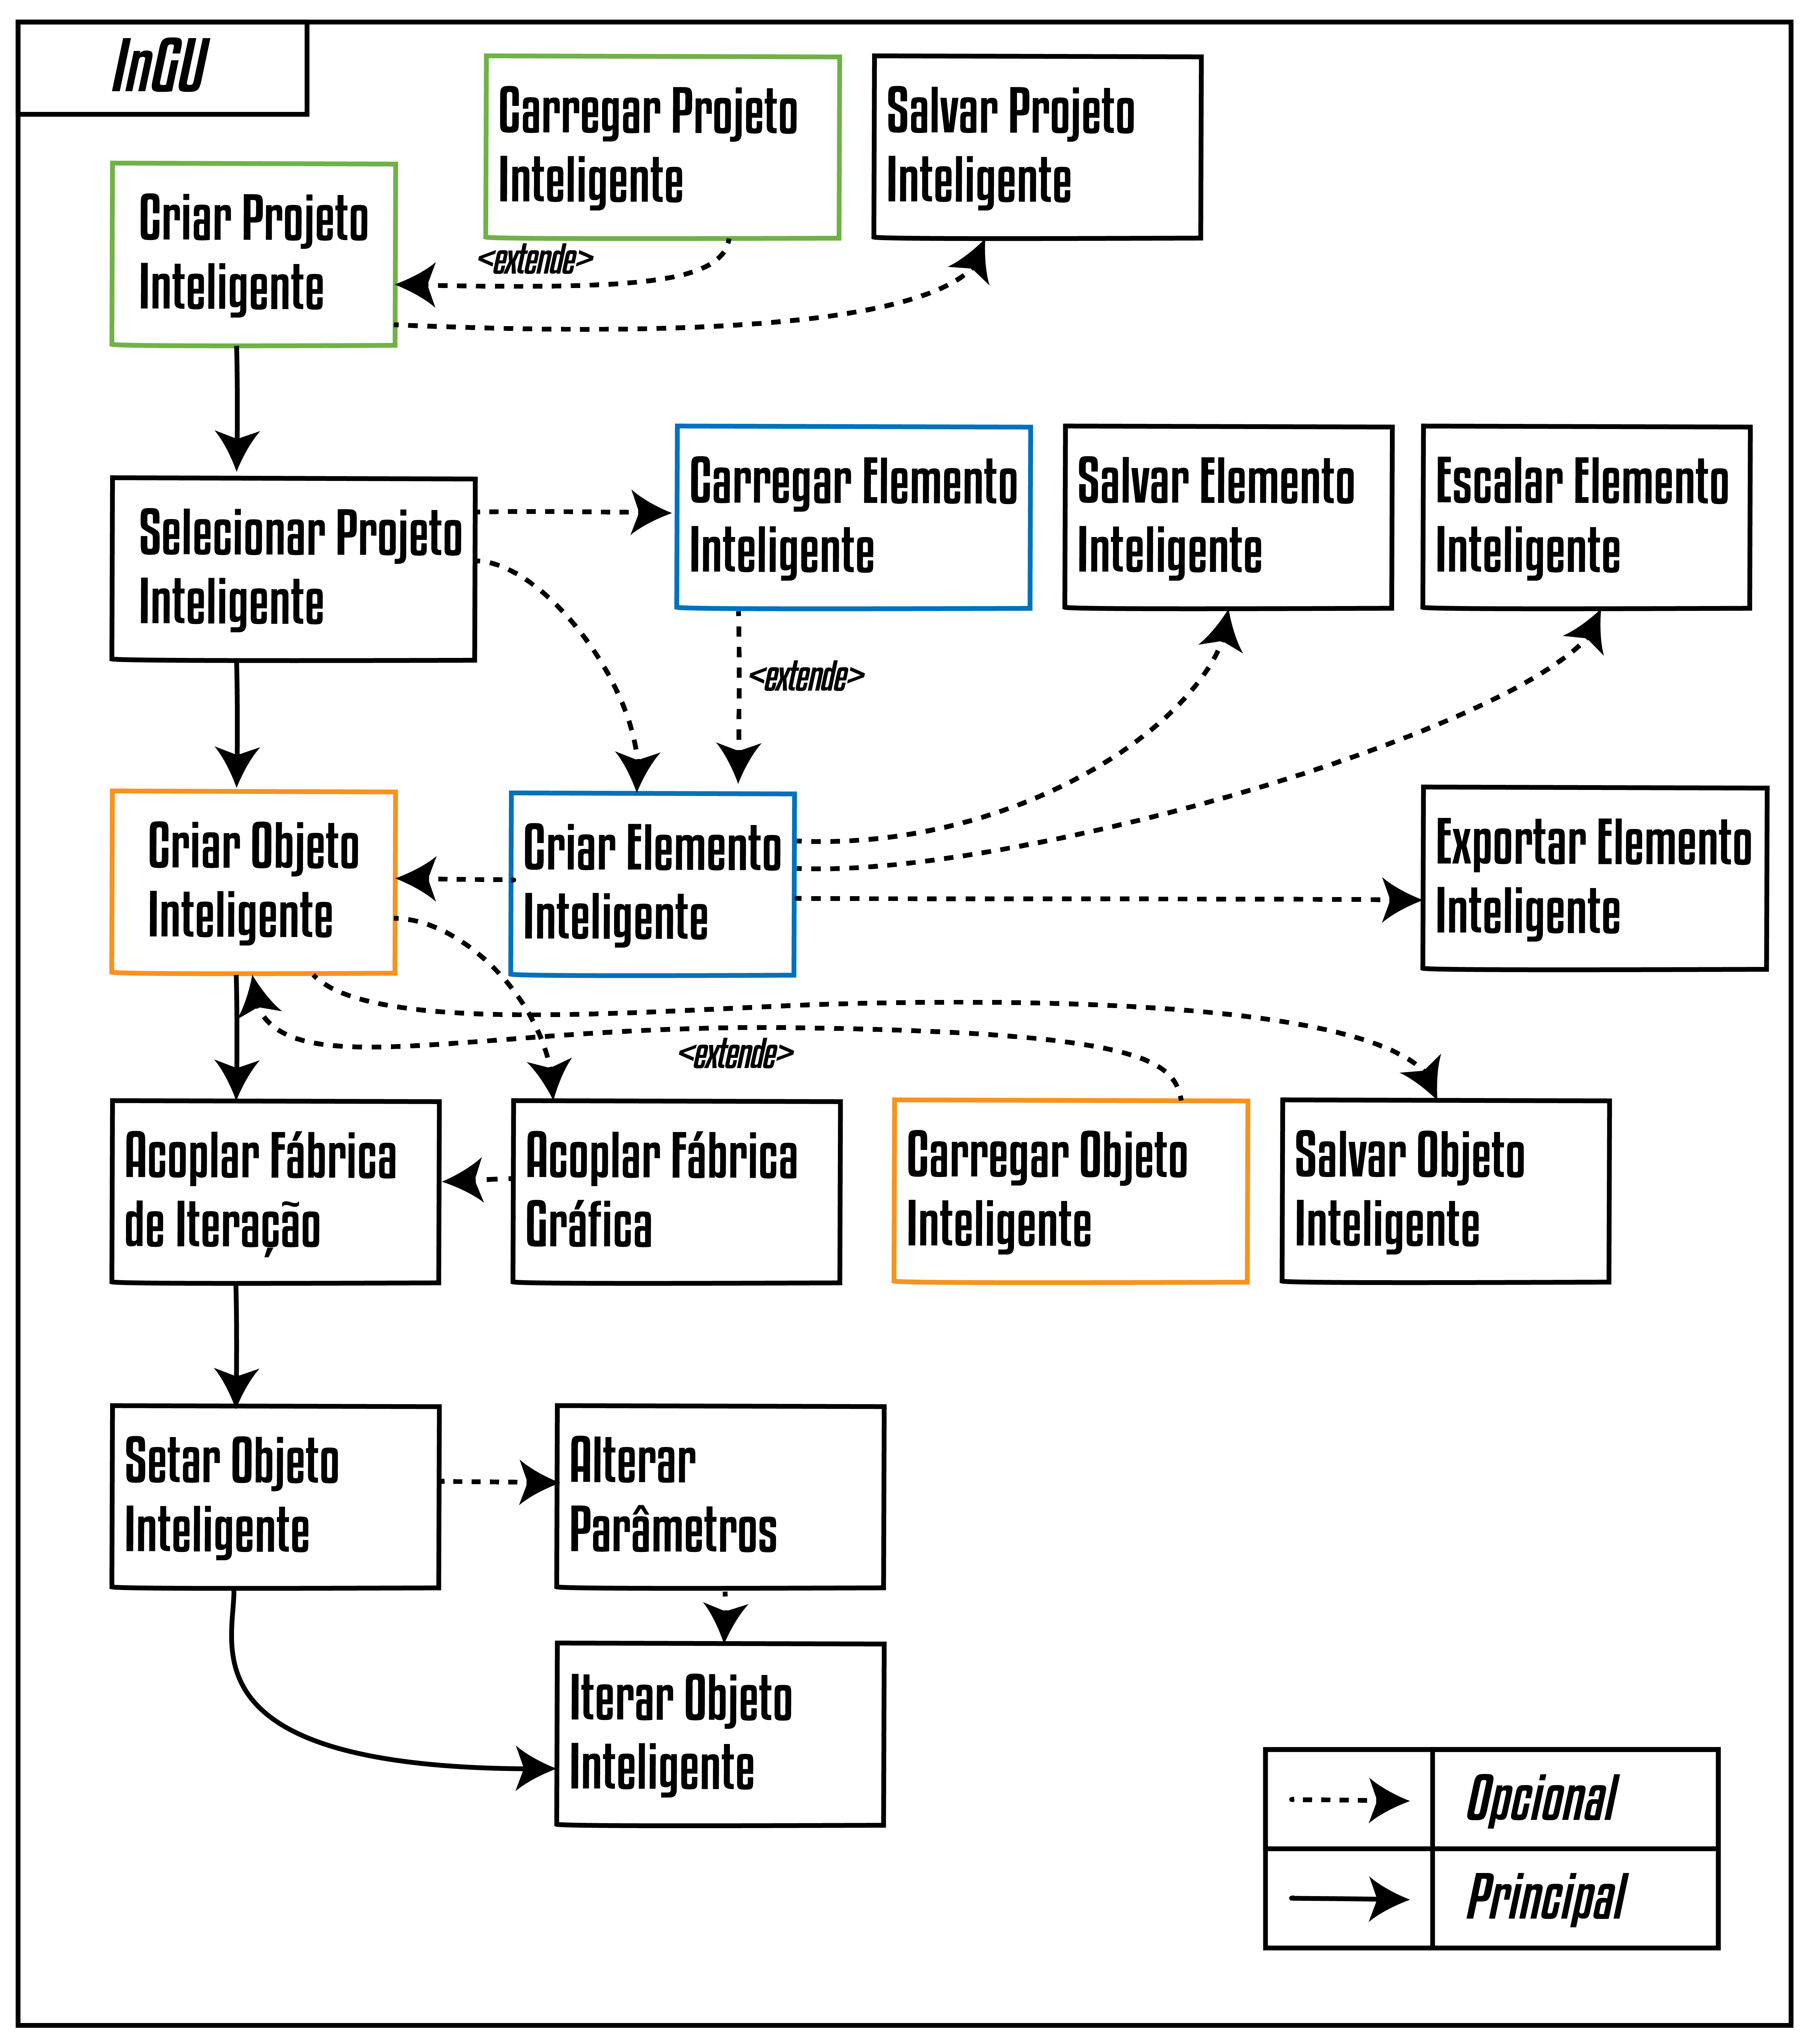
\includegraphics[width=0.45\textwidth]{Figures/CasoDeUso@16x.png}
		\end{multicols}
	\end{itemize}
	\end{center}
\end{frame}


\section{IGU}
\begin{frame}[allowframebreaks]
\frametitle{IGU}
	\begin{itemize}
		\item Já o ambiente \textbf{IGU} tem como principais objetivos possibilitar a realização do fluxo disponibilizado no ambiente \textit{\textbf{InGU}} e incorporar um interface de usuário gráfica. Através da interface de usuário é possível que estes modelos sejam criados, alterados, iterados e, opcionalmente, visualizados.
	\end{itemize}		
	
	\begin{center}
	
		\item 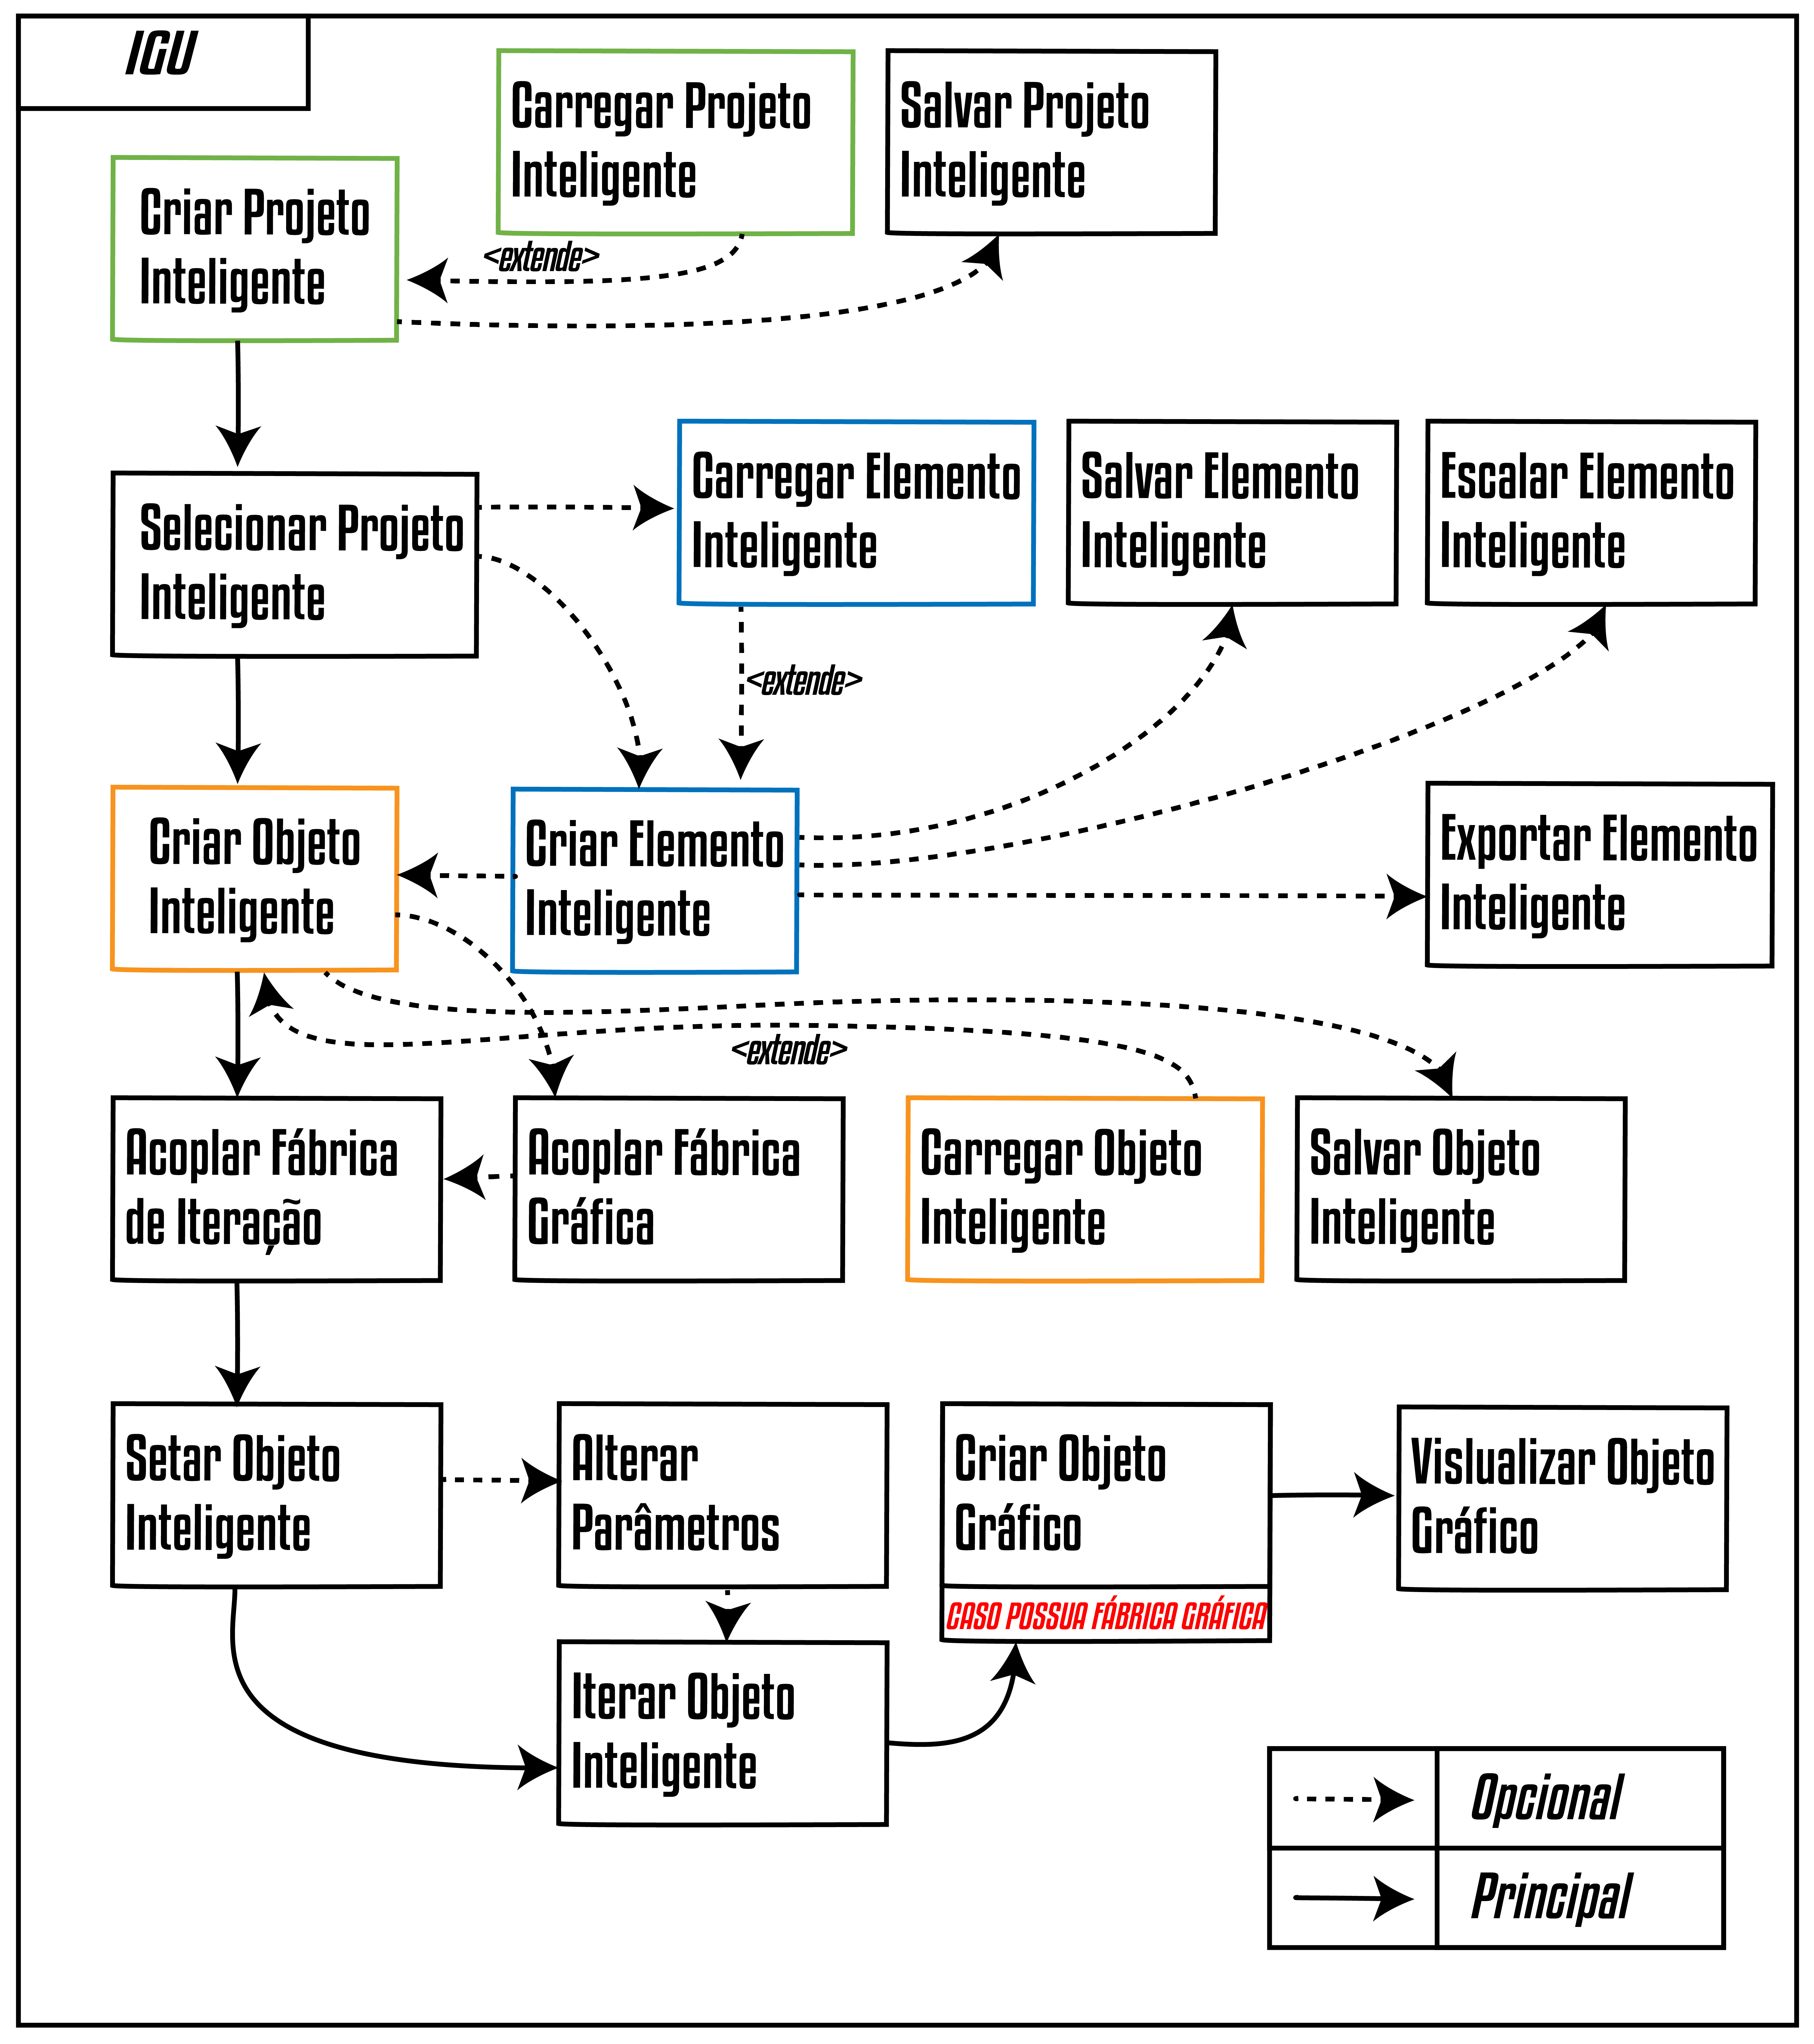
\includegraphics[width=0.45\textwidth]{Figures/CasoDeUso2@16x.png}
		
	\end{center}
	
	\framebreak
	
	\begin{itemize}
		\item A janela principal do ambiente computacional \textit{\textbf{IGU}} é composta por: 1. Menu principal do programa; 2. Árvore de projetos e seus elementos; 3. Área de trabalho, no caso mostrando OpenGl \textit{Canvas}; 4. Seleção de abas.
	\end{itemize}		
	
	\begin{center}
		
		\item 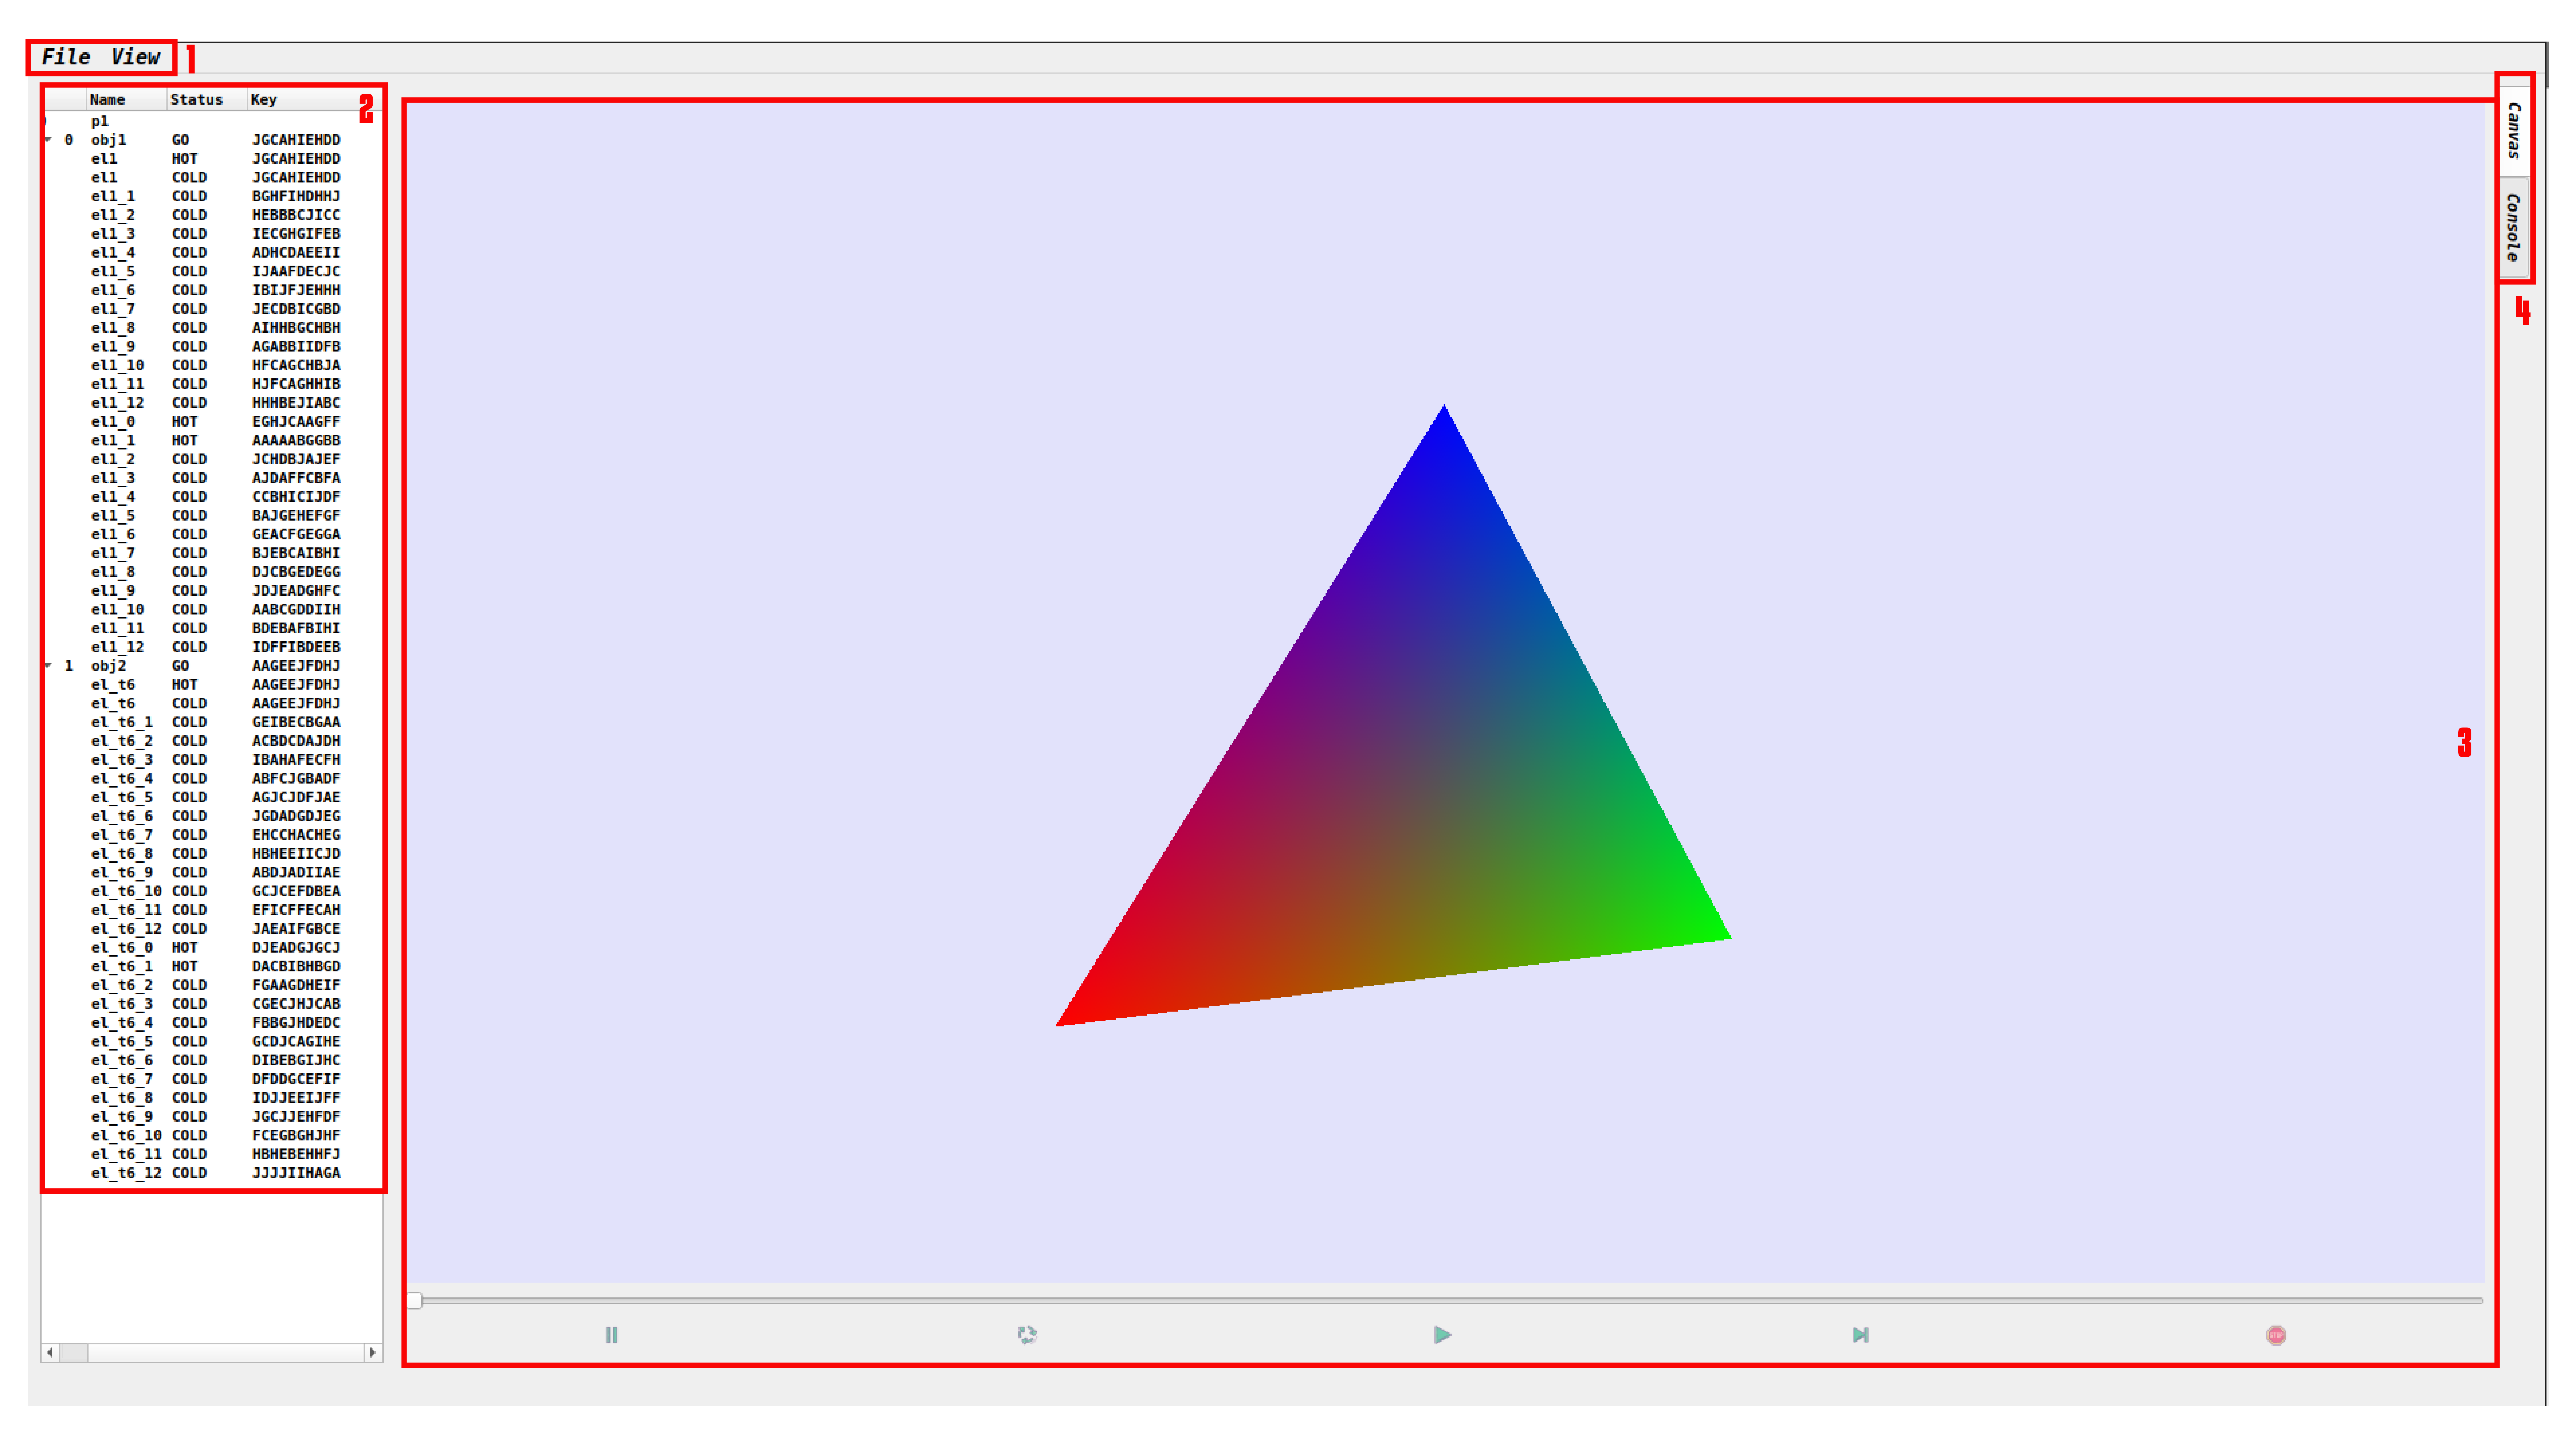
\includegraphics[width=0.6\textwidth]{Figures/IGU_001a.png}
	
	\end{center}
	
	\framebreak
	
	\begin{center}
	\begin{itemize}
		\begin{multicols}{2}
			\vfill
			\item O primeiro grupo são os elementos que compões o menu principal da aplicação. Cada opção do menu é representada por um uma linha de texto, ao selecionar a linha uma ação é executada:
			\item \textbf{Exit}: Fecha o ambiente computacional.
			\item \textbf{Jobs}: Abre a Janela que exibe os trabalhos inteligentes criados.
			\item \textbf{Open Canvas}: Abre uma nova janela contendo um novo elemento gráfico OpenGL \textit{Canvas}.
			\columnbreak
			\item 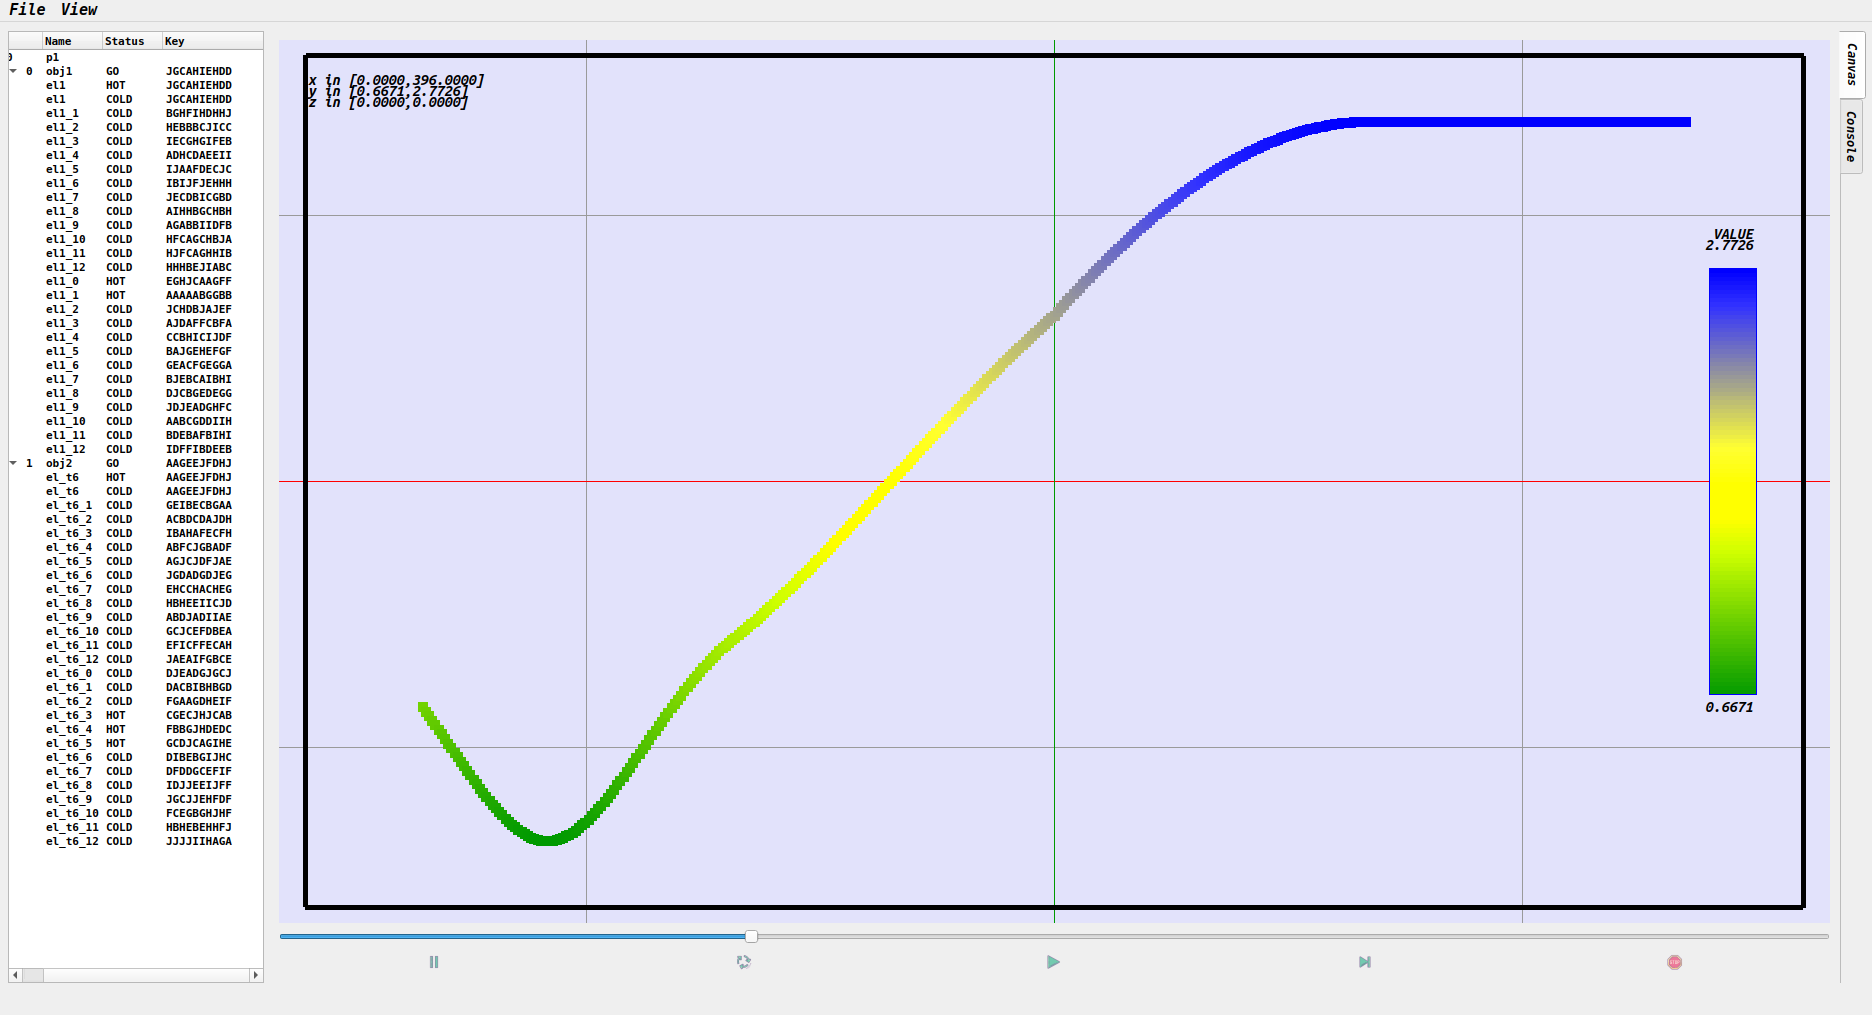
\includegraphics[width=0.5\textwidth]{Figures/IGU_016.png}
		\end{multicols}
	\end{itemize}
	\end{center}

	\framebreak
	
	\begin{center}
		\begin{itemize}
			\begin{multicols}{2}
				\vfill
				\item Ao selecionar uma das abas, os elementos de interface de usuário da área de trabalho são trocados. Estes elementos são objetos do tipo \textit{QWidget}, estes objetos que são divididos em dois ambientes, o \textit{Canvas} e o \textit{Console}. 
				
				\item Ao selecionar a opção do \textit{Console} um ambiente similar ao disponibilizado pelo ambiente \textit{InGU} é disponibilizado. 
				\columnbreak
				\item 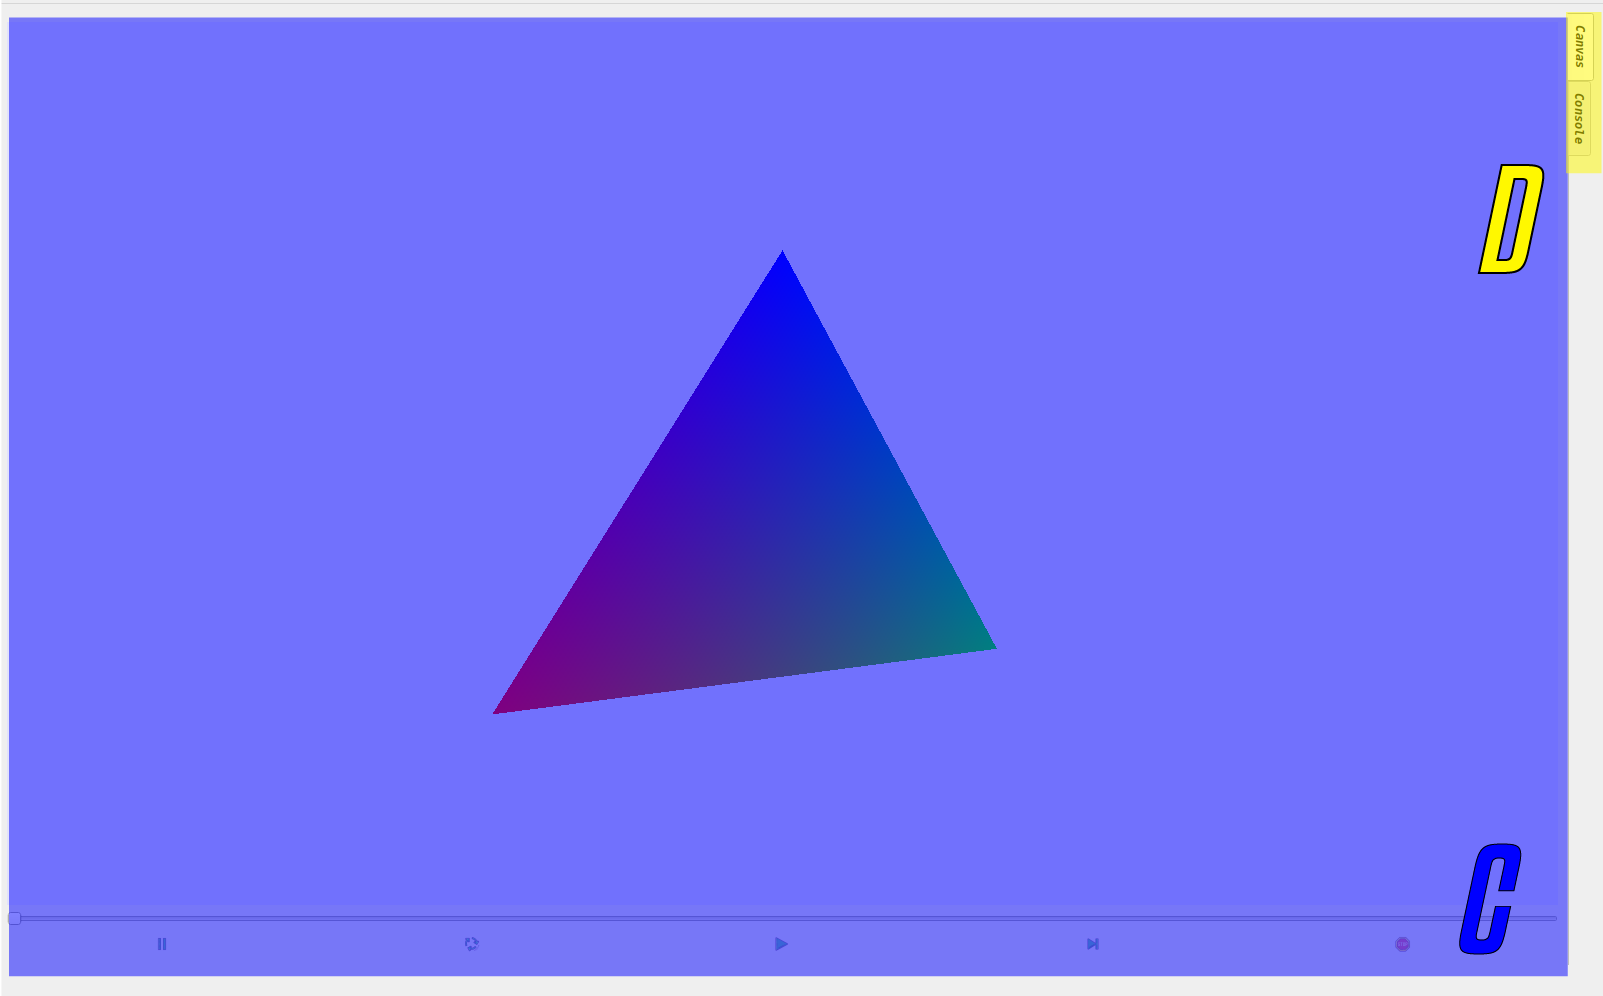
\includegraphics[width=0.5\textwidth]{Figures/IGU_001a_34.png}
			\end{multicols}
		\end{itemize}
	\end{center}

	\framebreak
	
	\begin{center}
	\begin{itemize}
		\begin{multicols}{2}
			\item 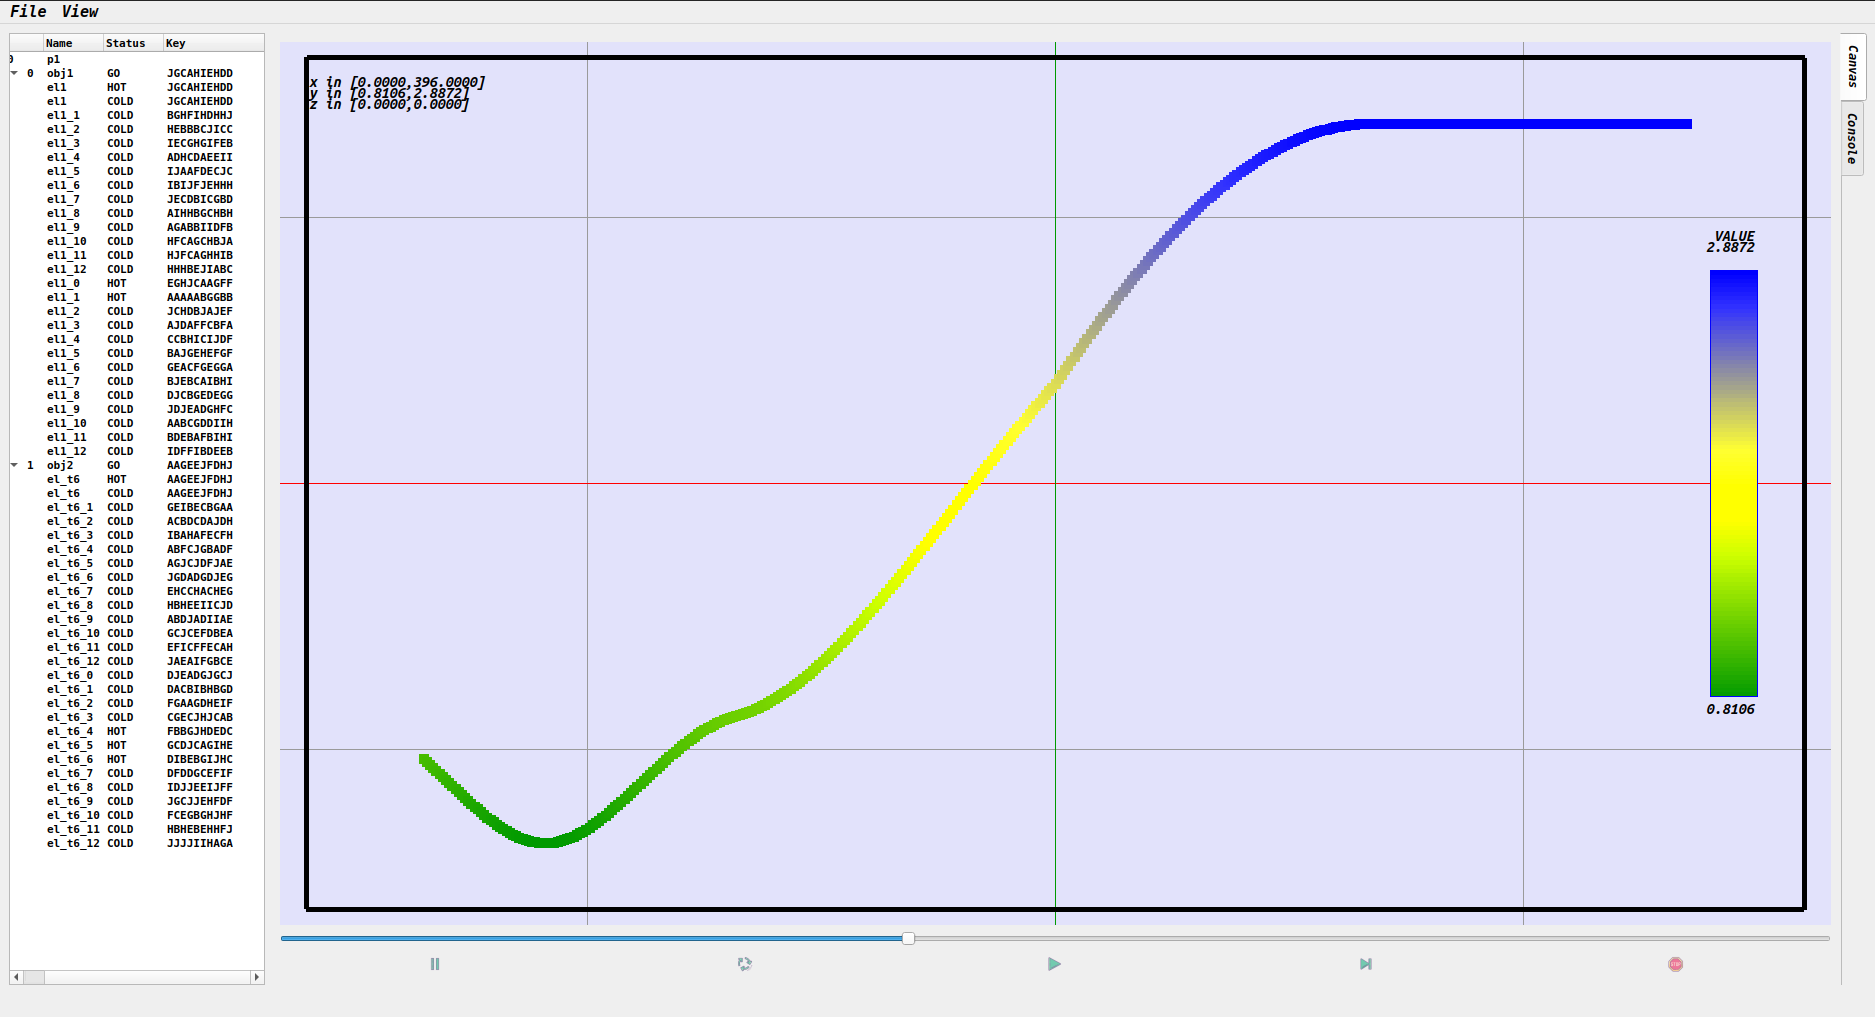
\includegraphics[width=0.5\textwidth]{Figures/IGU_017.png}
			\columnbreak
			\item 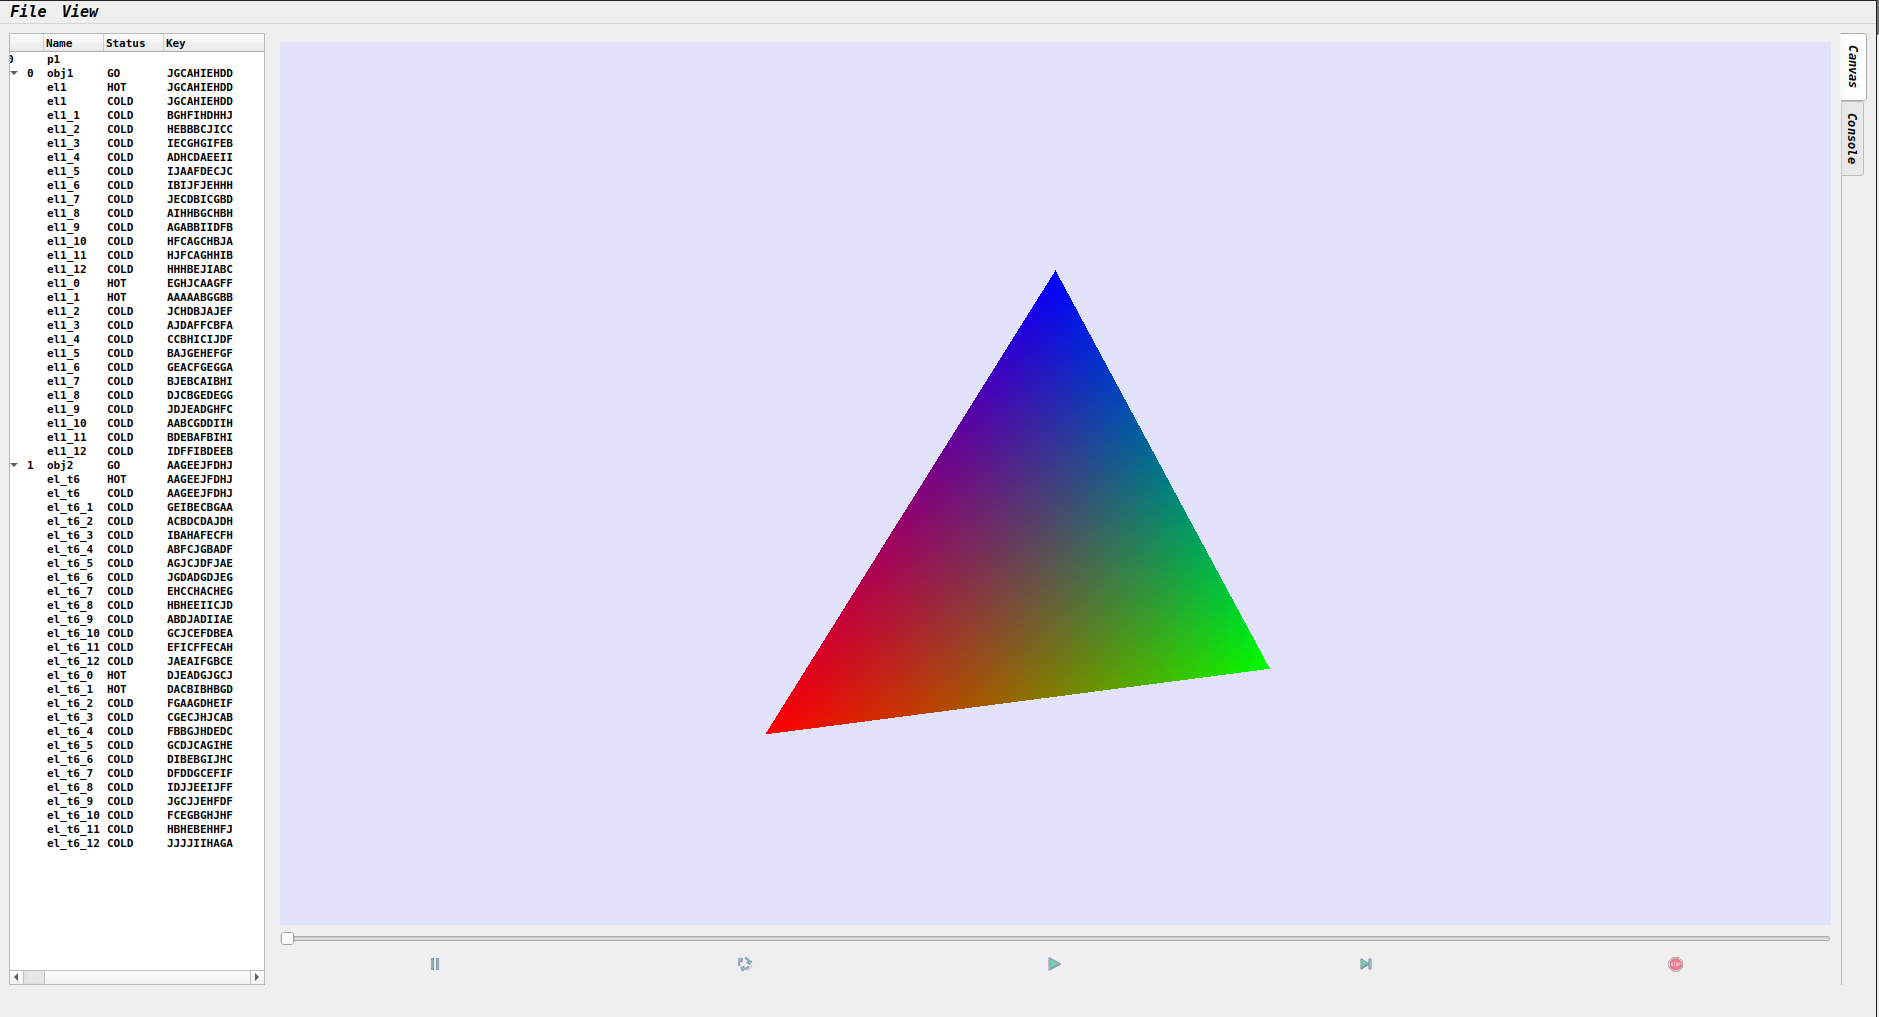
\includegraphics[width=0.5\textwidth]{Figures/IGU_001.png}
		\end{multicols}
	\end{itemize}
	\end{center}

\end{frame}


\section{Janelas}
\begin{frame}[allowframebreaks]
\frametitle{Janelas}
	
	\begin{itemize}
		\item A janela e área de trabalho \textit{Canvas} possibilita que o usuário selecione o quadro à ser exibido. Cada quadro representa um objeto do tipo \textit{GraphicObject} que é um componente do modelo gráfico \textit{GraphicModel}. O quadro é selecionado através de uma barra de progresso, além de botões que alteram a animação feita com o objeto gráfico.
	\end{itemize}		
	
	\begin{center}
		
		\item 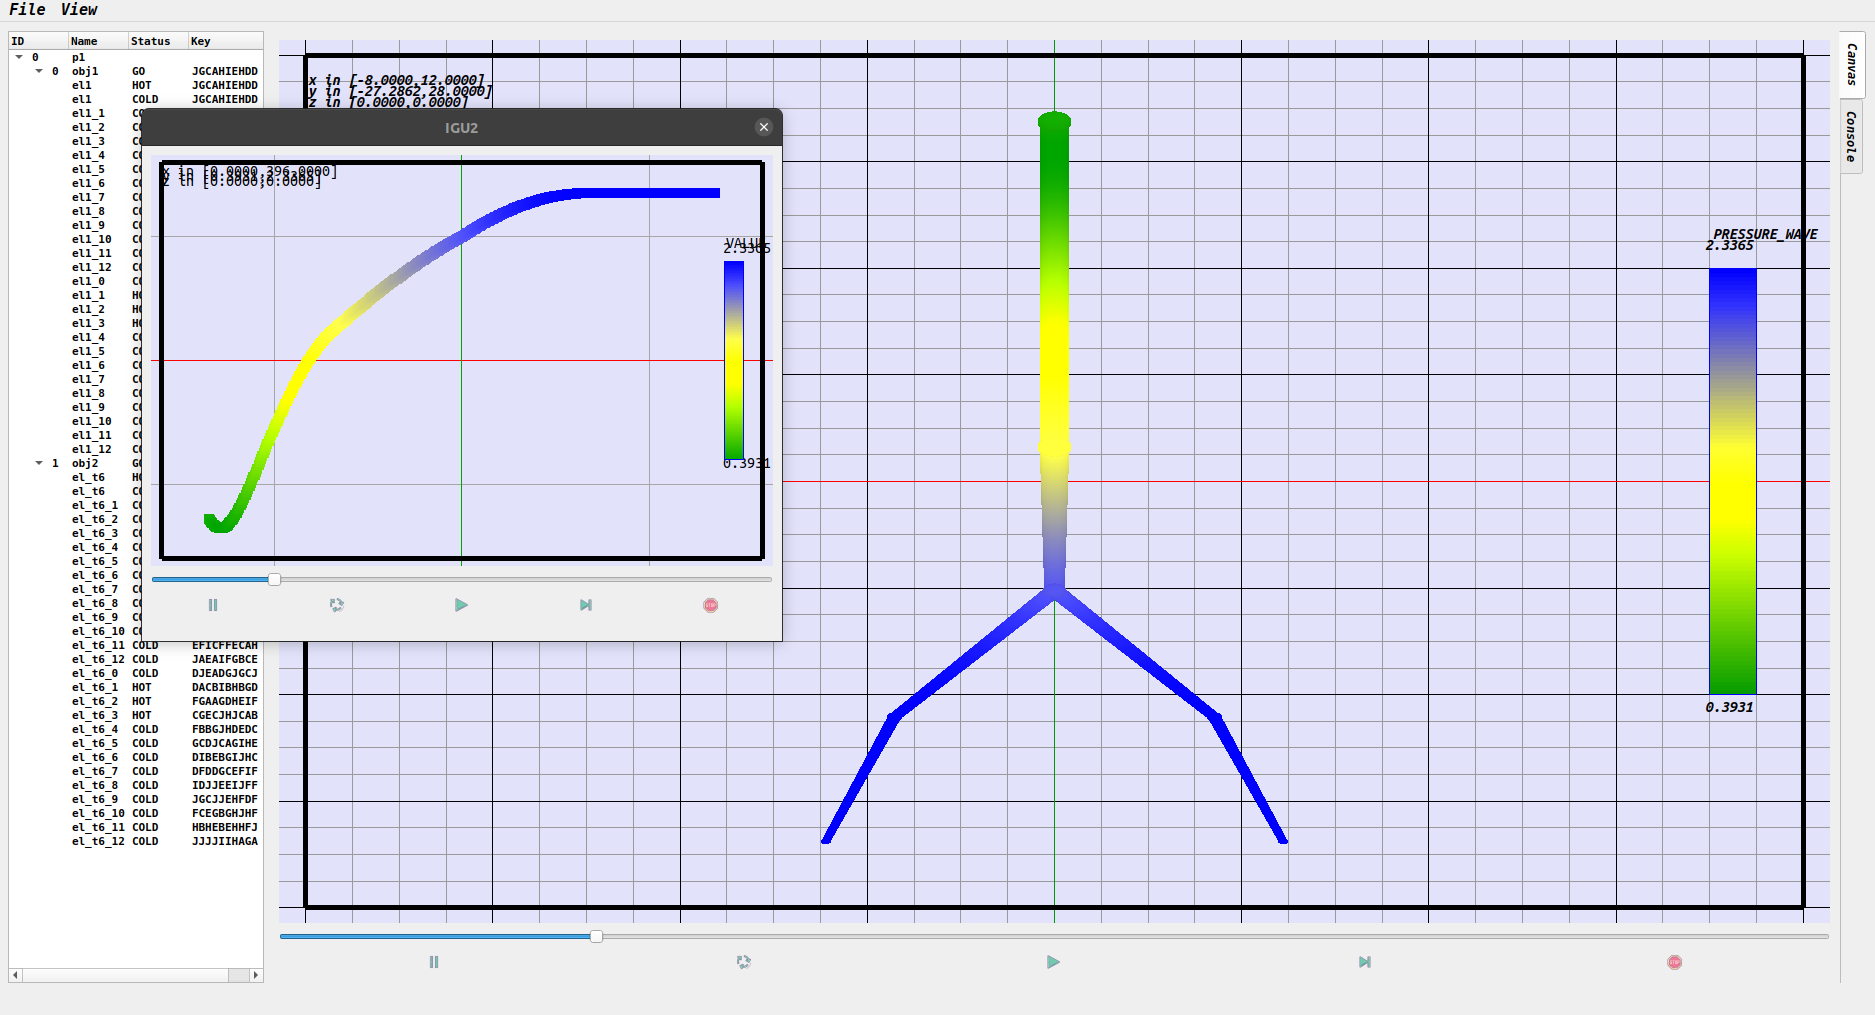
\includegraphics[width=0.7\textwidth]{Figures/IGU_025.png}
		
	\end{center}

	\framebreak
	
	\begin{itemize}
	\item A janela \textit{Jobs} exibe uma listagem compreensiva dos processos inciados e enviados à thread inteligente \textit{WiseThreadPool}, cada comando executado via \textit{Console} ou elemento de interface gráfica irá gerar processos listados nesta janela.
	
	\end{itemize}		
	
	\begin{center}
	
	\item 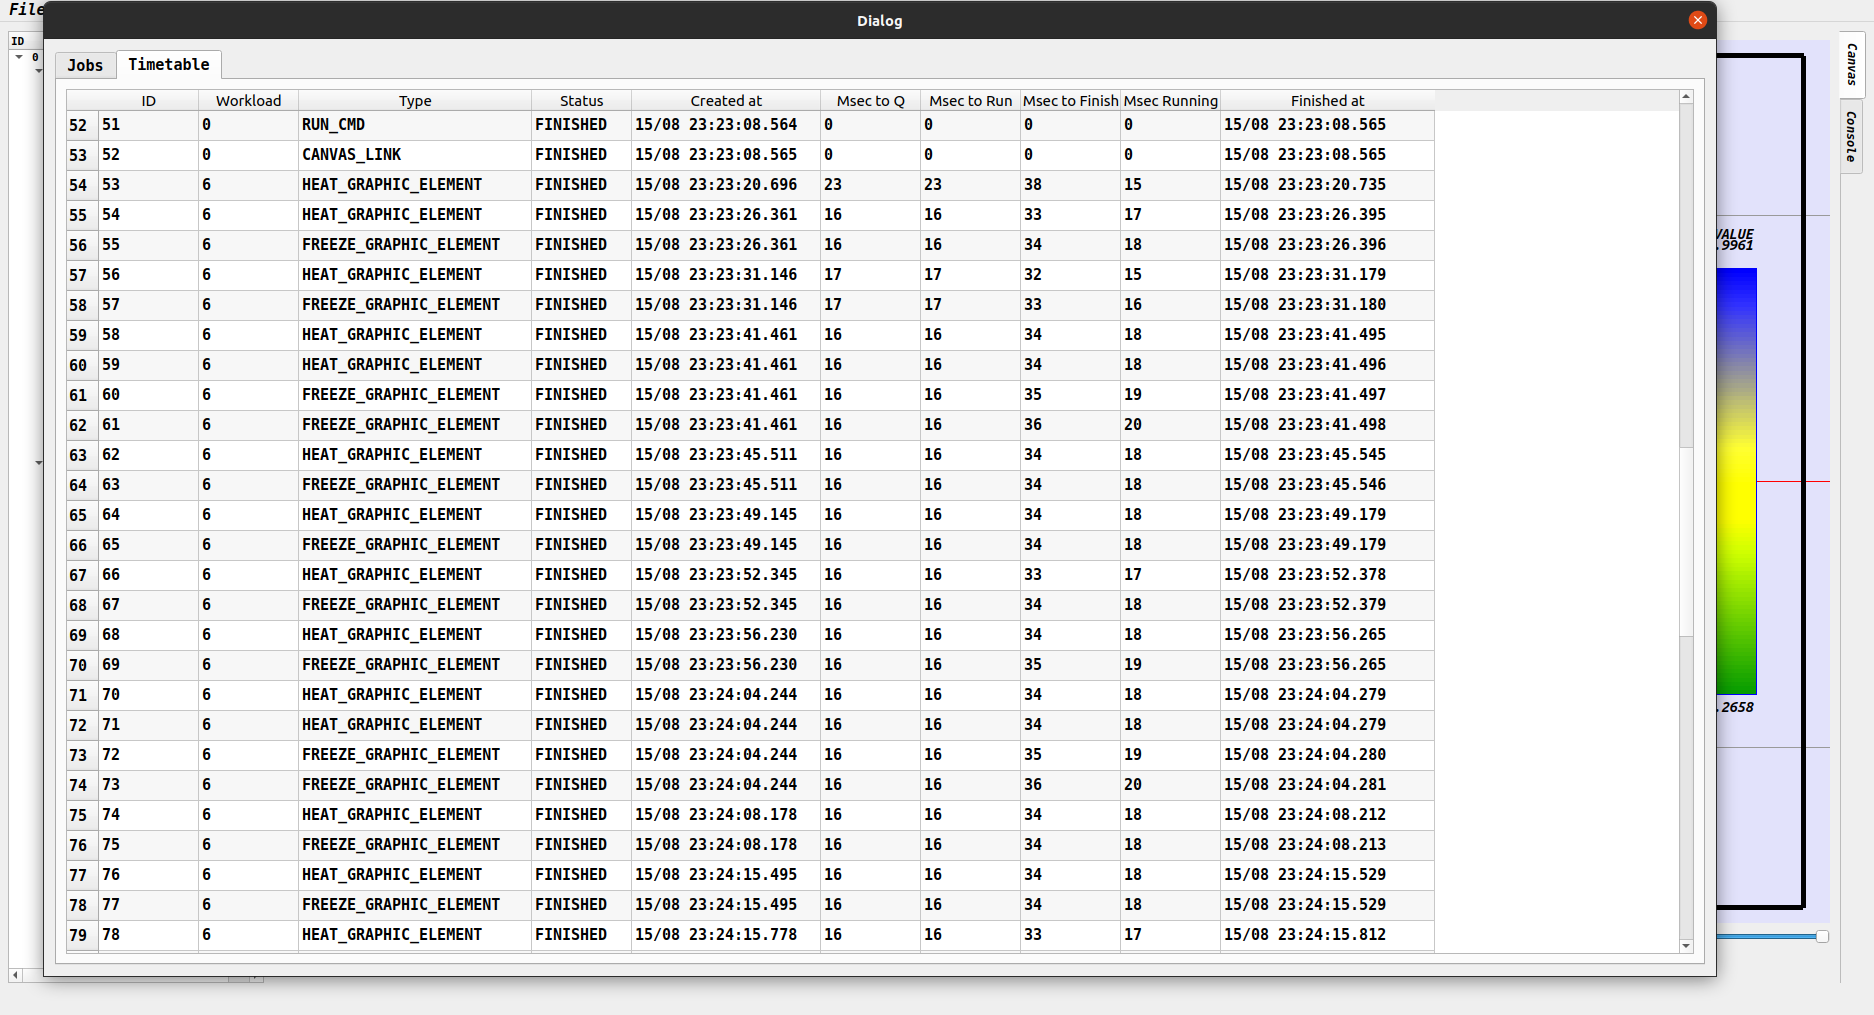
\includegraphics[width=0.6\textwidth]{Figures/IGU_023.png}
	
	\end{center}

	\framebreak
	
	\begin{center}
	\begin{itemize}
		\begin{multicols}{2}
			\vfill
			\item A árvore de projetos apresenta o elemento gráfico da estrutura de projetos carregadas. Na imagem está um projeto nomeado \textit{p1}, um objeto inteligente \textit{obj1} e diversos elementos inteligentes e gráficos. 
			\item Como visto anteriormente quando o objeto está no estado \textit{GO} significa que ele já foi corretamente configurado e iterado. 
			\item Dentro deste objeto inteligente estão os elementos inteligentes e gráficos. 
			\item O primeiro elemento \textit{el1} é o elemento contido na estrutura \textit{Forno} e é o único elemento inteligente no estado \textit{Hot}. 
			\item Em seguida estão os elementos inteligentes da estrutura \textit{Freezer}, seguidos pelos objetos gráficos.
			
			\item Através da árvore de projetos é possível observar a troca de estado dos elementos, por exemplo, ao executar a animação os elementos gráficos serão sucessivamente aquecidos. 
			\item Se observa que a mesma quantidade de elementos gráficos e inteligentes, mantendo a consistência do objeto inteligente, cada passo iterativo com sua respectiva representação gráfica.
			\columnbreak
			\item 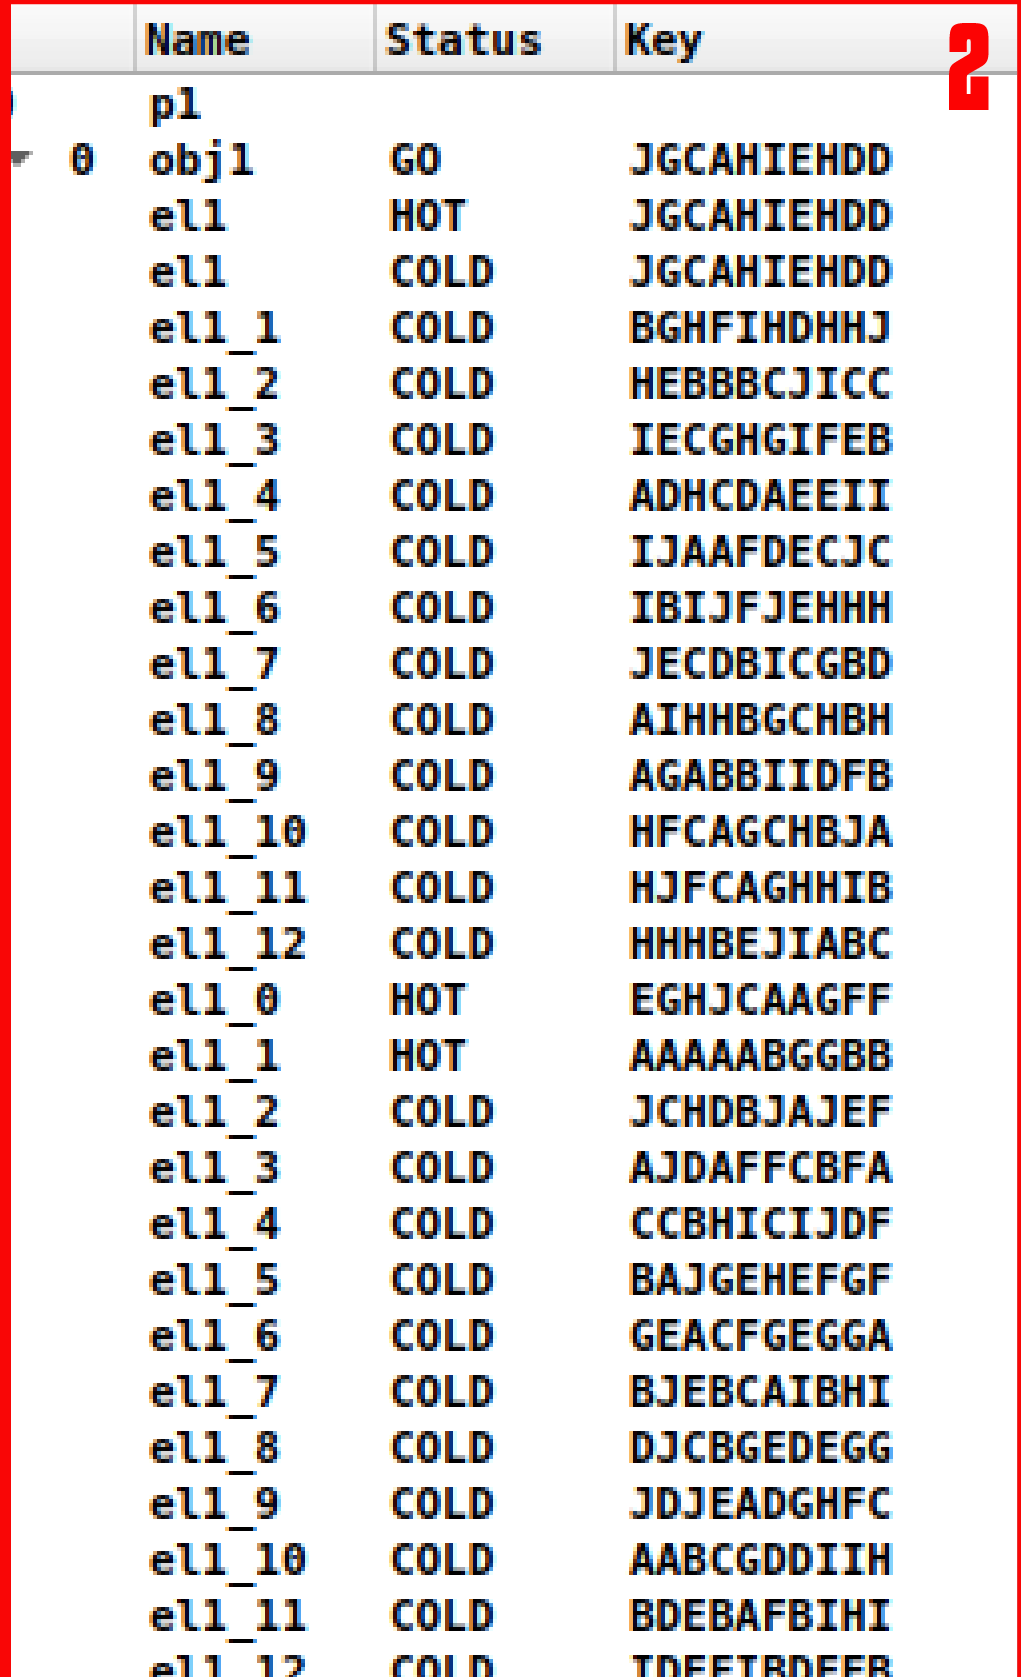
\includegraphics[width=0.35\textwidth]{Figures/IGU_001c.png}
		\end{multicols}
	\end{itemize}
	\end{center}

\end{frame}
	
	
\section{Resultados}
\begin{frame}[allowframebreaks]
	\frametitle{Resultados}
	\begin{center}
		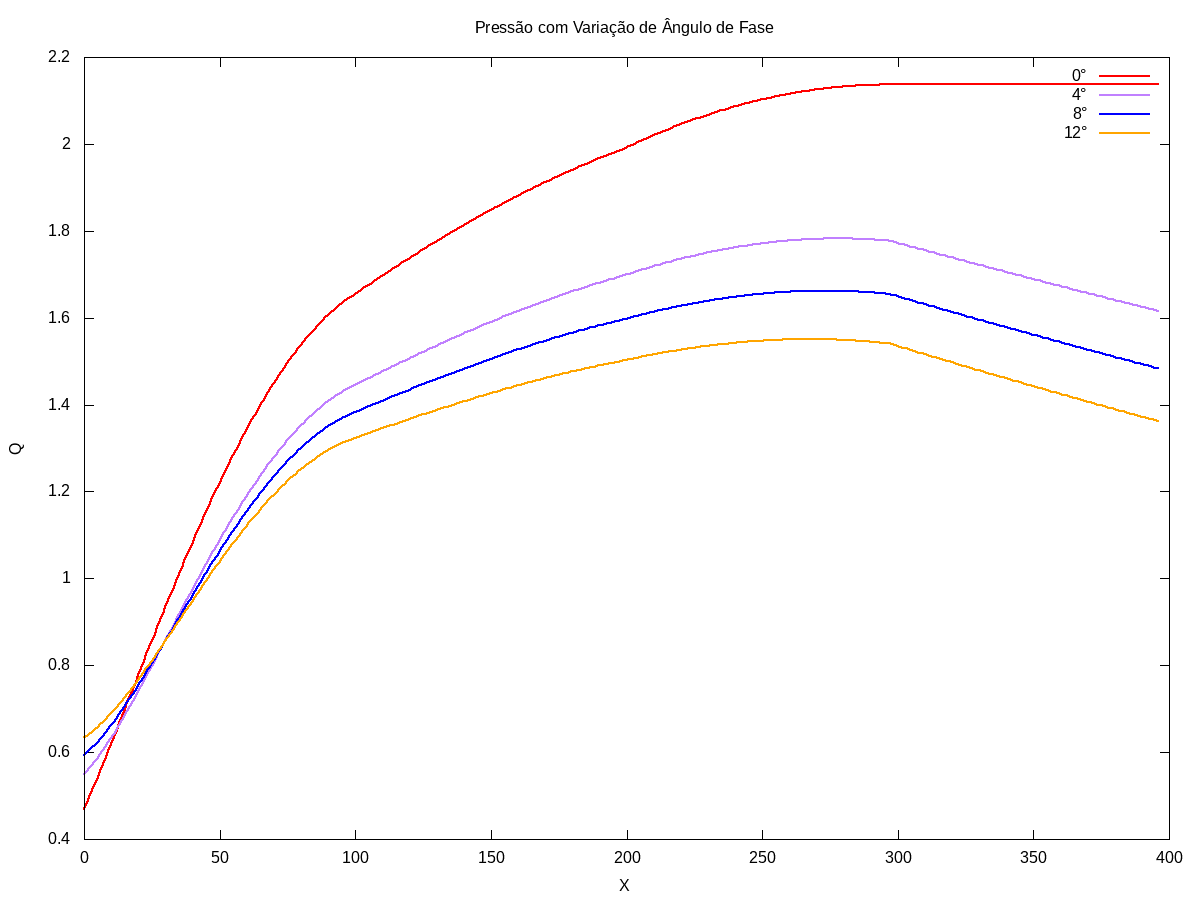
\includegraphics[width=0.4\textwidth]{images/48.png}
		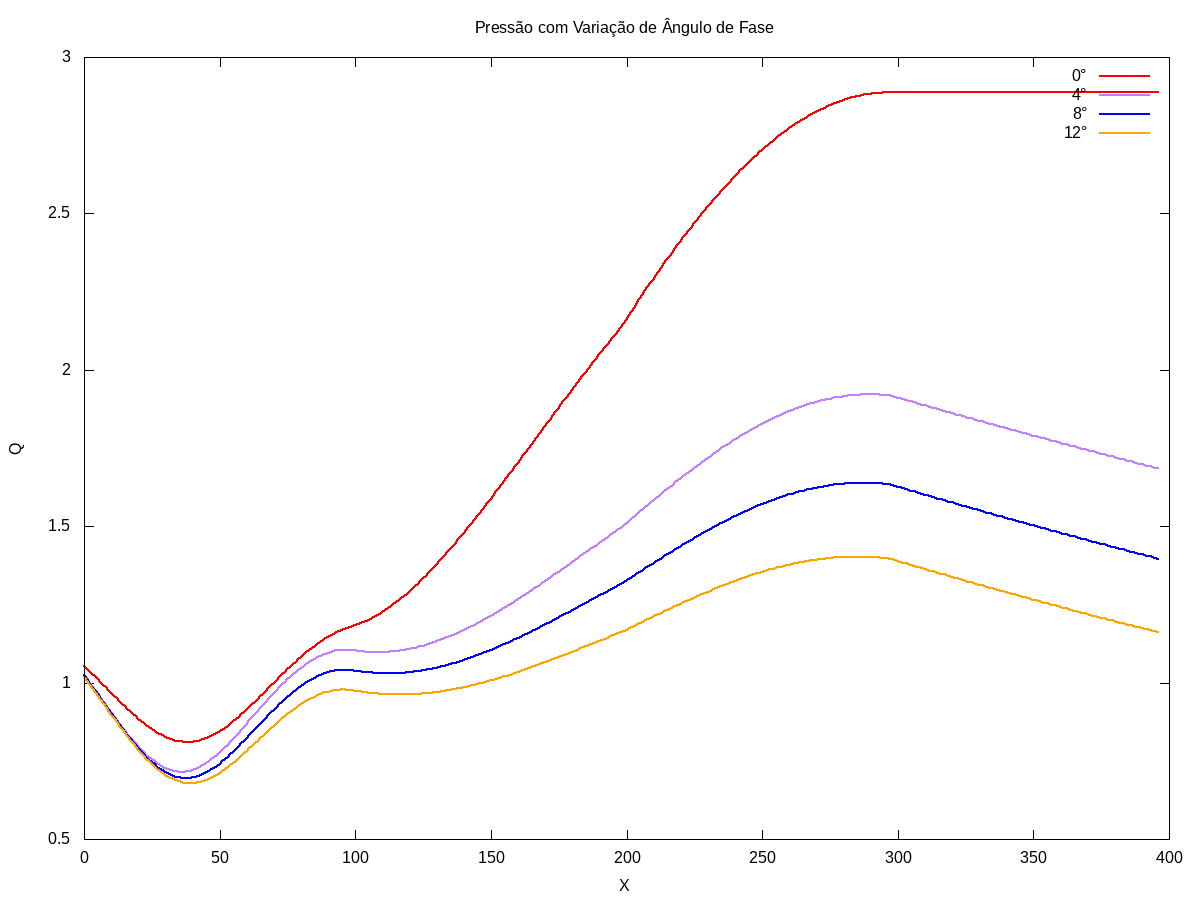
\includegraphics[width=0.4\textwidth]{images/49.png}
		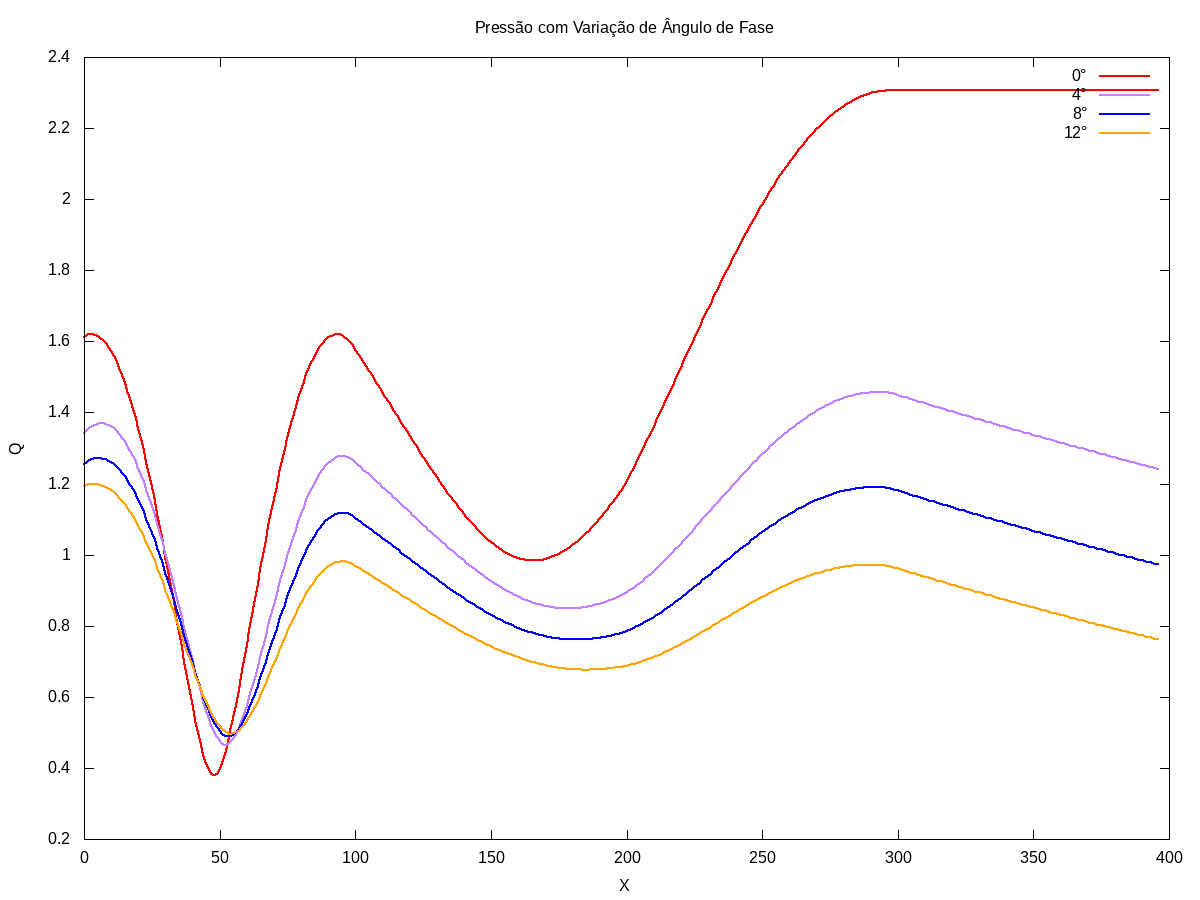
\includegraphics[width=0.4\textwidth]{images/50.png}
		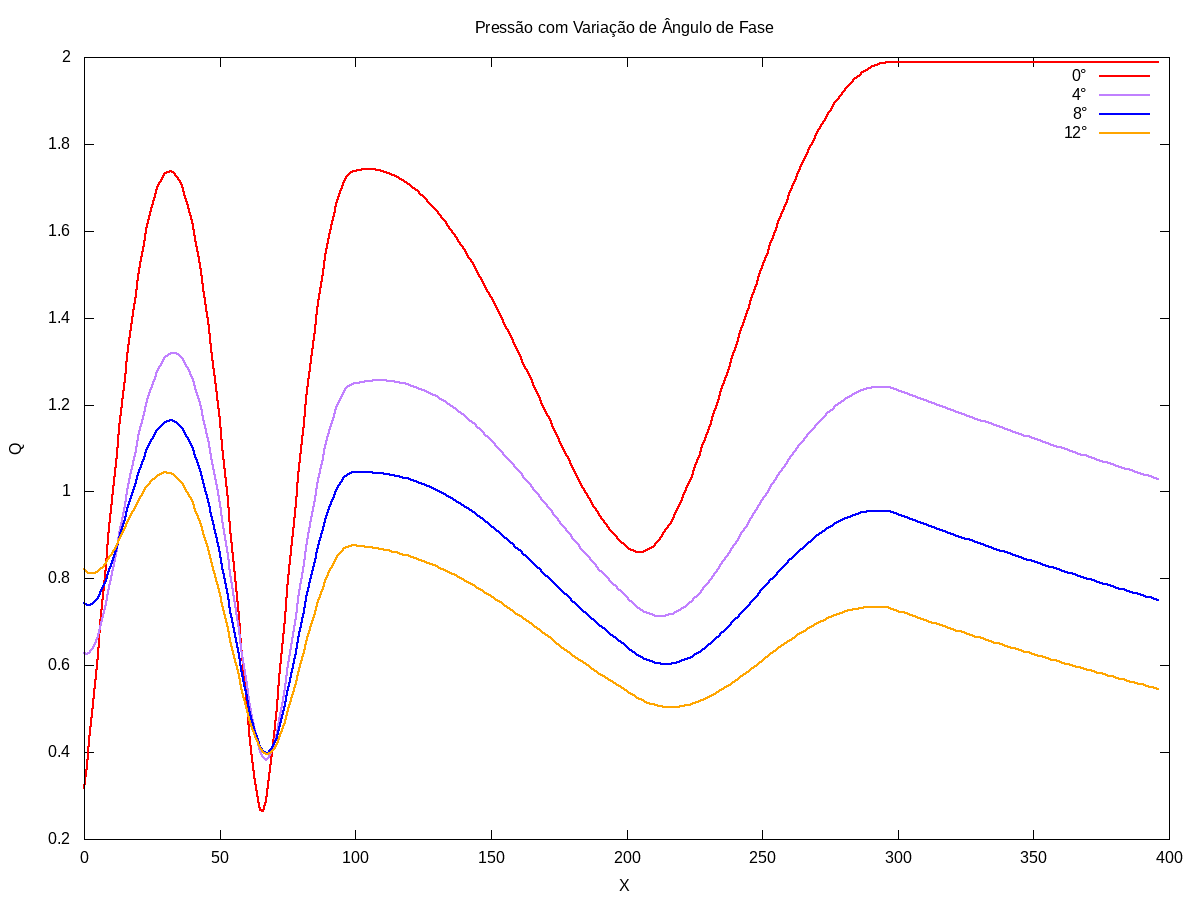
\includegraphics[width=0.4\textwidth]{images/51.png}
	\end{center}
	
	\framebreak
	
	\begin{center}
		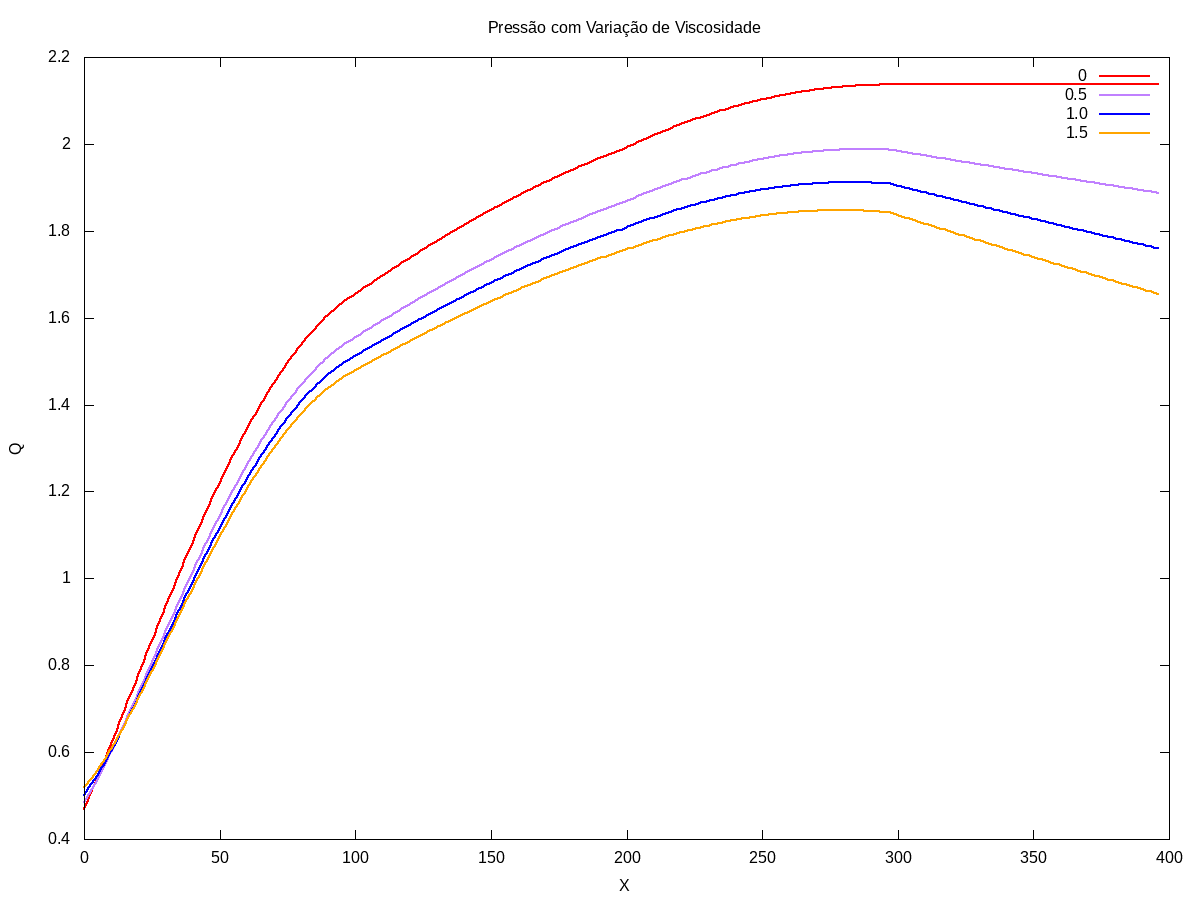
\includegraphics[width=0.4\textwidth]{images/52.png}
		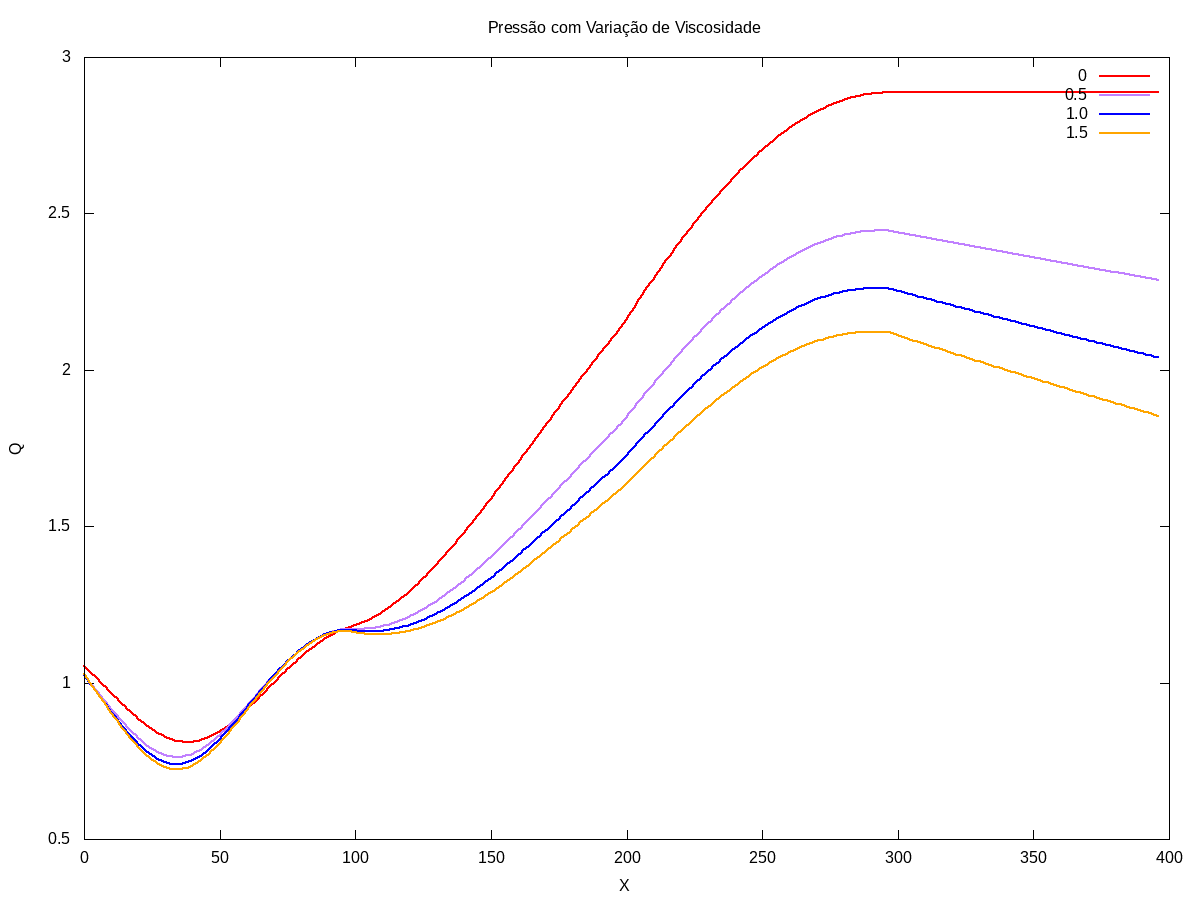
\includegraphics[width=0.4\textwidth]{images/53.png}
		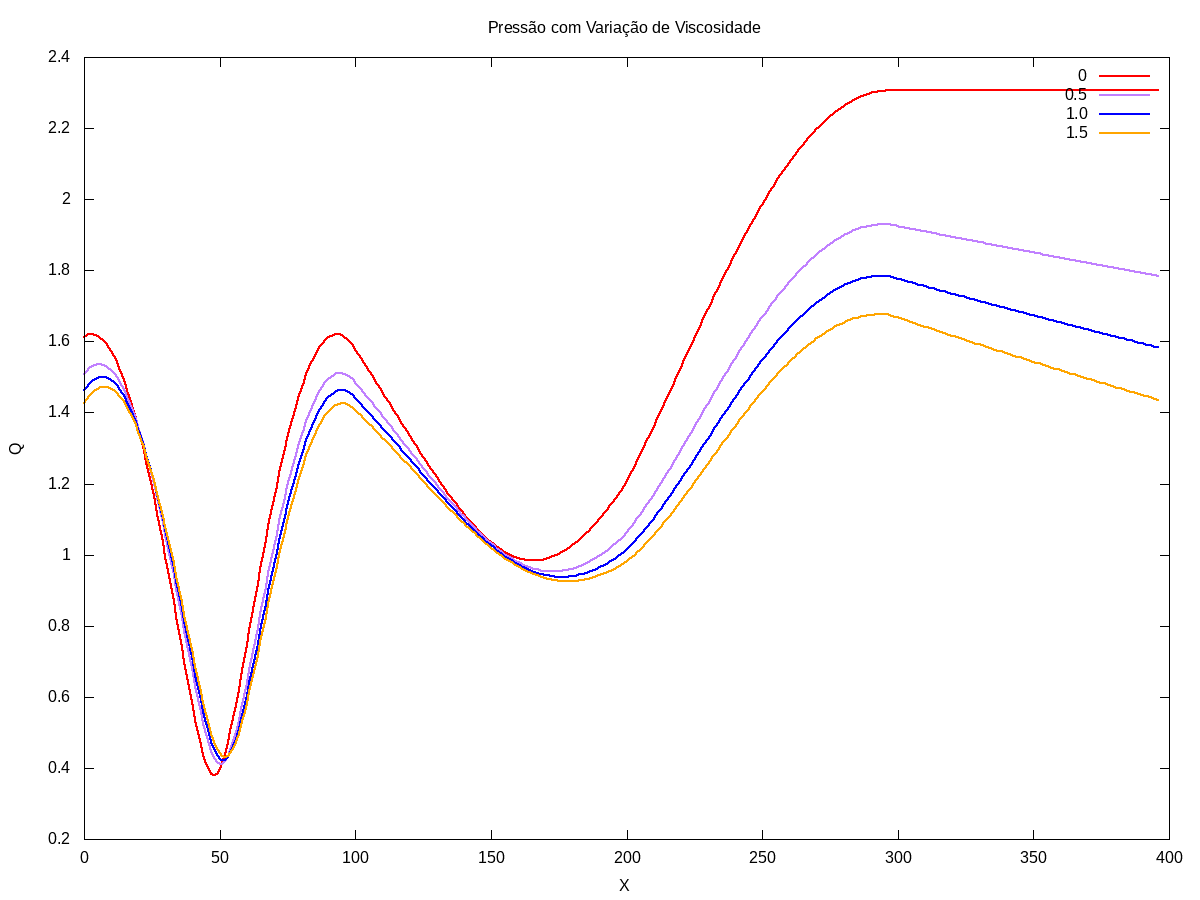
\includegraphics[width=0.4\textwidth]{images/54.png}
		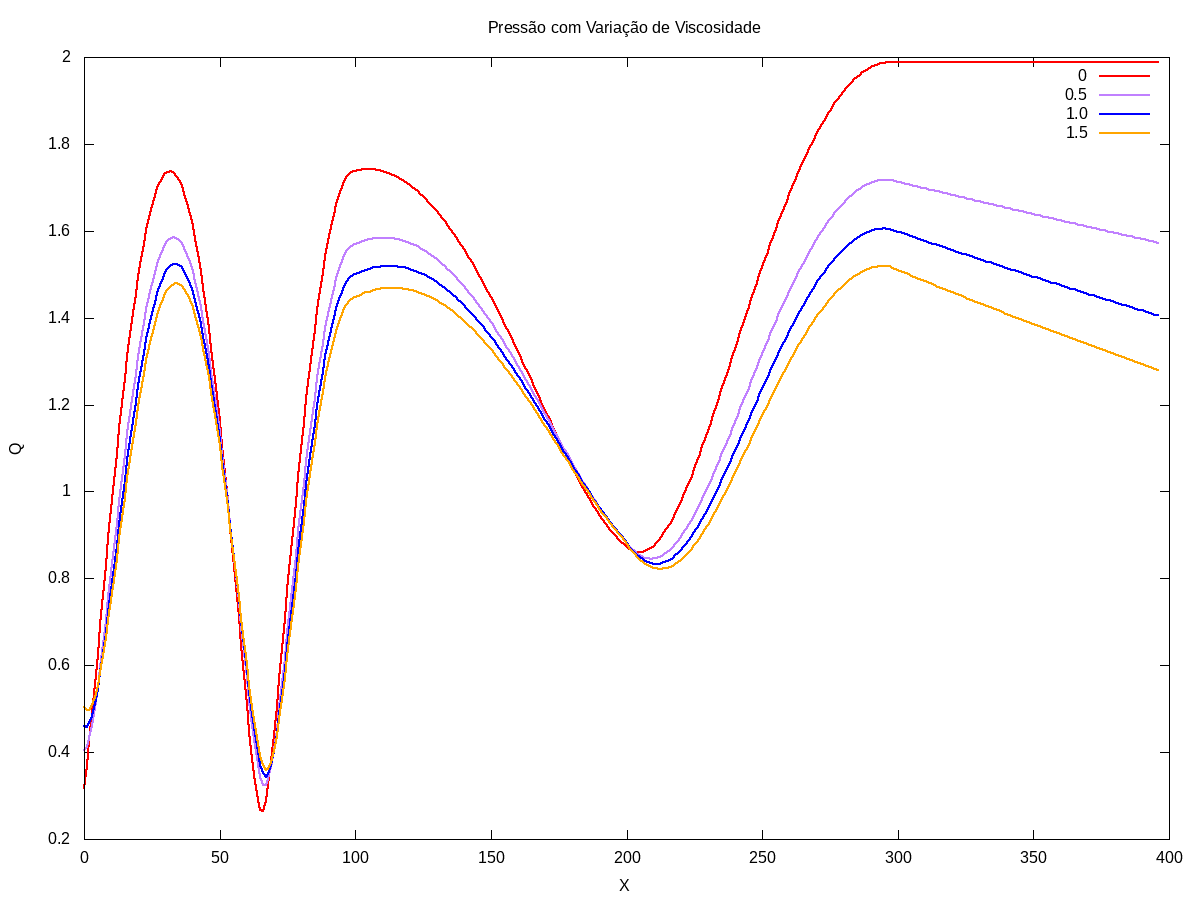
\includegraphics[width=0.4\textwidth]{images/55.png}
	\end{center}

	\framebreak
		
	\begin{center}
		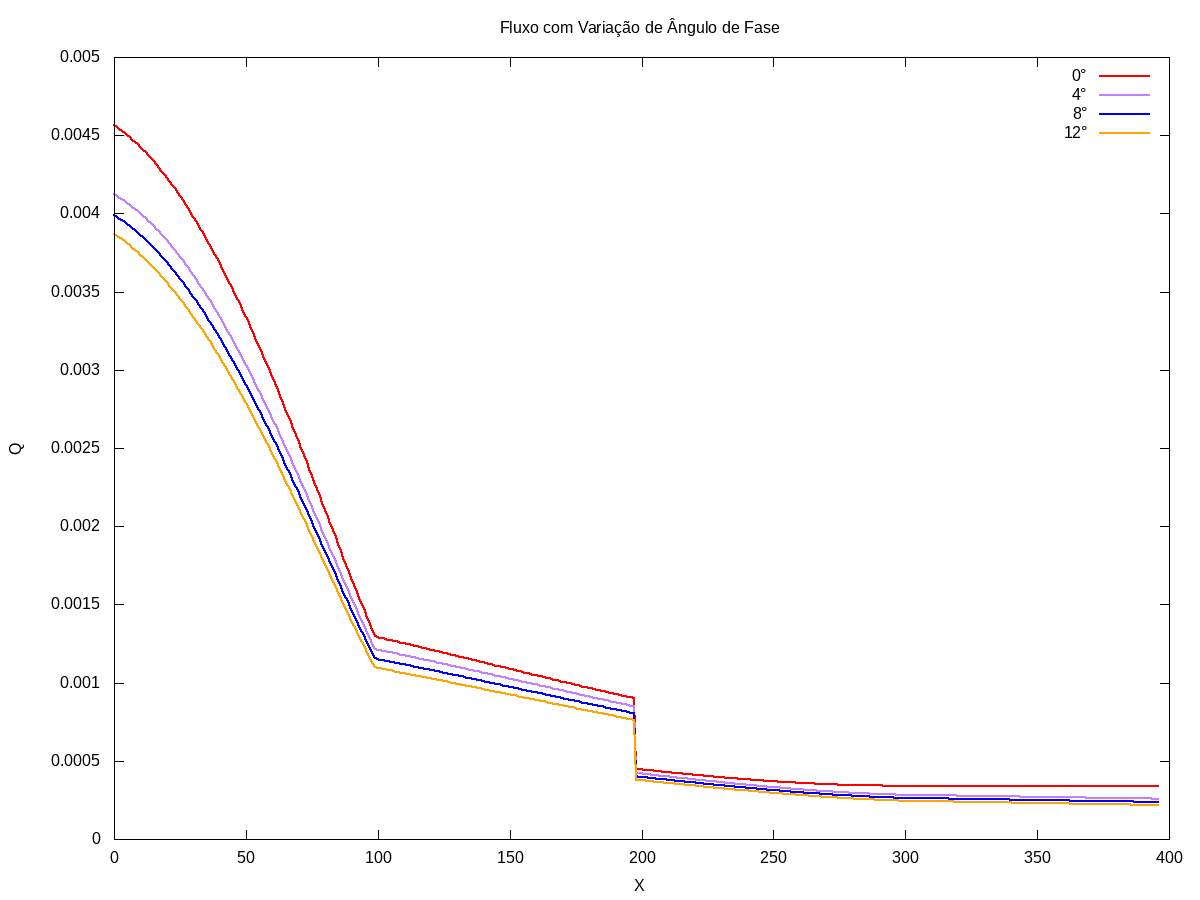
\includegraphics[width=0.4\textwidth]{images/56.png}
		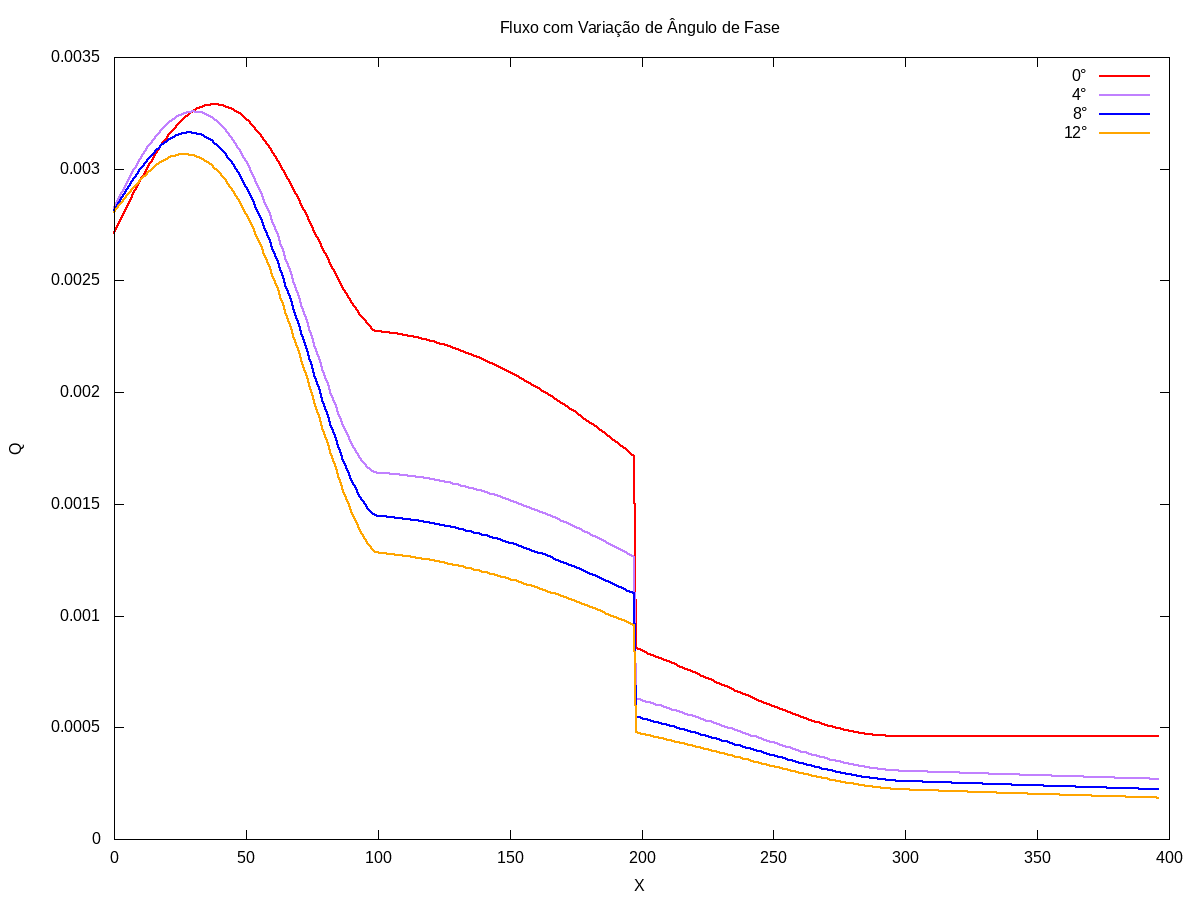
\includegraphics[width=0.4\textwidth]{images/57.png}
		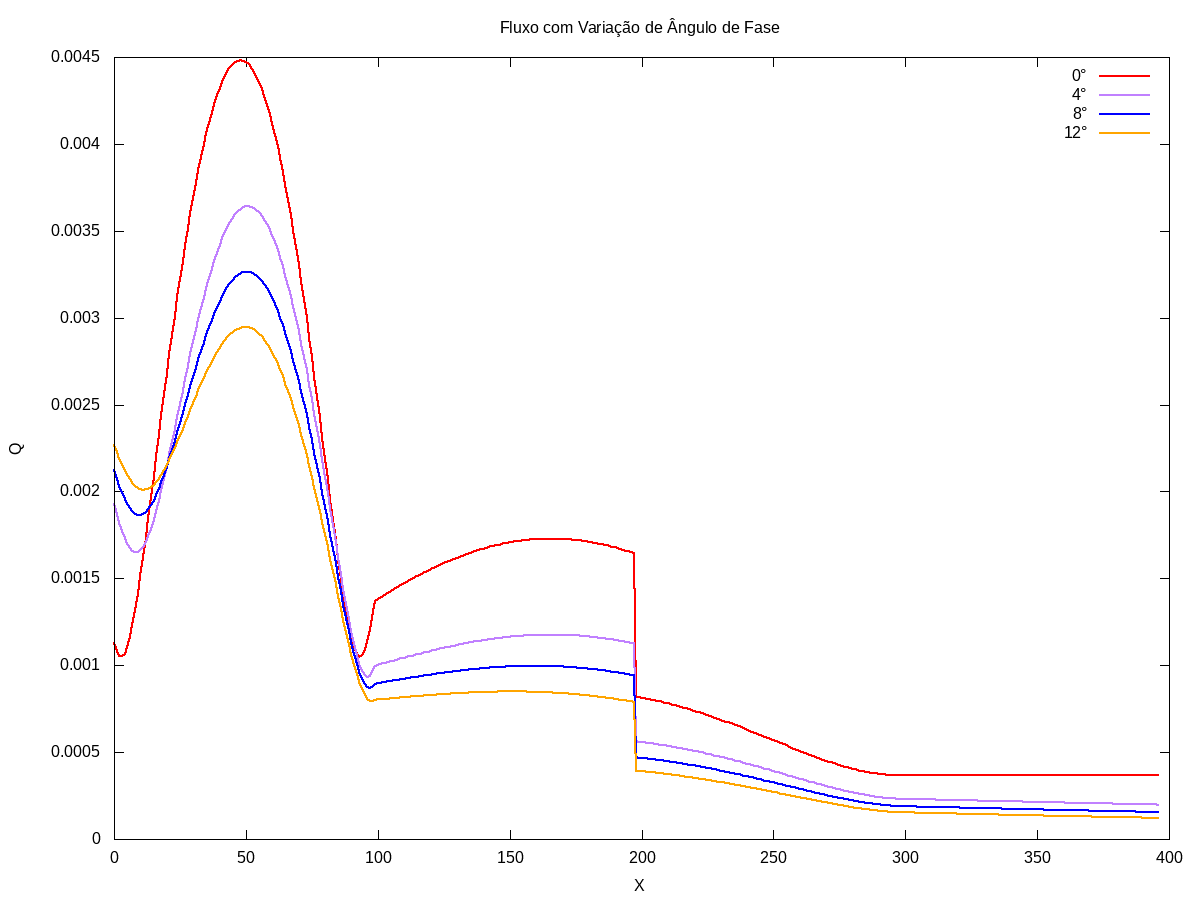
\includegraphics[width=0.4\textwidth]{images/58.png}
		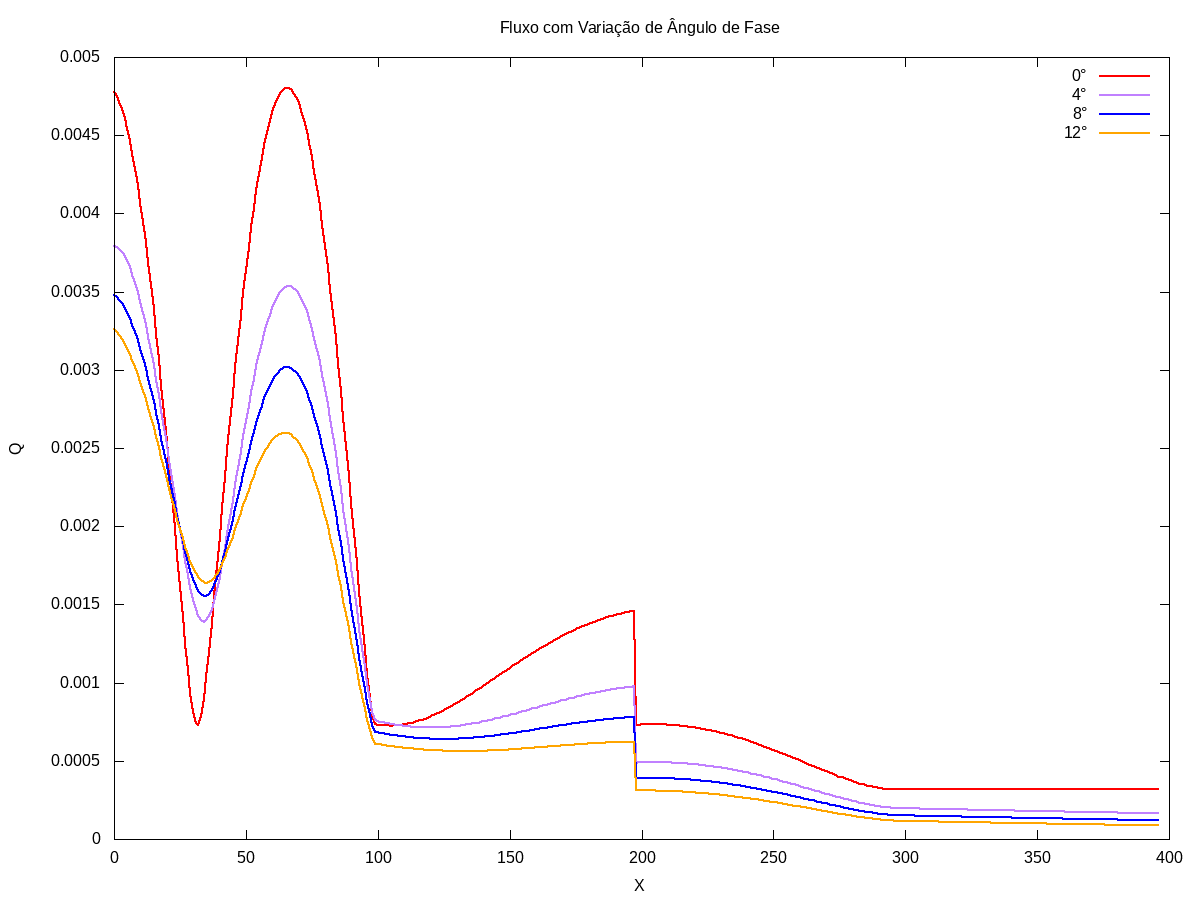
\includegraphics[width=0.4\textwidth]{images/59.png}
	\end{center}
	
	\framebreak
	
	\begin{center}
		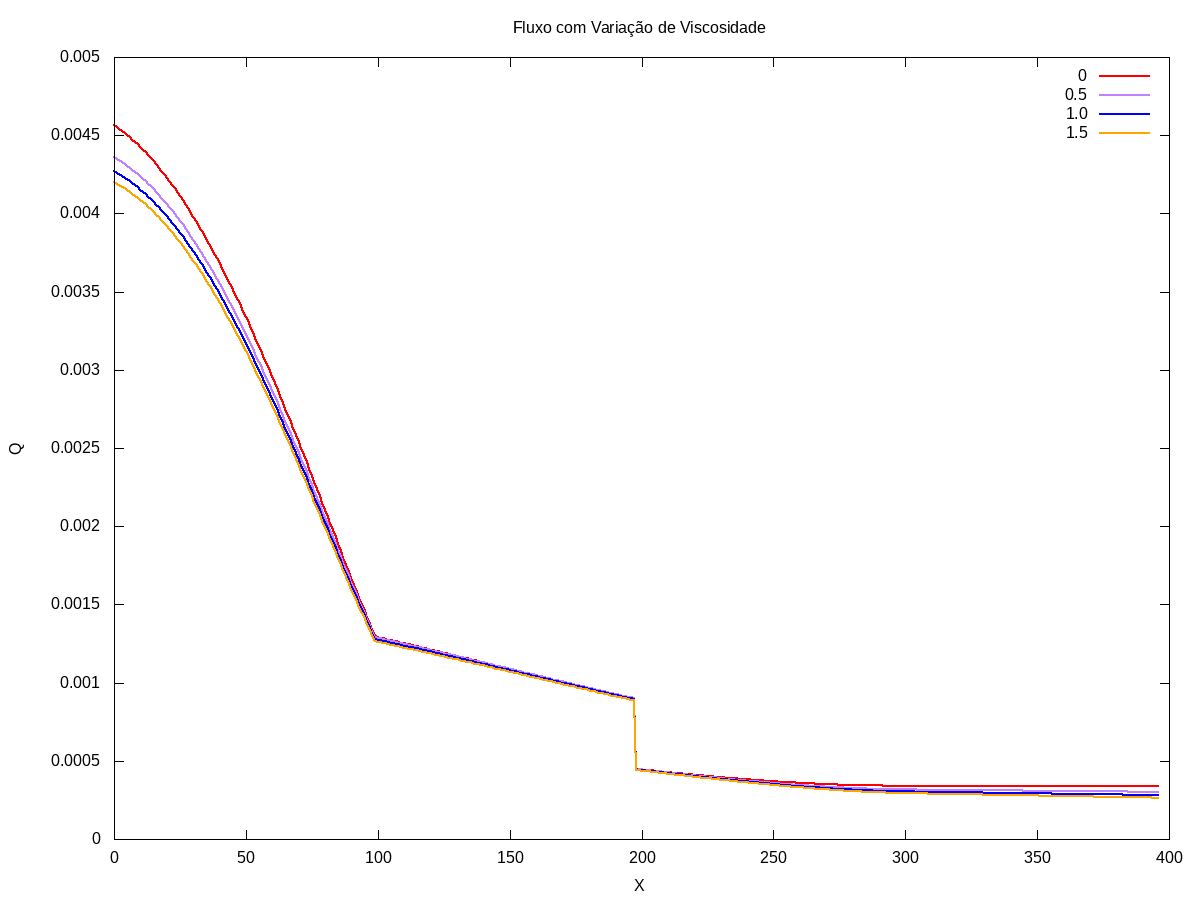
\includegraphics[width=0.4\textwidth]{images/60.png}
		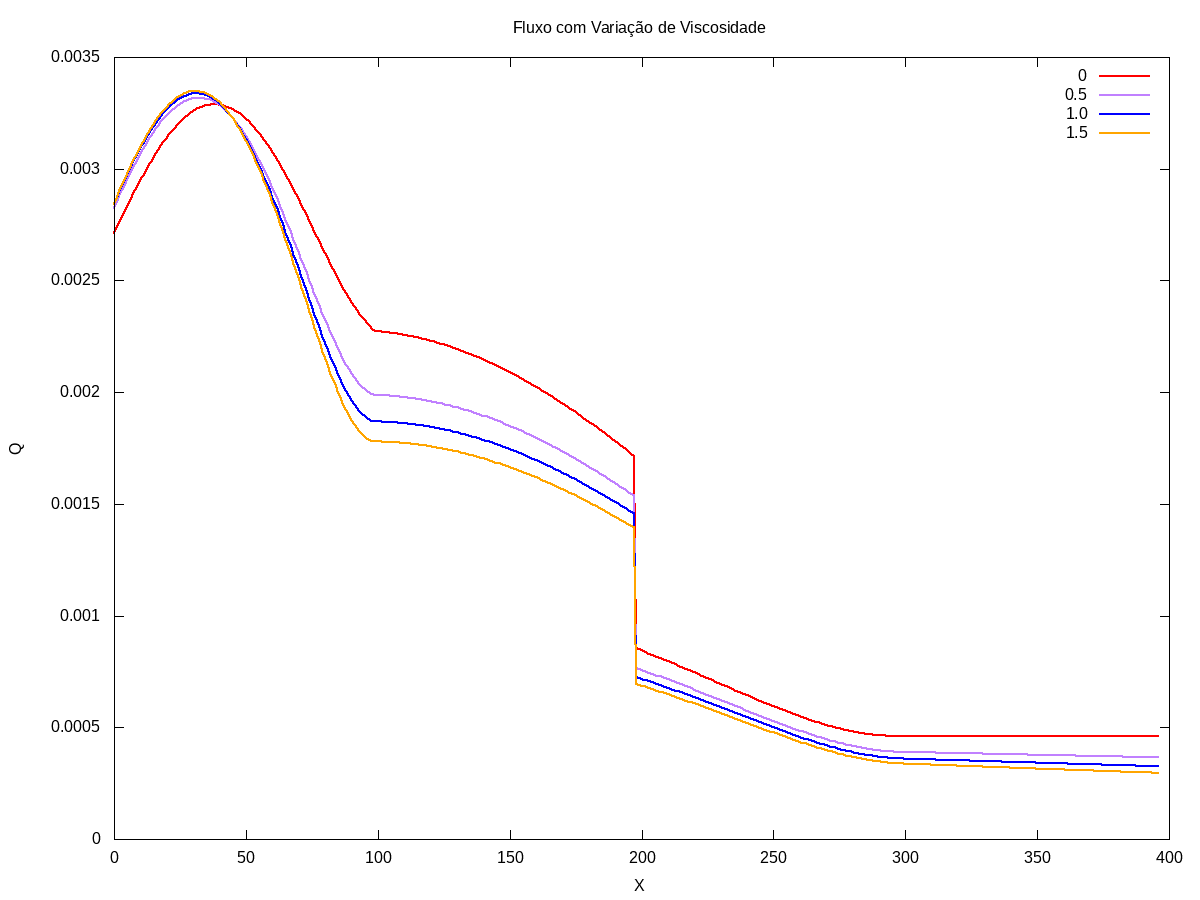
\includegraphics[width=0.4\textwidth]{images/61.png}
		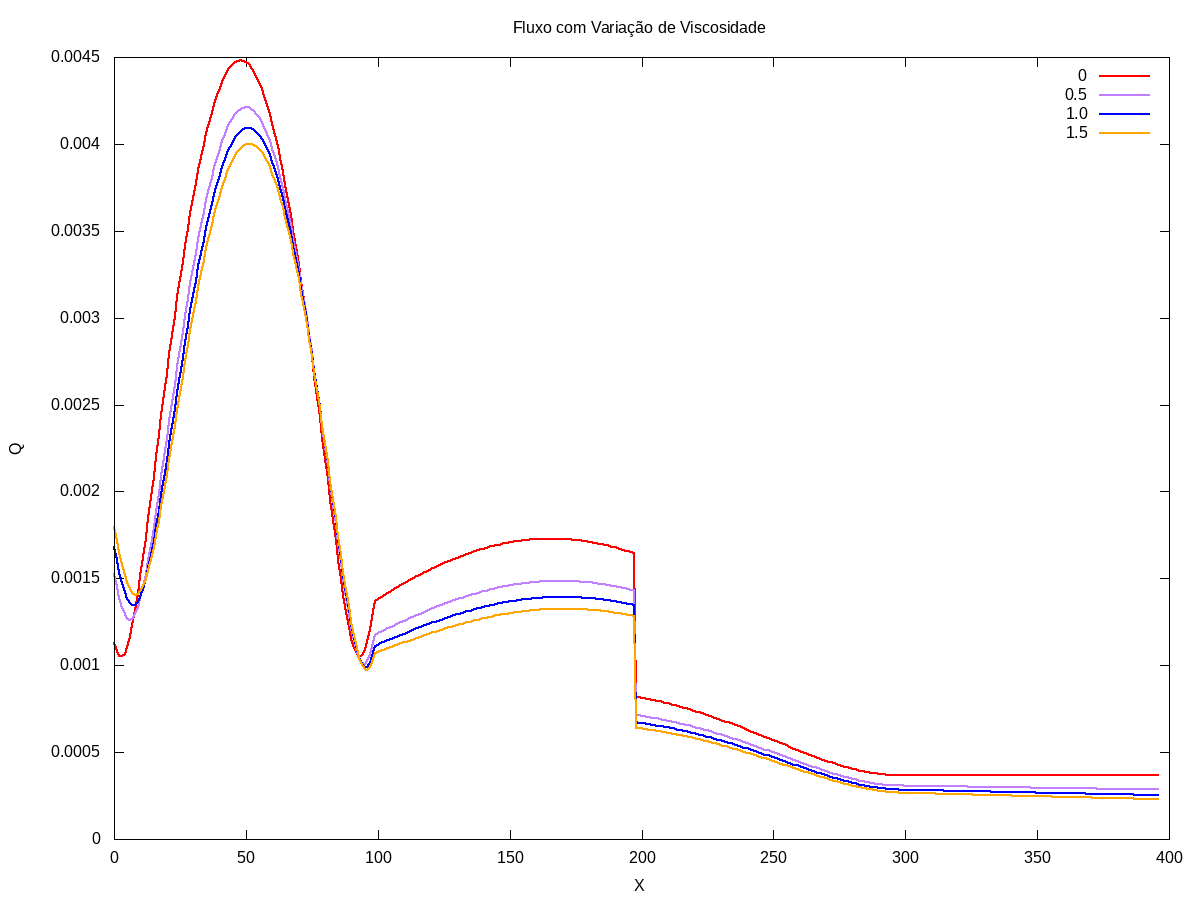
\includegraphics[width=0.4\textwidth]{images/62.png}
		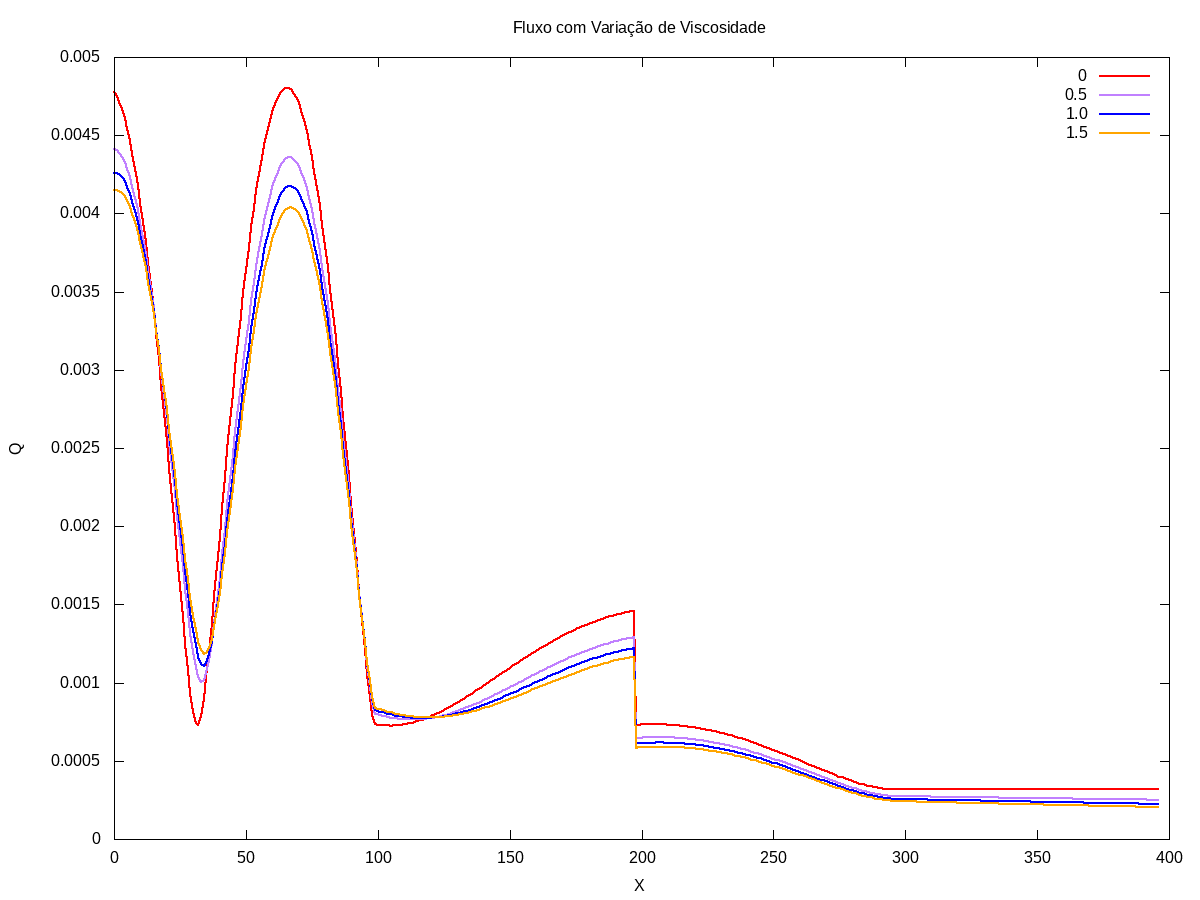
\includegraphics[width=0.4\textwidth]{images/63.png}
	\end{center}

\end{frame}

\section{Dissertação}
\begin{frame}[allowframebreaks]
	\frametitle{Dissertação}
	
	\begin{itemize}
		\item Ferramenta Computacional
		\item Estrutura de dados
		\item \textbf{dividir em elemento inteligente, objeto inteligente e objeto gráfico?}
		\item  (Sinais e slots, paralelização)
		\item Lista de comandos
		\item Interface gráfica
		\item Resultados
		\item Fluxo
		\item Pressão
		\item Conclusão
	\end{itemize}
	
\end{frame}

\section{Cronograma}
\begin{frame}[allowframebreaks]
	\frametitle{Cronograma}
	
	\begin{itemize}
		\item Mar: Ajustes dissertação + Fim da dissertação
		\item Abr: Ajustes finais
		\item Mai: Ajustes finais
	\end{itemize}
	
\end{frame}
	
\end{document}
